
%%% Local Variables:
%%% mode: latex
%%% TeX-master: t
%%% End:
\section{空间数据绘图系统}

\begin{frame}[c]{\subsecname}{}
      \begin{ornamentblock}%\hspace*{\parindent}
\hspace*{2em}我们借助于外感官(我们意识的一种性质)表象给我们自己外面的对象,这些对
象毫无例外的在空间里面。这些对象的形状、大小、以及它们相互间的关系是在
空间里被规定的或能够在空间里被规定的。\\
\hspace*{2em}空间不是一个从外部经验得来的经验概念。因为为使着某种感觉与我以外的某些
东西发生关系,以及同样地为着我能把那些感觉表象为互相在外、互相靠近,从
而不只是彼此不同,并且是在不同的地方,这样就一定要以空间观念为前提。\\
          \rightline{\textemdash《康德·纯粹理性批判》}
      \end{ornamentblock}
\end{frame}

% \subsection{GIS和R}
% \begin{frame}[t]{\subsecname}{}
% \begin{itemize}
% \item GIS的非正式定义\footnotemark[1]:一组强大的工具集,可以用来收集、存储、任意检索、转换和
% 显示\emphText{来自真实世界有特殊用途的空间数据}
% \item R虽然能够分析并提供数据可视化,但是并没有能力从其他数据中区分出空间数据;因此一组R开发者共同
% 实现了R的\emphText{空间数据类包sp}\footnotemark[2],它新增了用于空间数据类和方法的R功能
% \end{itemize}

% \only<2>{
% \begin{block}{\small 空间数据类的优势}
%   \begin{itemize} \footnotesize
%   \item[\PencilLeftDown] 从空间分析包中转换数据更加容易
%   \item[\PencilLeftDown] 提供GIS接口包,可以读写外部GIS格式数据
%   \item[\PencilLeftDown] 实现空间数据组织、绘图、打印的方法
%   \item[\PencilLeftDown] 能够对绘图进行地图修饰(参考网格、指北针、比例尺)
%   \end{itemize}
% \end{block}}

% \footnotetext[1]{
% Burrough, P. A. and McDonnell, R. A. (1998). \emph{Principles of Geographical
% Information Systems}. Oxford University Press, Oxford.}
% \footnotetext[2]{
% Pebesma, E. J. and Bivand, R. S. (2005). \emph{Classes and methods for spatial
% data in R}. R News, 5(2):9–13.}
% \end{frame}

% \subsection{R的空间数据类}
% \begin{frame}[t]{\subsecname}{}
% \begin{itemize}
% \item<1-> sp包从2005年开始提交CRAN,主要创始人是挪威经济学院教授
% \href{https://www.nhh.no/en/employees/faculty/roger-bivand/}{\uline{Roger Bivand}}和
% 慕尼黑大学教授\href{https://www.uni-muenster.de/Geoinformatics/en/institute/staff/index.php/119/Edzer_Pebesma}{\uline{Edzer Pebesma}};目前项目负责人是Edzer,并有稳定的开发团队和成熟的讨论组
% \item<2-> sp包未包含在base包中,需要单独下载使用
% \item<3-> 目前绝大多数空间数据相关的包都会以sp包为基础来编写
% \end{itemize}

% \begin{overlayarea}{\textwidth}{\textheight}
% \only<1>{
% \begin{figure}
% \begin{columns}
%     \begin{column}{.5\textwidth}\centering
%         
\includegraphics[width=0.7\columnwidth]{roger_bivand.jpg}
%     \end{column}

%     \begin{column}{.5\textwidth}\centering
%         
\includegraphics[width=0.55\columnwidth]{edzer_pebesma.jpg}
%     \end{column}
%   \end{columns}
% \caption{sp包的两位主要作者.左边是Roger Bivand,右边是Edzer Pebesma}
% \end{figure}}

% \only<3>{
% \begin{figure}
%     \centering
%     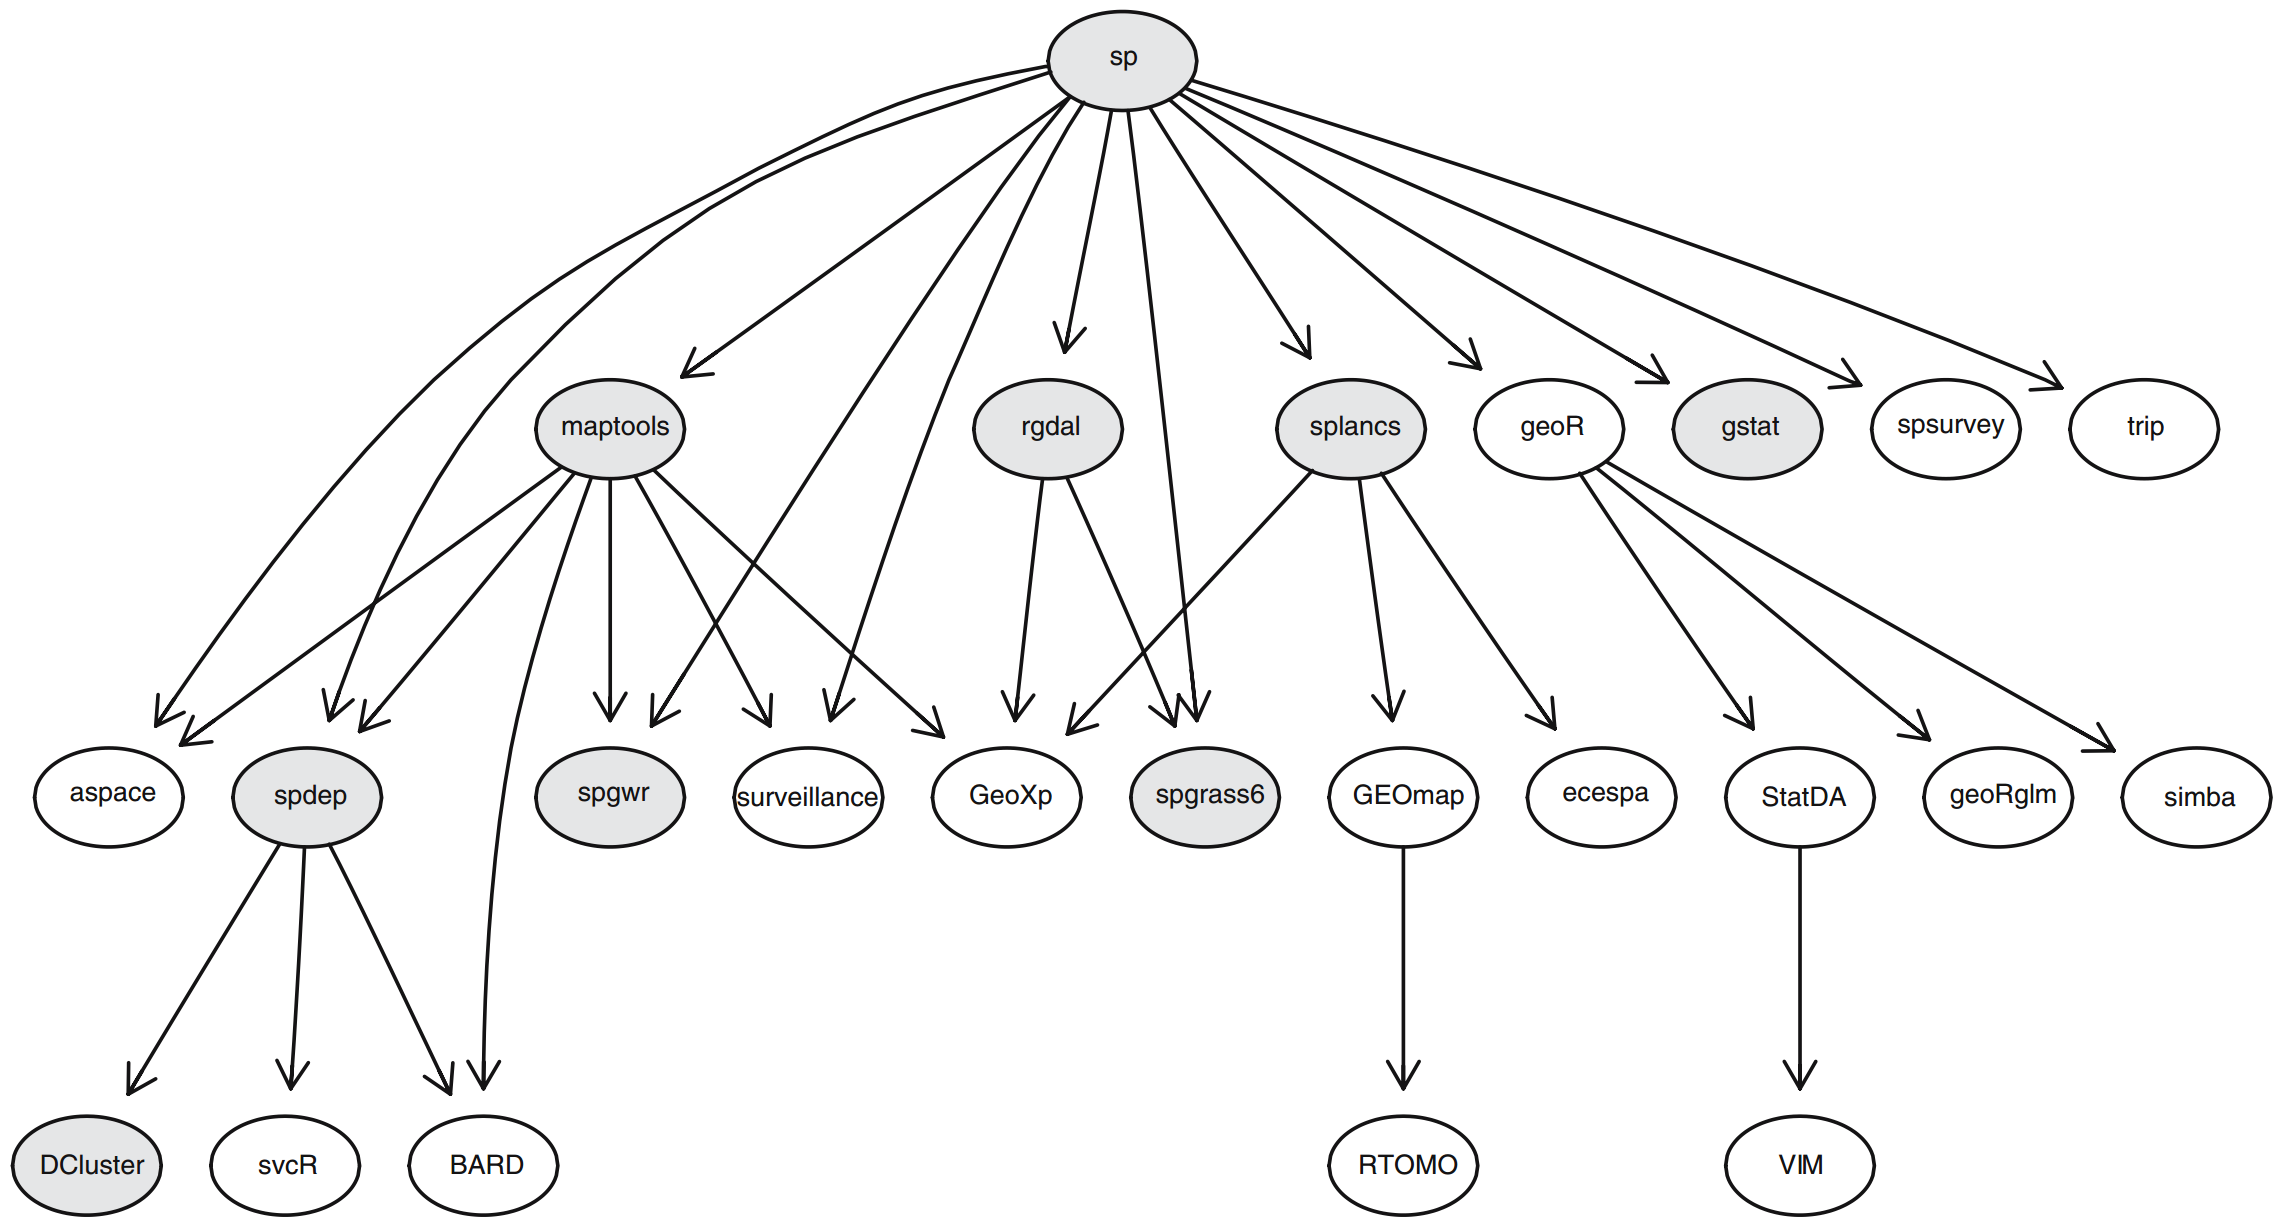
\includegraphics[width=0.8\columnwidth]{sp_depend.png}
%     \caption{直接或间接基于sp包开发的程序包}
% \end{figure}}
% \end{overlayarea}
% \end{frame}

% \begin{frame}[t,fragile]{\subsecname}{}
% \begin{itemize}
% \item<1-> sp包提供的空间类是\emphText{基于S4方法编写的},其\emphText{基类是Spatial}
% \item<2-> Spatial类包括两个属性(slot),一个是matrix类型的\emphText{约束盒}(bbox),
% 另一个是CRS类型的\emphText{坐标参考系统}(proj4string)
% \item<3-> 约束盒是列名为\emphText{c('min','max')}的坐标矩阵,至少有两列,一列指向东(x轴),一列
% 指向北(y轴);CRS类只有一个属性,其值是一个\emphText{\href{http://proj4.org/}{\uline{PROJ.4}}开源CRS格式的字符串}
% \end{itemize}

% \begin{overlayarea}{\textwidth}{\textheight}
% \begin{onlyenv}<2>
% \begin{rcode}
% > library(sp)
% > getClass("Spatial")
% Class "Spatial" [package "sp"]

% Slots:
                              
% Name:         |\colorbox{green}{bbox}| |\colorbox{green}{proj4string}|
% Class:      matrix         CRS

% Known Subclasses: 
% Class "SpatialPoints", directly
% Class "SpatialMultiPoints", directly
% Class "SpatialGrid", directly
% Class "SpatialLines", directly
% Class "SpatialPolygons", directly
% Class "SpatialPointsDataFrame", by class "SpatialPoints", distance 2
% Class "SpatialPixels", by class "SpatialPoints", distance 2
% Class "SpatialMultiPointsDataFrame", by class "SpatialMultiPoints", distance 2
% Class "SpatialGridDataFrame", by class "SpatialGrid", distance 2
% Class "SpatialLinesDataFrame", by class "SpatialLines", distance 2
% Class "SpatialPixelsDataFrame", by class "SpatialPoints", distance 3
% Class "SpatialPolygonsDataFrame", by class "SpatialPolygons", distance 2
% \end{rcode}
% \end{onlyenv}

% \begin{onlyenv}<3>
% \begin{rcode}
% # 定义约束盒
% > bb <- matrix(c(114.25, 22.45, 114.85, 23.16), ncol = 2, dimnames = list(NULL, c("min", "max")))
% # 新建一个Spatial对象,CRS对象是经纬度坐标系统
% > Spatial(bb, proj4string = CRS("+proj=longlat"))
% An object of class "Spatial"
% Slot "bbox":
%         min    max
% [1,] 114.25 114.85
% [2,]  22.45  23.16

% Slot "proj4string":
% CRS arguments: +proj=longlat
% \end{rcode}
% \end{onlyenv}
% \end{overlayarea}
% \end{frame}

% \subsubsection{空间点类}
% \begin{frame}[t,fragile]{\subsecname}{\subsubsecname}
% \begin{itemize}
% \item<1-> 空间点在GIS中是一个坐标向量,sp包中定义\emphText{SpatialPoints}类来表达空间点
% \item<2-> 相比Spatial类,SpatialPoints类扩展了一个matrix类型的属性\emphText{coords}来存储点坐标矩阵
% \end{itemize}

% \begin{overlayarea}{\textwidth}{\textheight}
% \begin{onlyenv}<2->
% \begin{rcode}
% > getClass("SpatialPoints")
% Class "SpatialPoints" [package "sp"]

% Slots:
                                          
% Name:       |\colorbox{green}{coords}|        bbox proj4string
% Class:      matrix      matrix         CRS

% Extends: "Spatial"

% Known Subclasses: 
% Class "SpatialPointsDataFrame", directly
% Class "SpatialPixels", directly
% Class "SpatialPixelsDataFrame", by class "SpatialPixels", distance 2
% \end{rcode}
% \end{onlyenv}

% \begin{onlyenv}<3>
% \begin{rcode}
% # 读取格式化文件到一个data.frame类型对象CRAN\_df,包含位置经纬度坐标
% > CRAN_df <- read.table("data/CRAN051001a.txt", header = TRUE)
% # 将经纬度坐标构建一个新的matrix类型对象CRAN\_mat
% > CRAN_mat <- cbind(CRAN_df$long, CRAN_df$lat)

% # 构建一个CRS对象llCRS 
% llCRS <- CRS("+proj=longlat +ellps=WGS84")
% # 构建SpatialPoints对象
% CRAN_sp <- |\colorbox{green}{SpatialPoints}|(CRAN_mat, proj4string = llCRS)
% \end{rcode}
% \end{onlyenv}
% \end{overlayarea}
% \end{frame}

% \begin{frame}[t,fragile]{\subsecname}{\subsubsecname}
% \begin{itemize}
% \item<1-> \emphText{SpatialPointsDataFrame}类将SpatialPoints对象转换为类似data.frame数据结构
% \item<2-> SpatialPointsDataFrame类通过coords行名和data.frame行名的对应顺序来构建,
% \emphText{可以用于在空间信息后面挂载属性信息}
% \item<4-> SpatialPointsDataFrame对象有两个索引,一个用于空间对象,另一个用于列
% \end{itemize}

% \begin{overlayarea}{\textwidth}{\textheight}
% \begin{onlyenv}<1>
% \begin{rcode}
% > getClass("SpatialPointsDataFrame")
% Class "SpatialPointsDataFrame" [package "sp"]

% Slots:                                                                  

% Name:         data  coords.nrs      coords        bbox proj4string
% Class:  data.frame     numeric      matrix      matrix         CRS

% Extends: 
% Class "SpatialPoints", directly
% Class "Spatial", by class "SpatialPoints", distance 2
% \end{rcode}
% \begin{figure}[ht]\vspace{-10pt}
%   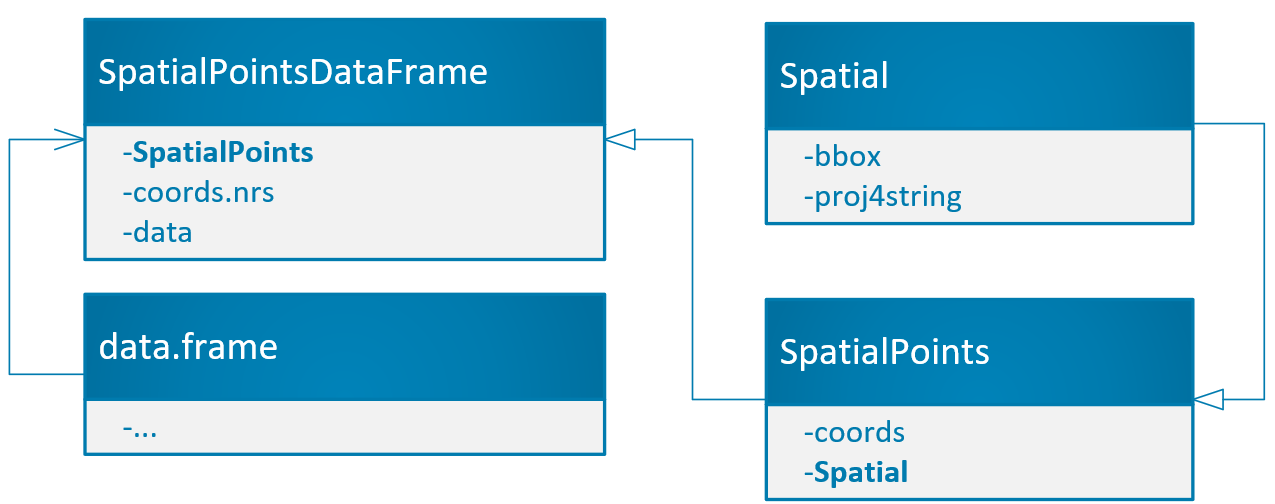
\includegraphics[width=0.6\columnwidth]{spatialpointsdataframe_class.png}
% \end{figure}
% \end{onlyenv}

% \begin{onlyenv}<2>
% \begin{rcode}
% # 将matrix的序号作为行名
% > row.names(CRAN_mat) <- 1:nrow(CRAN_mat)
% > str(CRAN_mat)
%  num [1:54, 1:2] 153 145 16.3 -49.3 -42.9 ...
%  - attr(*, "dimnames")=List of 2
%   ..$ : chr [1:54] "1" "2" "3" "4" ...
%   ..$ : NULL

% # 构建Spatialpoints对象CRAN\_spdf1,match.ID=TURE表示根据CRAN\_mat行名和CRAN\_df行名要对应
% > CRAN_spdf1 <- |\colorbox{green}{SpatialPointsDataFrame}|(coords=CRAN_mat, data=CRAN_df, proj4string=llCRS, match.ID=TRUE)
% \end{rcode}
% \end{onlyenv}

% \begin{onlyenv}<3>
% \begin{rcode}
% # 构建的新对象在空间信息基础上挂载了属性信息long、lat、place、north、east和loc
% > str(CRAN_spdf1)
% Formal class 'SpatialPointsDataFrame' [package "sp"] with 5 slots
%   ..@ data       :'data.frame': 54 obs. of  6 variables:
%   .. ..$ place: Factor w/ 52 levels "Aalborg","Aizu",..: 9 30 50 15 49 39 36 40 12 46 ...
%   .. ..$ north: Factor w/ 52 levels "20d45'S","22d43'S",..: 8 18 41 7 1 3 2 4 43 29 ...
%   .. ..$ east : Factor w/ 51 levels "0d10'W","118d15'W",..: 19 16 20 35 31 32 34 33 11 39 ...
%   .. ..$ loc  : Factor w/ 30 levels "Australia","Austria",..: 1 1 2 3 3 3 3 3 4 19 ...
%   .. ..$ long : num [1:54] 153 145 16.3 -49.3 -42.9 ...
%   .. ..$ lat  : num [1:54] -27.5 -37.8 48.2 -25.4 -20.8 ...
%   ..@ coords.nrs : num(0) 
%   ..@ coords     : num [1:54, 1:2] 153 145 16.3 -49.3 -42.9 ...
%   .. ..- attr(*, "dimnames")=List of 2
%   .. .. ..$ : chr [1:54] "1" "2" "3" "4" ...
%   .. .. ..$ : chr [1:2] "coords.x1" "coords.x2"
%   ..@ bbox       : num [1:2, 1:2] -123 -37.8 153 57
%   .. ..- attr(*, "dimnames")=List of 2
%   .. .. ..$ : chr [1:2] "coords.x1" "coords.x2"
%   .. .. ..$ : chr [1:2] "min" "max"
%   ..@ proj4string:Formal class 'CRS' [package "sp"] with 1 slot
%   .. .. ..@ projargs: chr "+proj=longlat +ellps=WGS84"  
% \end{rcode}
% \end{onlyenv}

% \begin{onlyenv}<4>
% \begin{rcode}
% % # 根据序号进行空间对象索引
% > CRAN_spdf1[10, ]
%           coordinates   place   north    east           loc      long   lat
% 10 (-79.38333, 43.65) Toronto 43d39'N 79d23'W Ontario (CAN) -79.38333 43.65

% # 根据列进行索引,用法和data.frame类型的列索引一样,有两种等价的方法
% > str(CRAN_spdf1$loc)
%  Factor w/ 30 levels "Australia","Austria",..: 1 1 2 3 3 3 3 3 4 19 ...
% > str(CRAN_spdf1[["loc"]])
% Factor w/ 30 levels "Australia","Austria",..: 1 1 2 3 3 ...
% \end{rcode}
% \end{onlyenv}
% \end{overlayarea}
% \end{frame}

% \begin{frame}[t,fragile]{\subsecname}{\subsubsecname}
% \begin{overlayarea}{\textwidth}{\textheight}
% \begin{onlyenv}<1>
% \begin{minipage}{\textwidth}
% \begin{rcode}
% % > str(turtle_sp)
% Formal class 'SpatialPointsDataFrame' [package "sp"] with 5 slots
%   ..@ data       :'data.frame': 394 obs. of  3 variables:
%   .. ..$ id       : int [1:394] 1 2 3 4 5 6 7 8 9 10 ...
%   .. ..$ obs_date : Factor w/ 394 levels "01/02/1997 04:16:53",..: 216 225 226 227 228 229 230 231 232 233 ...
%   .. ..$ timestamp: POSIXct[1:394], format: "1996-08-11 01:15:00" "1996-08-17 15:18:23" ...
%   ..@ coords.nrs : int [1:2] 3 2
%   ..@ coords     : num [1:394, 1:2] 246 244 244 244 244 ...
%   .. ..- attr(*, "dimnames")=List of 2
%   .. .. ..$ : chr [1:394] "366" "367" "368" "369" ...
%   .. .. ..$ : chr [1:2] "lon" "lat"
%   ..@ bbox       : num [1:2, 1:2] 140.9 21.6 245.8 39.8
%   .. ..- attr(*, "dimnames")=List of 2
%   .. .. ..$ : chr [1:2] "lon" "lat"
%   .. .. ..$ : chr [1:2] "min" "max"
%   ..@ proj4string:Formal class 'CRS' [package "sp"] with 1 slot
%   .. .. ..@ projargs: chr "+proj=longlat +ellps=WGS84"
% \end{rcode}
% \end{minipage}
% \end{onlyenv}

% \begin{onlyenv}<2>
% \begin{minipage}{\textwidth}
% \begin{rcode}
% % > head(turtle_sp,15)
%           coordinates id            obs_date           timestamp
% 366 (245.763, 28.668)  1 08/11/1996 01:15:00 1996-08-11 01:15:00
% 367 (244.427, 28.365)  2 08/17/1996 15:18:23 1996-08-17 15:18:23
% 368   (244.38, 28.26)  3 08/18/1996 14:57:44 1996-08-18 14:57:44
% 369 (244.323, 28.252)  4 08/18/1996 16:34:26 1996-08-18 16:34:26
% 370 (244.441, 28.185)  5 08/19/1996 14:31:33 1996-08-19 14:31:33
% 371 (244.235, 28.168)  6 08/19/1996 16:14:17 1996-08-19 16:14:17
% 372 (244.074, 28.171)  7 08/20/1996 14:12:10 1996-08-20 14:12:10
% 373 (244.104, 28.133)  8 08/20/1996 15:54:27 1996-08-20 15:54:27
% 374 (243.578, 27.361)  9 08/22/1996 15:11:14 1996-08-22 15:11:14
% 375 (243.282, 27.004) 10 08/23/1996 16:28:05 1996-08-23 16:28:05
% 237 (242.991, 26.876) 11 08/24/1996 14:28:13 1996-08-24 14:28:13
% 238  (242.947, 26.84) 12 08/24/1996 16:05:20 1996-08-24 16:05:20
% 239  (242.919, 26.83) 13 08/24/1996 20:00:25 1996-08-24 20:00:25
% 240 (242.874, 26.781) 14 08/25/1996 03:18:47 1996-08-25 03:18:47
% 241 (242.676, 26.762) 15 08/25/1996 15:41:11 1996-08-25 15:41:11
% \end{rcode}
% \end{minipage}
% \end{onlyenv}

% \begin{minipage}{\textwidth}
% \centering
% 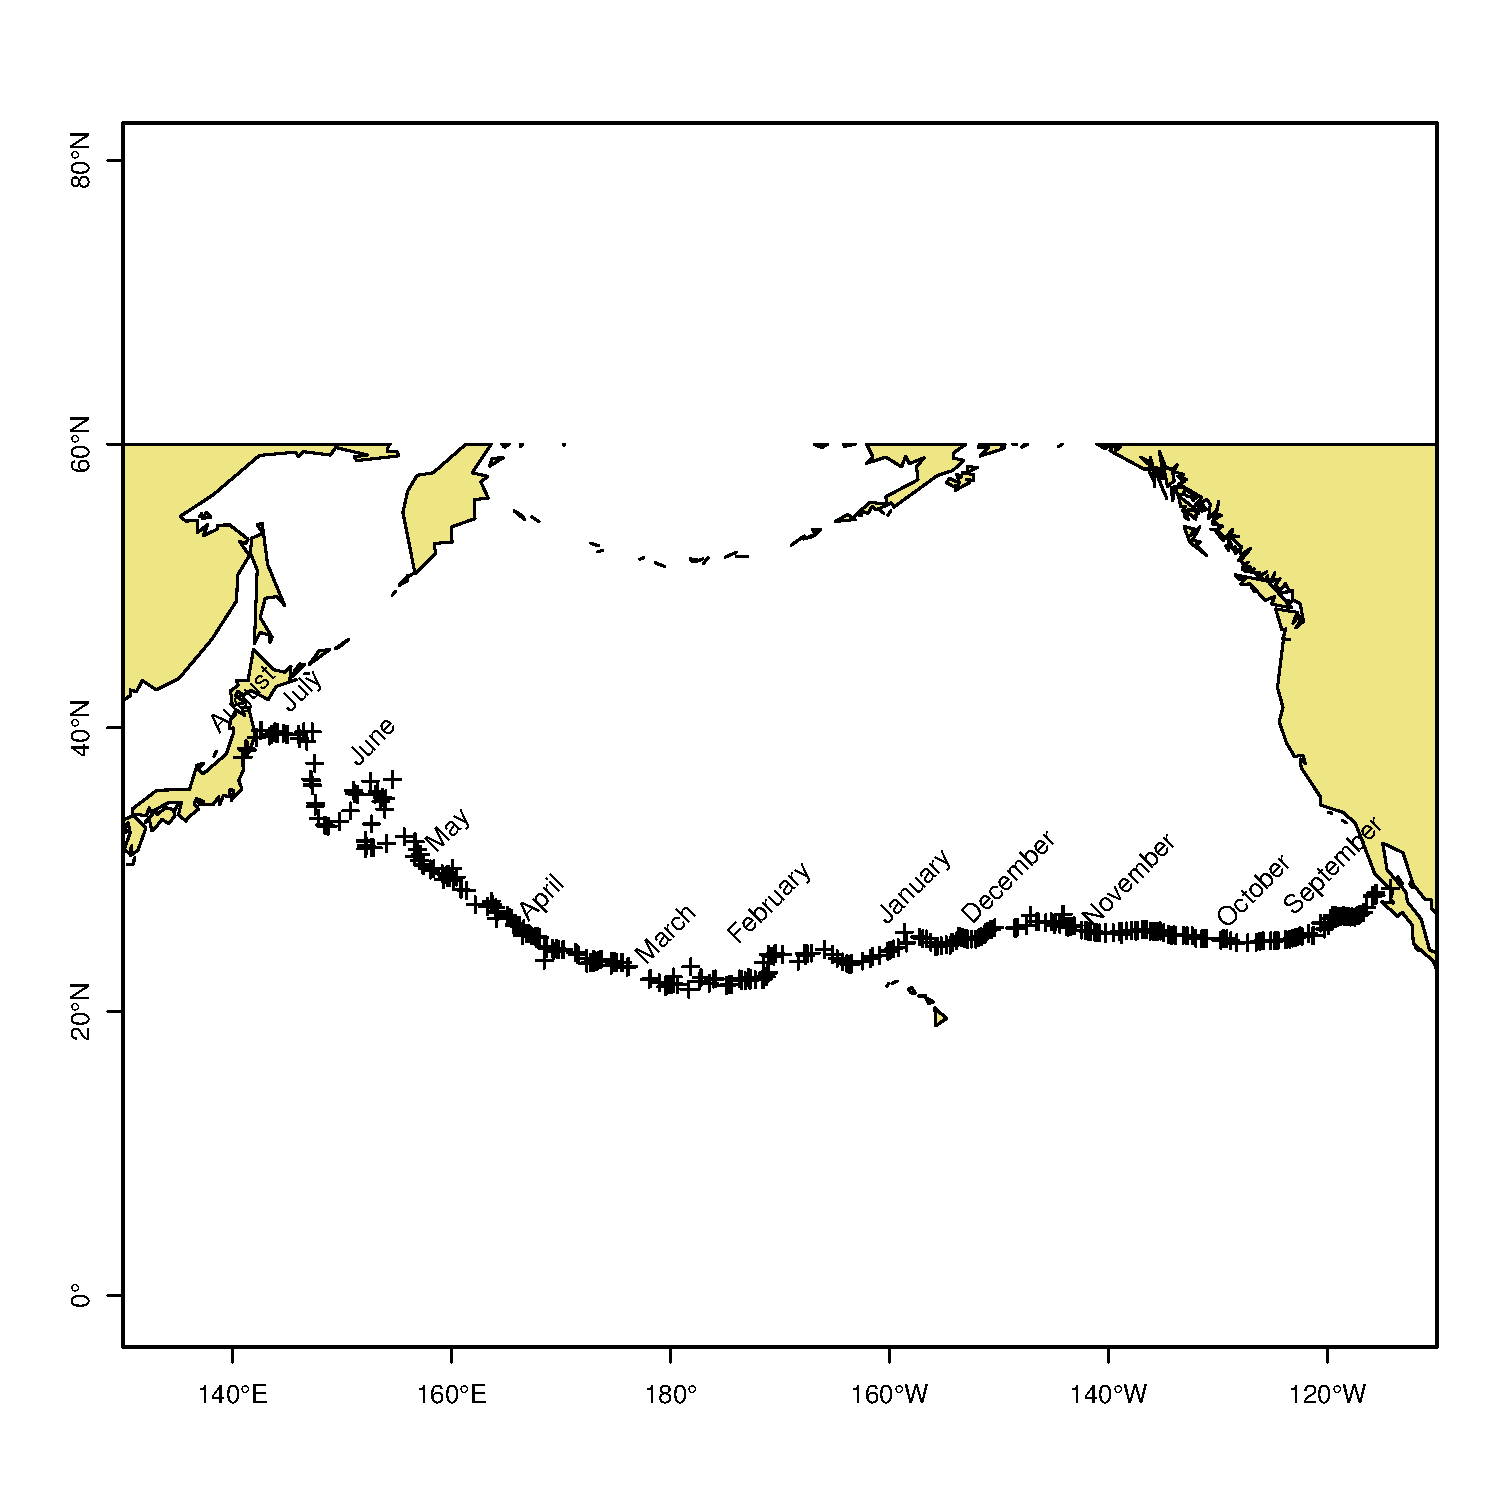
\includegraphics[width=0.7\columnwidth]{spatial_points_example.pdf}
% \end{minipage}
% \end{overlayarea}
% \end{frame}

% \subsubsection{空间线类}
% \begin{frame}[t,fragile]{\subsecname}{\subsubsecname}
% \begin{itemize}
% \item<1-> GIS中线对象是点对象的集合,在sp包中用\emphText{Line}类来表达;
% 而Line的集合又构成\emphText{Lines}类,其中不同Line通过NA值来区分
% \item<2-> 但是Line和Lines不包含约束盒和坐标系统,所以sp包提供\emphText{SpatialLines}类用来专门表达空间线对象
% \item<2-> SpatialLines类继承自Spatial类,除bbox和CRS之外,
% 还扩展了一个list类型的属性\emphText{lines}用来存储Lines对象
% \end{itemize}

% \begin{overlayarea}{\textwidth}{\textheight}
% \begin{onlyenv}<1>
% \begin{rcode}
% % # Line类包含属性coords用来存储构成线的连续点坐标矩阵
% > getClass("Line")
% Class "Line" [package "sp"]

% Slots:
             
% Name:  |\colorbox{green}{coords}|
% Class: matrix

% Known Subclasses: "Polygon"

% # Lines类包含一个属性Lines用来存储一系列Line对象,另一个属性ID用来标识Line对象的唯一性
% > getClass("Lines")
% Class "Lines" [package "sp"]

% Slots:
                          
% Name:      |\colorbox{green}{Lines}|        |\colorbox{green}{ID}|
% Class:      list character
% \end{rcode}
% \end{onlyenv}

% \begin{onlyenv}<2>
% \begin{rcode}
% % > getClass("SpatialLines")
% Class "SpatialLines" [package "sp"]

% Slots:
                                          
% Name:        |\colorbox{green}{lines}|        bbox proj4string
% Class:        list      matrix         CRS

% Extends: "Spatial"

% Known Subclasses: "SpatialLinesDataFrame"
% \end{rcode}
% \end{onlyenv}

% \begin{onlyenv}<3>
% \begin{rcode}
% % > library(maps)
% # 获取中国地图
% > china<- map("world", "china", plot=FALSE)
% # 台湾是中国领土不可分割的一部分!
% > tw <- map("world","taiwan",plot=FALSE)
% > china$x <- c(china$x,NA,tw$x)
% > china$y <- c(china$y,NA,tw$y)
% > china$range <- c(range(china$range[1:2],tw$range[1:2]),range(china$range[3:4],tw$range[3:4]))
% > china$names <- c(china$names,tw$names)
% > p4s <- CRS("+proj=longlat +ellps=WGS84")
% > library(maptools)
% # 用map2SpatialLines将地图数据转换为SpatialLines对象
% > SLchina <- |\colorbox{green}{map2SpatialLines}|(china,proj4string=p4s)
% > str(SLchina, max.level=2)
% Formal class 'SpatialLines' [package "sp"] with 3 slots
%   ..@ lines      :List of 41  # 由41个line对象组成
%   ..@ bbox       : num [1:2, 1:2] 73.6 18.2 134.8 53.6
%   .. ..- attr(*, "dimnames")=List of 2
%   ..@ proj4string:Formal class 'CRS' [package "sp"] with 1 slot
% \end{rcode}
% \end{onlyenv}

% \begin{onlyenv}<4>
% \begin{figure}[ht] \vspace{-15pt}
%   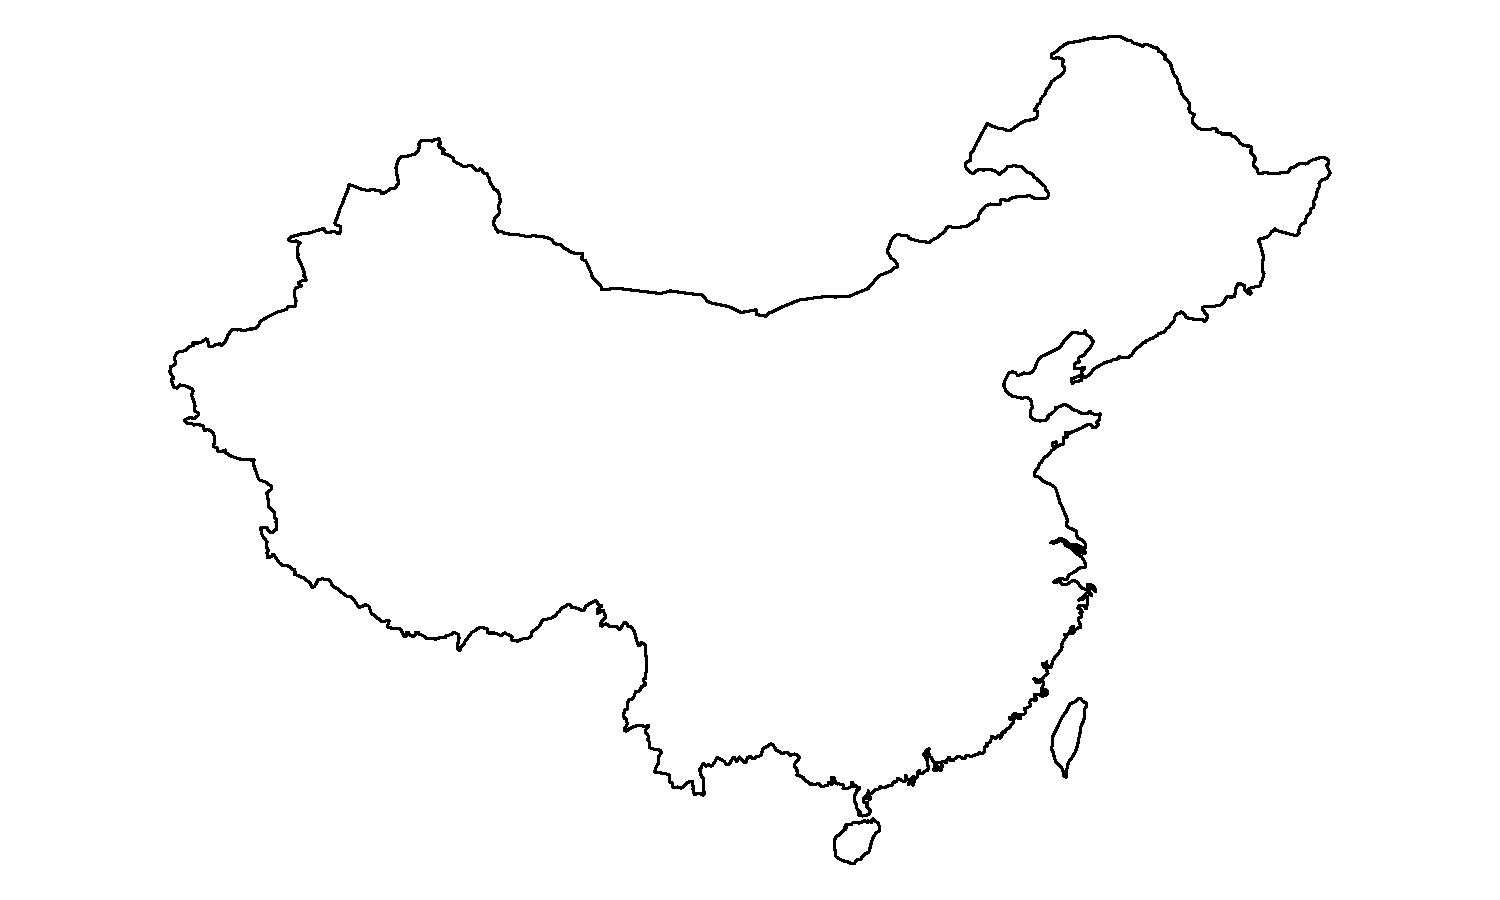
\includegraphics[width=0.8\columnwidth]{spatial_lines_example1.pdf}
% \end{figure}
% \end{onlyenv}
% \end{overlayarea}
% \end{frame}

% \begin{frame}[t,fragile]{\subsecname}{\subsubsecname}
% \begin{itemize}
% \item<1-> 类似空间点,sp包提供\emphText{SpatialLinesDataFrame}类将SpatialLines对象转换为类似data.frame数据结构,用于挂载属性数据
% \end{itemize}

% \begin{overlayarea}{\textwidth}{\textheight}
% \begin{onlyenv}<1>
% \begin{rcode}
% % > getClass("SpatialLinesDataFrame")
% Class "SpatialLinesDataFrame" [package "sp"]

% Slots:
                                                      
% Name:         data       lines        bbox proj4string
% Class:  data.frame        list      matrix         CRS

% Extends: 
% Class "SpatialLines", directly
% Class "Spatial", by class "SpatialLines", distance 2
% \end{rcode}
% \begin{figure}[ht] 
%   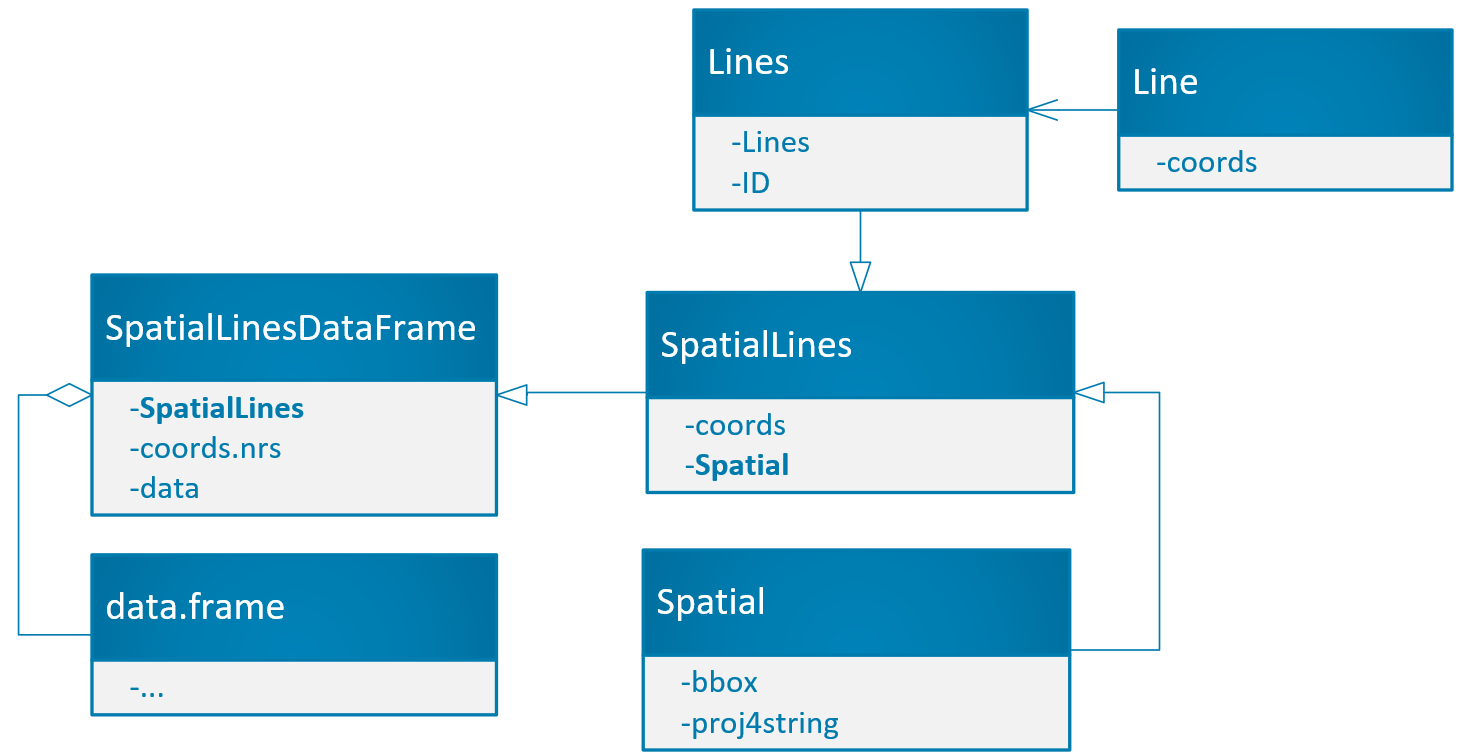
\includegraphics[width=0.7\columnwidth]{spatiallinesdataframe_class.png}
% \end{figure}
% \end{onlyenv}

% \begin{onlyenv}<2>
% \begin{rcode}
% % # maptools包中的ContourLines2SLDF函数将contourLines返回值转换为SpatialLinesDataFrame对象
% > volcano_sl <- ContourLines2SLDF(contourLines(volcano))
% # volcano\_sl的data slot包含10个不同的等高线水平标签
% > t(volcano_sl@data)
%       C_1   C_2   C_3   C_4   C_5   C_6   C_7   C_8   C_9   C_10 
% level "100" "110" "120" "130" "140" "150" "160" "170" "180" "190"
% \end{rcode}
% \begin{figure}[ht] \vspace{-10pt}
%   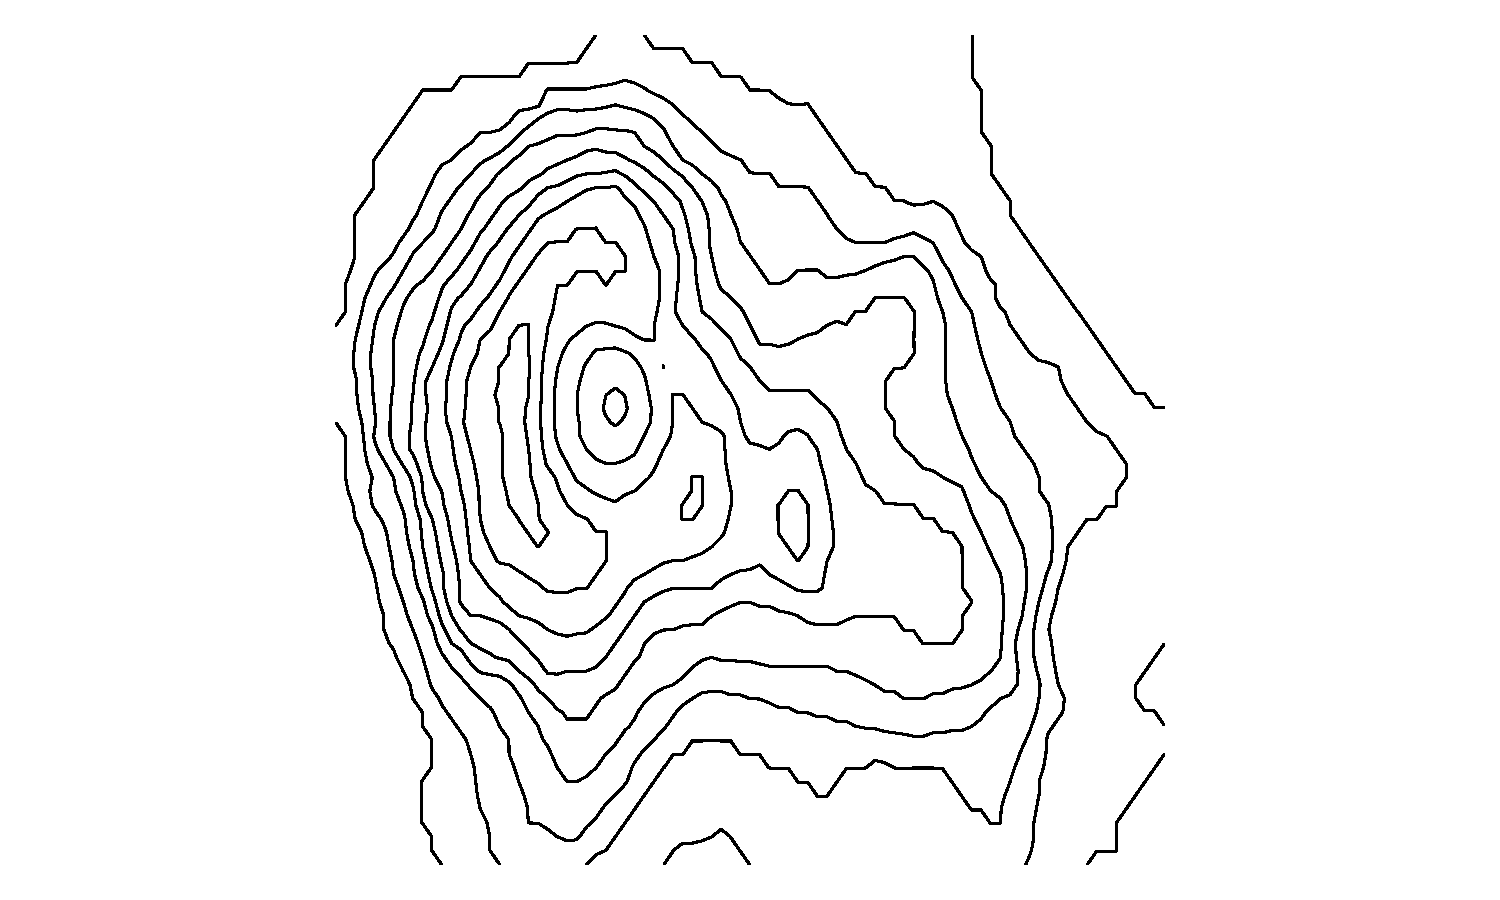
\includegraphics[width=0.8\columnwidth]{spatial_lines_example2.pdf}
% \end{figure}
% \end{onlyenv}
% \end{overlayarea}
% \end{frame}

% \subsubsection{空间面类}
% \begin{frame}[t,fragile]{\subsecname}{\subsubsecname}
% \begin{itemize}
% \item<1-> 在GIS中面是一个封闭的环(ring),用起始和终止坐标相同的点集存储,sp包定义\emphText{Polygon}类来表示面;一系列面对象构成\emphText{Polygons}类,其中不同Polygon通过NA值来区分
% \item<2-> 在面对象基础上,sp包继承Spatial类定义\emphText{SpatialPolygons}类来表达空间面对象,使其具有bbox和CRS
% \end{itemize}

% \begin{overlayarea}{\textwidth}{\textheight}
% \begin{onlyenv}<1>
% \begin{rcode}
% % # Polygon类包含属性coords用来存储起始和终止坐标相同的点坐标矩阵
% > getClass("Polygon")
% Class "Polygon" [package "sp"]

% Slots:
                                              
% Name:    labpt    area    hole ringDir  |\colorbox{green}{coords}|
% Class: numeric numeric logical integer  matrix

% Extends: "Line"

% # Polygons类包含一个属性Polygons用来存储一系列Polygon对象,另一个属性ID用来标识Polygon对象的唯一性
% > getClass("Polygons")
% Class "Polygons" [package "sp"]

% Slots:
                                                        
% Name:   Polygons plotOrder     labpt        ID      area
% Class:      list   integer   numeric character   numeric
% \end{rcode}
% \end{onlyenv}

% \begin{onlyenv}<2>
% \begin{rcode}
% % > getClass("SpatialPolygons")
% Class "SpatialPolygons" [package "sp"]

% Slots:
                                                      
% Name:     polygons   plotOrder        bbox proj4string
% Class:        list     integer      matrix         CRS

% Extends: "Spatial", "SpatialPolygonsNULL"

% Known Subclasses: 
% Class "SpatialPolygonsDataFrame", directly, with explicit coerce
% \end{rcode}
% \end{onlyenv}
% \end{overlayarea}
% \end{frame}

% \begin{frame}[t,fragile]{\subsecname}{\subsubsecname}
% \begin{itemize}
% \item<1-> sp包提供\emphText{SpatialPolygonsDataFrame}类将SpatialPolygons对象转换为类似data.frame数据结构,用于挂载属性数据
% \end{itemize}

% \begin{overlayarea}{\textwidth}{\textheight}
% \begin{onlyenv}<1>
% \begin{rcode}
% % > getClass("SpatialPolygonsDataFrame")
% Class "SpatialPolygonsDataFrame" [package "sp"]

% Slots:
                                                                  
% Name:         data    polygons   plotOrder        bbox proj4string
% Class:  data.frame        list     integer      matrix         CRS

% Extends: 
% Class "SpatialPolygons", directly
% Class "Spatial", by class "SpatialPolygons", distance 2
% Class "SpatialPolygonsNULL", by class "SpatialPolygons", distance 2, with explicit coerce
% \end{rcode}
% \begin{figure}[ht] \vspace{-10pt}
%   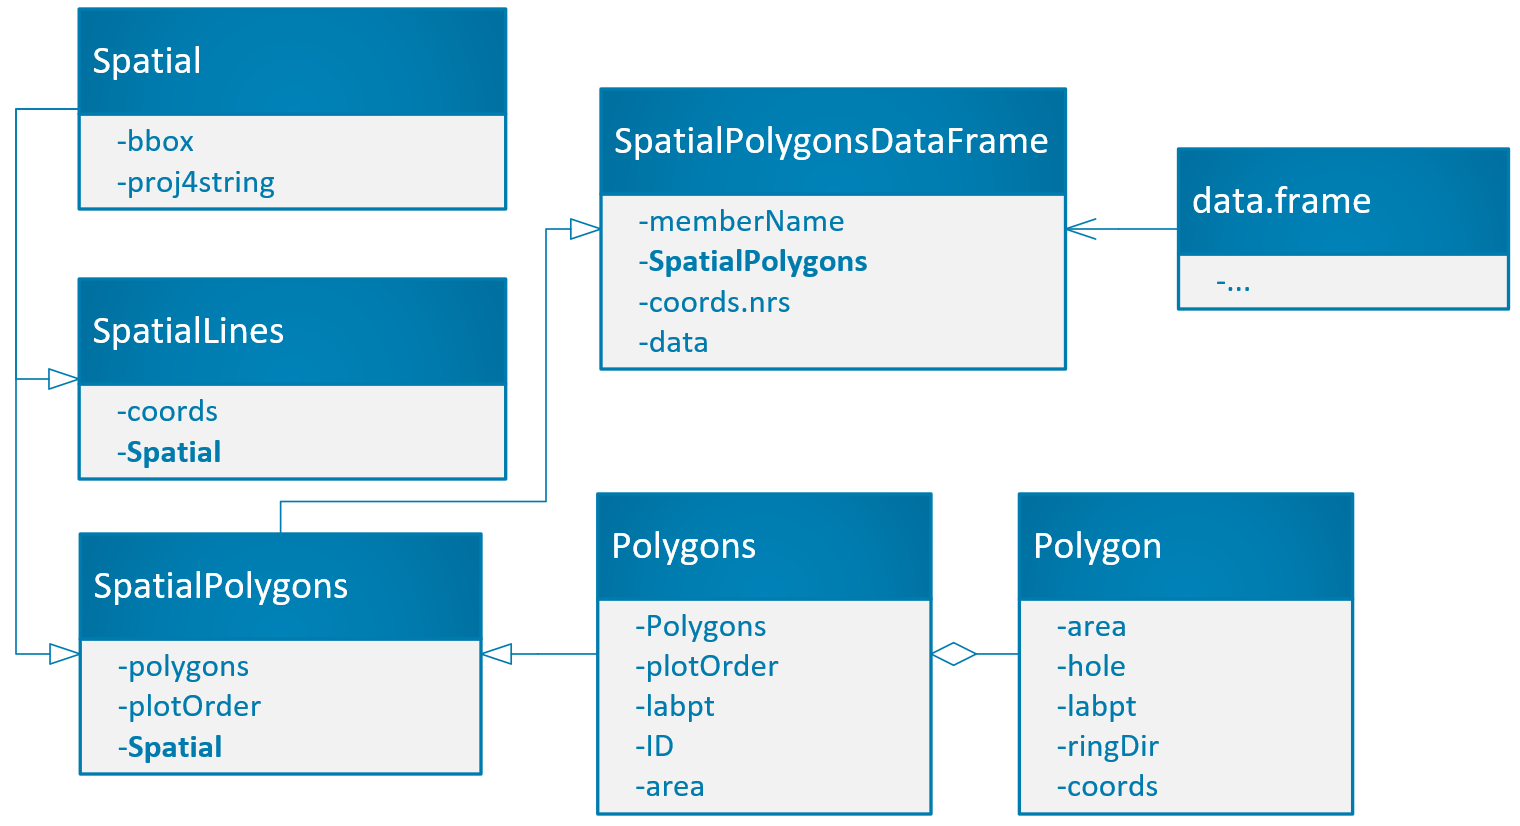
\includegraphics[width=0.7\columnwidth]{spatialpolygonsdataframe_class.png}
% \end{figure}
% \end{onlyenv}

% \begin{onlyenv}<2>
% \begin{rcode}
% % # 从maps包中读取美国州边界地图
% > library(maps)
% > state.map <- map("state", plot=FALSE, fill=TRUE)
% > IDs <- sapply(strsplit(state.map$names, ":"), function(x) x[1])
% > library(maptools)
% > state.sp <- map2SpatialPolygons(state.map, IDs=IDs,
%       proj4string=CRS("+proj=longlat +ellps=WGS84"))

% # 读取属性数据文件
% > sat <- read.table("data/state.sat.data_mod.txt", row.names=5, header=TRUE)
% # 属性数据包括四个字段
% > str(sat)
% 'data.frame':   52 obs. of  4 variables:
%  $ oname : Factor w/ 52 levels "ala","alaska",..: 1 2 3 4 5 6 7 9 8 10 ...
%  $ vscore: int  561 516 524 563 497 536 510 503 494 499 ...
%  $ mscore: int  555 514 525 556 514 540 509 497 478 498 ...
%  $ pc    : int  9 50 34 6 49 32 80 67 77 53 ...
% # 为属性数据添加ID字段,用于和空间对象进行关联
% > id <- match(row.names(sat), row.names(state.sp))
% > row.names(sat)[is.na(id)]
% > sat1 <- sat[!is.na(id),]
% # 创建SpatialPolygonsDataFrame对象
% > state.spdf <- SpatialPolygonsDataFrame(state.sp, sat1)
% > str(state.spdf, max.level=2)
% Formal class 'SpatialPolygonsDataFrame' [package "sp"] with 5 slots
%   ..@ data       :'data.frame': 49 obs. of  4 variables:
%   ..@ polygons   :List of 49
%   ..@ plotOrder  : int [1:49] 42 25 4 30 27 2 5 49 36 22 ...
%   ..@ bbox       : num [1:2, 1:2] -124.7 25.1 -67 49.4
%   .. ..- attr(*, "dimnames")=List of 2
%   ..@ proj4string:Formal class 'CRS' [package "sp"] with 1 slot
% \end{rcode}
% \end{onlyenv}

% \begin{onlyenv}<3> \centering
% \begin{columns} 
%     \begin{column}{.4\textwidth} 
%         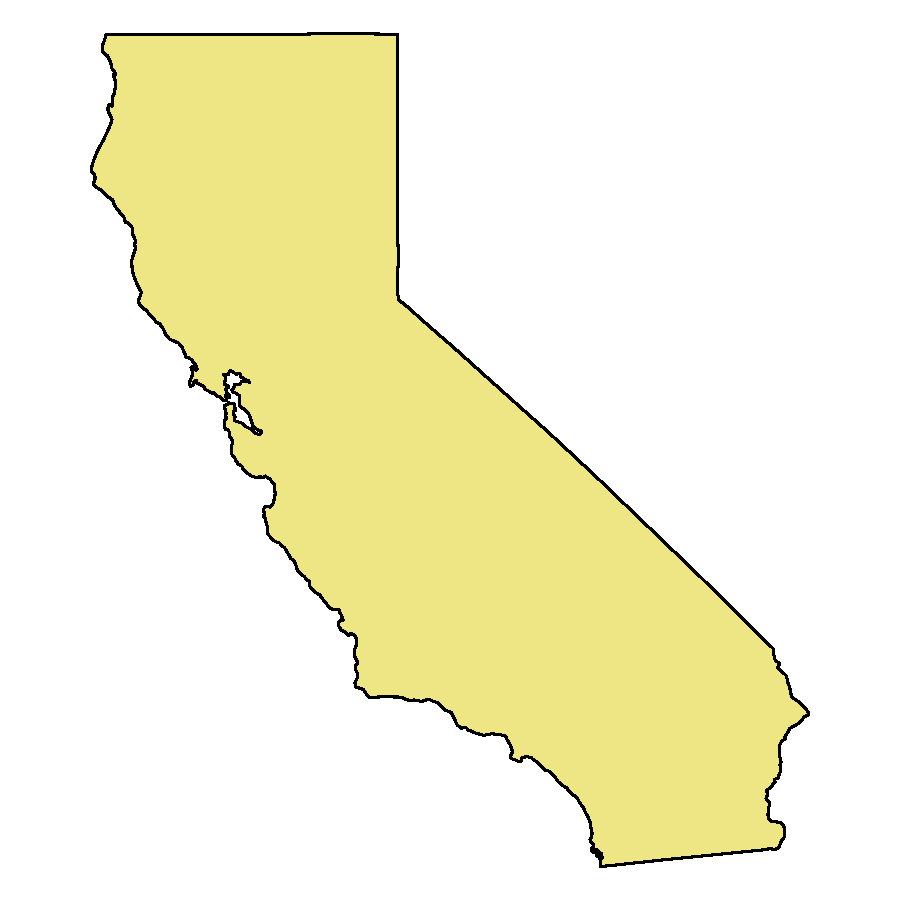
\includegraphics[width=\columnwidth]{spatial_polygons_example1.pdf}
%     \end{column}

%     \begin{column}{.6\textwidth}
% \begin{rcode} 
% % # 从SpatialPolygonsDataFrame对象中取得特定的数据
% > california <- state.spdf[state.spdf$oname== "calif",]
% > str(california,max.level=2)
% Formal class 'SpatialPolygonsDataFrame' [package "sp"] with 5 slots
%   ..@ data       :'data.frame': 1 obs. of  4 variables:
%   ..@ polygons   :List of 1
%   ..@ plotOrder  : int 1
%   ..@ bbox       : num [1:2, 1:2] -124.4 32.5 -114.1 42
%   .. ..- attr(*, "dimnames")=List of 2
%   ..@ proj4string:Formal class 'CRS' [package "sp"] with 1 slot
% > california@data
%            oname vscore mscore pc
% california calif    497    514 49
% \end{rcode}
%     \end{column}
%   \end{columns}
% \end{onlyenv}
% \end{overlayarea}
% \end{frame}

% \begin{frame}[t,fragile]{\subsecname}{\subsubsecname}
% \begin{itemize}
% \item<1-> 在地理实体中,除了岛(island)这种简单的面对象之外,还存在洞(hole)这种特殊的面对象,在sp包中
% 简单通过\emphText{逻辑标记hole}定义面对象是否是洞
% \item<1-> 如果hole没有指定,那么可以通过\emphText{ringDir}属性来判定环的方向,1表示顺时针则是岛,-1表示逆时针是洞
% \item<3-> Polygons类的\emphText{plotOrder}属性用来处理复杂面集合的绘制顺序
% \end{itemize}

% \begin{overlayarea}{\textwidth}{\textheight}
% \begin{onlyenv}<1>
% \begin{rcode}
% > getClass("Polygon")
% Class "Polygon" [package "sp"]

% Slots:
                                              
% Name:    labpt    area    |\colorbox{green}{hole}| |\colorbox{green}{ringDir}|  coords
% Class: numeric numeric logical integer  matrix

% Extends: "Line"
% > getClass("Polygons")
% Class "Polygons" [package "sp"]

% Slots:
                                                        
% Name:   Polygons |\colorbox{green}{plotOrder}     labpt        ID      area
% Class:      list   integer   numeric character   numeric
% \end{rcode}
% \end{onlyenv}

% \begin{onlyenv}<2>
% \begin{rcode}
% # 加载一个包含洞对象和岛对象的数据
% > load("data/high.RData")
% > manitoulin_sp <- high$SP
% # 数据只有一个Polygons
% > length(manitoulin_sp@polygons)
% > 1
% # Polygons中包含19个Polygon
% > str(manitoulin_sp@polygons[[1]],max.level=2)
% Formal class 'Polygons' [package "sp"] with 5 slots
%   ..@ Polygons :List of 19
%   ..@ plotOrder: int [1:19] 1 2 3 4 18 17 19 5 6 7 ...
%   ..@ labpt    : num [1:2] 278 46
%   ..@ ID       : chr "2"
%   ..@ area     : num 0.694
% # 19个Polygon中有4个洞,15个岛
% > sapply(manitoulin_sp@polygons[[1]]@Polygons, function(x) slot(x, "hole"))
%  [1] FALSE  TRUE FALSE FALSE FALSE FALSE FALSE FALSE FALSE FALSE FALSE FALSE
% [13] FALSE FALSE FALSE FALSE  TRUE  TRUE  TRUE
% > sapply(manitoulin_sp@polygons[[1]]@Polygons, function(x) slot(x, "ringDir"))
%  [1]  1 -1  1  1  1  1  1  1  1  1  1  1  1  1  1  1 -1 -1 -1
% \end{rcode}
% \end{onlyenv}

% \begin{onlyenv}<3>
% \begin{figure}[ht] \vspace{-20pt}
%   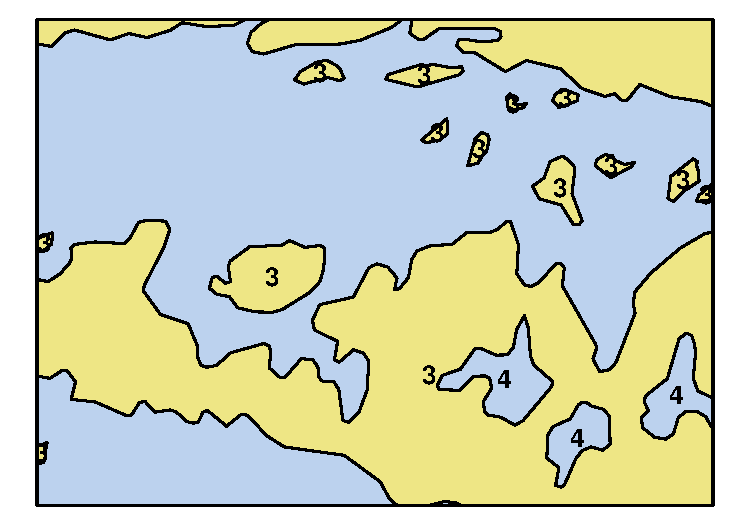
\includegraphics[width=0.6\columnwidth]{spatial_polygons_example2.pdf}
%   \caption{先绘制大陆,接着是湖,然后是岛,最后是岛上的湖}
% \end{figure}
% \end{onlyenv}
% \end{overlayarea}
% \end{frame}

% \subsubsection{栅格数据类}
% \begin{frame}[t,fragile]{\subsecname}{\subsubsecname}
% \begin{itemize}
% \item<1-> sp包除了矢量数据,还提供了SpatialGrid类和SpatialPixel类用于表达栅格数据
% \item<2-> \emphText{GridTopology}类用于表达基本的网格对象,\emphText{SpatialGrid}类在此基础上继承了Spatial类,使其具有bbox和CRS属性
% \end{itemize}

% \begin{overlayarea}{\textwidth}{\textheight}
% \begin{onlyenv}<2>
% \begin{rcode}
% # 通过左下角网格中心点坐标、网格尺寸和网格数目三个属性来定义基本网格
% > getClass("GridTopology")
% Class "GridTopology" [package "sp"]

% Slots:
                                                            
% Name:  |\colorbox{green}{cellcentre.offset}|          |\colorbox{green}{cellsize}|         |\colorbox{green}{cells.dim}|
% Class:           numeric           numeric           integer
% # 定义一个bbox范围
% > b <- bbox(manitoulin_sp)
% > bb
%     min   max
% x 277.0 278.0
% y  45.7  46.2
% # 定义左小角中心点坐标和网格尺寸
% > cs <- c(0.01, 0.01)
% > cc <- bb[,1]+(cs/2)
% # 定义x和y两个方向的网格数目
% > cd <- ceiling(diff(t(bb))/cs)
% # 创建一个GridTopology对象
% > manitoulin_grd <- GridTopology(cellcentre.offset=cc, cellsize=cs, cells.dim=cd)
% > manitoulin_grd
%                         x      y
% cellcentre.offset 277.005 45.705
% cellsize            0.010  0.010
% cells.dim         100.000 50.000
% \end{rcode}
% \end{onlyenv}

% \begin{onlyenv}<3>
% \begin{rcode}
% > getClass("SpatialGrid")
% Class "SpatialGrid" [package "sp"]

% Slots:
                                             
% Name:          grid         bbox  proj4string
% Class: GridTopology       matrix          CRS

% Extends: "Spatial"

% Known Subclasses: "SpatialGridDataFrame"
% > p4s <- CRS(proj4string(manitoulin_sp))
% # 创建SpatialGrid对象
% > manitoulin_SG <- SpatialGrid(manitoulin_grd, proj4string=p4s)
% > summary(manitoulin_SG)
% Object of class SpatialGrid
% Coordinates:
%     min   max
% x 277.0 278.0
% y  45.7  46.2
% Is projected: FALSE 
% proj4string :
% [+proj=longlat +datum=WGS84 +ellps=WGS84 +towgs84=0,0,0]
% Grid attributes:
%   cellcentre.offset cellsize cells.dim
% x           277.005     0.01       100
% y            45.705     0.01        50
% \end{rcode}
% \end{onlyenv}

% \begin{onlyenv}<4>
% \begin{figure}[ht] \vspace{-10pt}
%   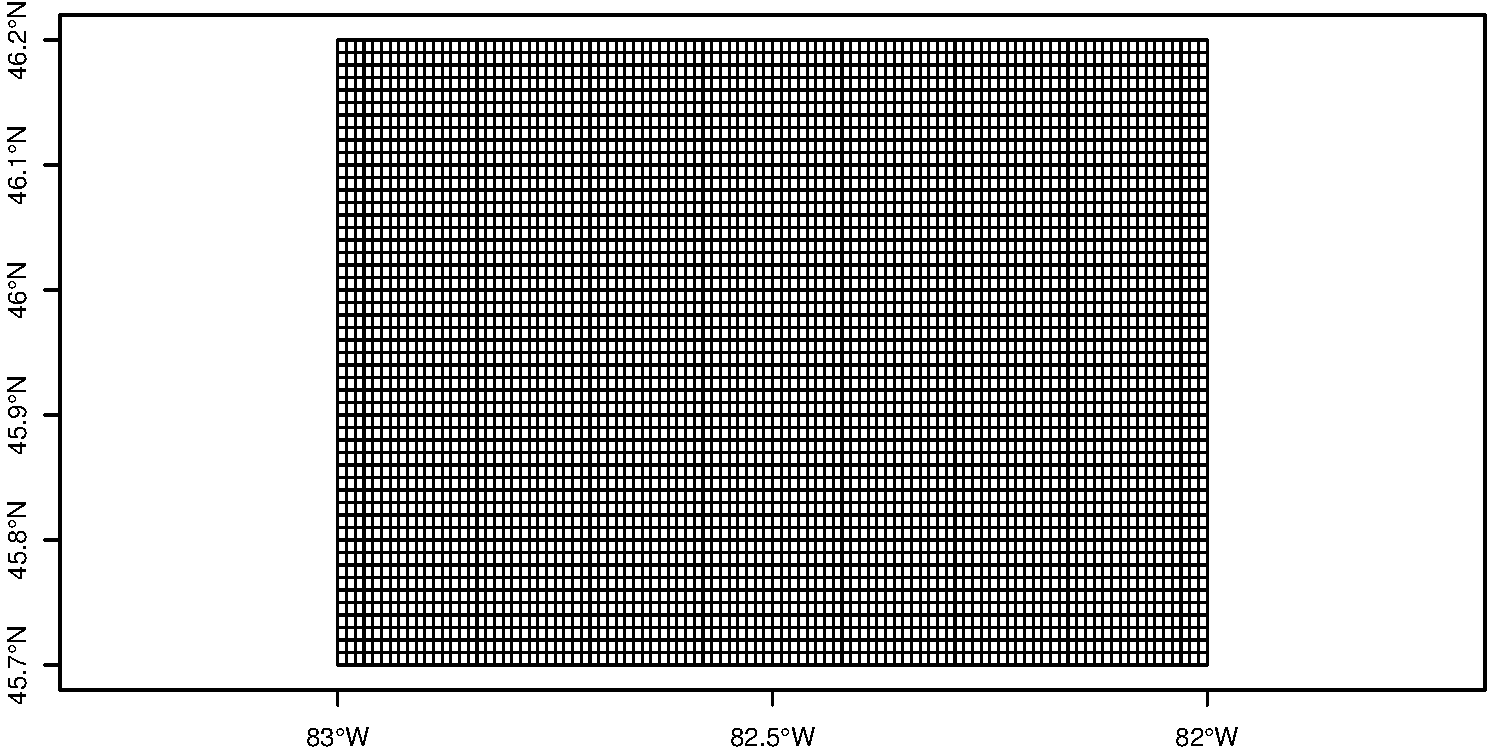
\includegraphics[width=\columnwidth]{spatial_grid_example1.pdf}
% \end{figure}
% \end{onlyenv}
% \end{overlayarea}
% \end{frame}

% \begin{frame}[t,fragile]{\subsecname}{\subsubsecname}
% \begin{itemize}
% \item<1-> sp包提供\emphText{SpatialGridDataFrame}类将SpatialGrid对象转换为类似data.frame数据结构,用于挂载网格上的属性,例如高程、温度、风力、颜色等
% \item<1-> SpatialGridDataFrame类的data属性\emphText{存储完整网格的全部属性数据},包括NA值的
% \end{itemize}

% \begin{overlayarea}{\textwidth}{\textheight}
% \begin{onlyenv}<1>
% \begin{rcode}
% # 读取一个Geotiff格式栅格数据数据到SpatialGridDataFrame对象auck\_el1
% > library(rgdal)
% > auck_el1 <- readGDAL("data/70042108.tif")
% # 对象是由1320*1200的维度构成
% > auck_el1@grid
%                              x             y
% cellcentre.offset 1.742004e+02 -3.749958e+01
% cellsize          8.333333e-04  8.333333e-04
% cells.dim         1.320000e+03  1.200000e+03
% # data存储了完整的1584000个网格的属性数据
% > str(auck_el1,max.level=2)
% Formal class 'SpatialGridDataFrame' [package "sp"] with 4 slots
%   ..@ data       :'data.frame': 1584000 obs. of  1 variable:
%   ..@ grid       :Formal class 'GridTopology' [package "sp"] with 3 slots
%   ..@ bbox       : num [1:2, 1:2] 174.2 -37.5 175.3 -36.5
%   .. ..- attr(*, "dimnames")=List of 2
%   ..@ proj4string:Formal class 'CRS' [package "sp"] with 1 slot
% # data属性只有一个band1字段,表示海拔高程;将高程等于或者小于0米的网格设置为NA
% > str(auck_el1@data)
% 'data.frame':   1584000 obs. of  1 variable:
%  $ band1: num  40 45 42 34 42 59 79 99 113 127 ... 
% > is.na(auck_el1$band1) <- auck_el1$band1 <= 0
% > summary(auck_el1$band1)
%    Min. 1st Qu.  Median    Mean 3rd Qu.    Max.    NA's 
%     1.0    23.0    53.0    78.1   106.0   686.0  791938 
% \end{rcode}
% \end{onlyenv}
% \end{overlayarea}
% \end{frame}

% \begin{frame}[t,fragile]{\subsecname}{\subsubsecname}
% \begin{itemize}
% \item<1-> sp包还提供了\emphText{SpatialPixels}类实现另一种栅格数据表达;与SpatialGrid相比,SpatialPixels
% 增加了\emphText{grid.index}和\emphText{coords}属性,分别用于存储网格索引和中心点坐标
% \item<2-> 一个好处是在\emphText{SpatialPixelsDataFrame}类中\emphText{只存储非NA值的网格属性},
% 可以减小data属性的存储空间和处理时间
% \item<2-> 另一个好处是可以\emphText{将栅格数据以空间点存储在外部数据库中},也可以由空间点类创建栅格数据
% \end{itemize}

% \begin{overlayarea}{\textwidth}{\textheight}
% \begin{onlyenv}<1>
% \begin{rcode}
% > getClass("SpatialPixels")
% Class "SpatialPixels" [package "sp"]

% Slots:
                                                                       
% Name:          grid   |\colorbox{green}{grid.index}|       |\colorbox{green}{coords}|         bbox  proj4string
% Class: GridTopology      integer       matrix       matrix          CRS

% Extends: 
% Class "SpatialPoints", directly
% Class "Spatial", by class "SpatialPoints", distance 2

% Known Subclasses: "SpatialPixelsDataFrame"
% \end{rcode}
% \end{onlyenv}

% \begin{onlyenv}<2>
% \begin{rcode}
% # 转换为SpatialPixelsDataFrame类
% > auck_el2 <- as(auck_el1, "SpatialPixelsDataFrame")
% # 由于data属性只存储非NA值,因此只有792062维度
% # grid.index属性用于网格索引,只存储非NA值网格的序号
% # coords属性可以和SpatialPoints类互相转换适合在外部数据库中存储
% > str(auck_el2, max.level=2)
% Formal class 'SpatialPixelsDataFrame' [package "sp"] with 7 slots
%   ..@ data       :'data.frame': 792062 obs. of  1 variable:
%   ..@ coords.nrs : num(0) 
%   ..@ grid       :Formal class 'GridTopology' [package "sp"] with 3 slots
%   ..@ |\colorbox{green}{grid.index}| : int [1:792062] 1 2 3 4 5 6 7 8 9 10 ...
%   ..@ |\colorbox{green}{coords}|     : num [1:792062, 1:2] 174 174 174 174 174 ...
%   .. ..- attr(*, "dimnames")=List of 2
%   ..@ bbox       : num [1:2, 1:2] 174.2 -37.5 175.3 -36.5
%   .. ..- attr(*, "dimnames")=List of 2
%   ..@ proj4string:Formal class 'CRS' [package "sp"] with 1 slot
% \end{rcode}
% \end{onlyenv}

% \begin{onlyenv}<3>
% \begin{rcode}
% # SpatialPixelsDataFrame减少了data属性存储空间
% > object.size(auck_el1@data)
% 12672672 bytes
% > object.size(auck_el2@data)
% 9505408 bytes

% # 虽然data不用存储NA值,但是SpatialPixelsDataFrame需要额外存储coords和gird.index,
% # 所以如果属性很少,而且非NA值比例不高的情况下,反而占的空间比较大
% > object.size(auck_el1) # SpatialGridDataFrame不用存储coords和grid.index
% 12676296 bytes
% > object.size(auck_el2@grid.index) # grid.index另外占用空间
% 3168288 bytes
% > object.size(auck_el2@coords) # coords另外占用空间
% 12673512 bytes
% # 占用空间几乎是SpatialGridDataFrame的二倍,但是在处理速度上由于有grid.index索引,
% # 因此比SpatialGridDataFrame要快
% > object.size(auck_el2) 
% 25351272 bytes
% \end{rcode}
% \end{onlyenv}

% \begin{onlyenv}<4>
% \begin{figure}[ht] \vspace{-20pt}
%   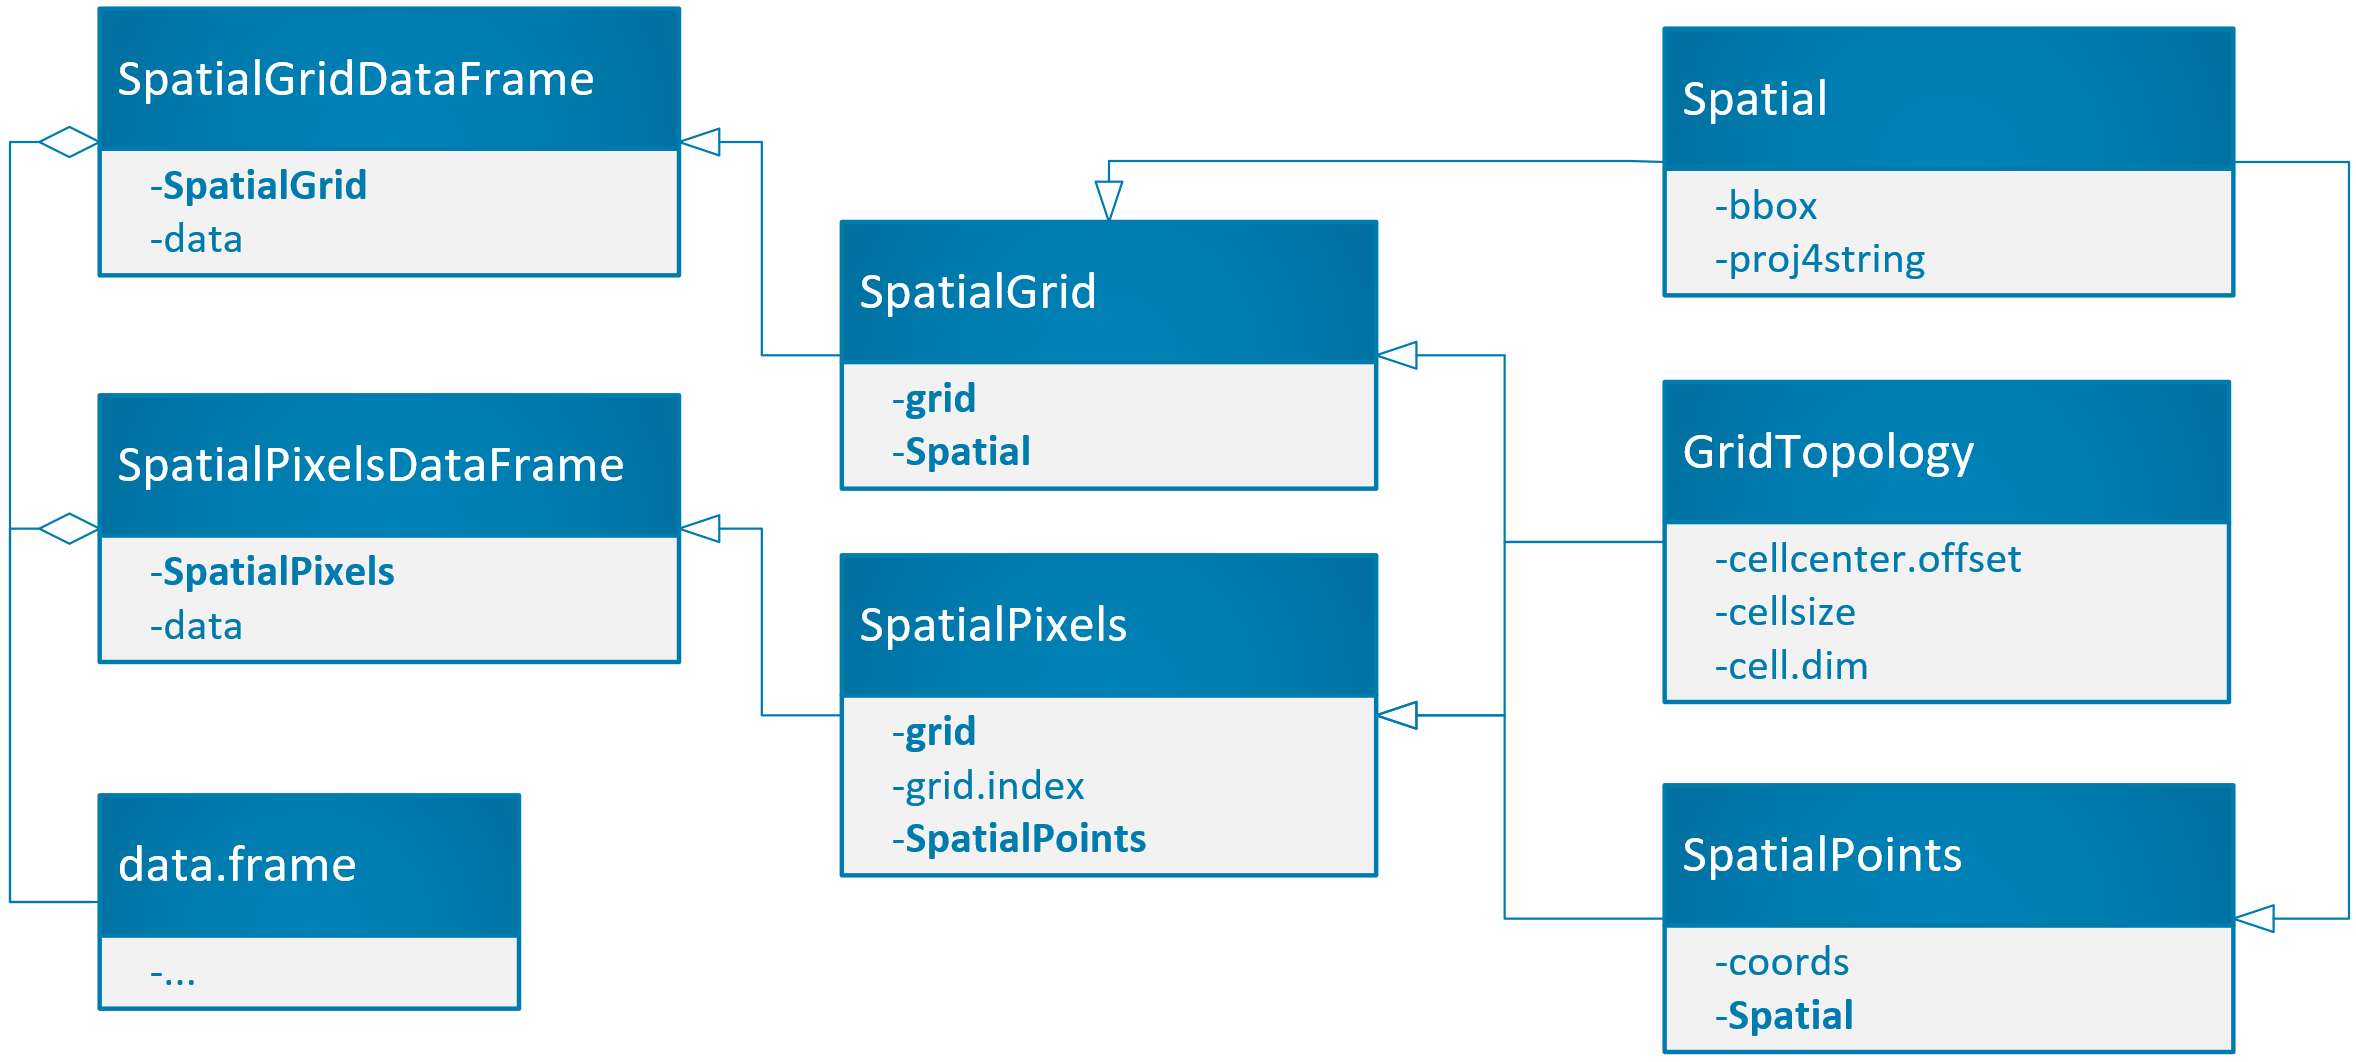
\includegraphics[width=\columnwidth]{spatialpixelsdataframe_class.png}
% \end{figure}
% \end{onlyenv}
% \end{overlayarea}
% \end{frame}

% \begin{frame}[t,fragile]{\subsecname}{\subsubsecname}
% \begin{itemize}
% \item<1-> sp包处理栅格数据的方式是将所有数据一次性读入内存,但是这样对于大数据量可能会导致内存溢出,因此
% 从2010年开始CRAN发布了\emphText{raster包},可以将栅格数据分块读入内存
% \item<2-> raster包提供\emphText{raster函数}值将参数读入内存创建\emphText{RasterLayer}对象,而并不读入网格数据;
% 当需要读取数据到内存时,则调用\emphText{getValues}或\emphText{extract}函数

% \end{itemize}

% \begin{overlayarea}{\textwidth}{\textheight}
% \begin{onlyenv}<2>
% \begin{rcode}
% > library(raster)
% # 读取栅格文件数据到RasterLayer对象
% > r <- raster("data/70042108.tif")
% # RasterLayer对象只存储数据的参数,包括维度、分辨率、范围、CRS、文件路径和名称
% > r
% class       : RasterLayer 
% dimensions  : 1200, 1320, 1584000  (nrow, ncol, ncell)
% resolution  : 0.0008333333, 0.0008333333  (x, y)
% extent      : 174.2, 175.3, -37.5, -36.5  (xmin, xmax, ymin, ymax)
% coord. ref. : +proj=longlat +datum=WGS84 +no_defs +ellps=WGS84 +towgs84=0,0,0 
% data source : /home/mono/Documents/tex_projects/r_guide_slide/data/70042108.tif 
% names       : X70042108
% # 并没有将网格数据读入内存,因此只占用很小的空间
% > inMemory(r)
% [1] FALSE
% > object.size(r)
% 12032 bytes
% # 用getValues函数将所有网格数据读入内存
% > rs <- getValues(r)
% > object.size(rs)
% 12672040 bytes
% \end{rcode}
% \end{onlyenv}
% \end{overlayarea}
% \end{frame}

% \begin{frame}[t,fragile]{\subsecname}{\subsubsecname}
% \begin{itemize}
% \item<1-> RasterLayer只能表达一个属性的栅格数据,而有多个属性时,则可以在相同的空间范围和分辨率网格中叠加存储数据,raster包提供了\emphText{brick}和\emphText{stack}两个函数来实现
% \item<2-> brick函数读入一个包含多层栅格数据的文件,而stack函数读入多个只包含一层栅格数据的文件;brick函数创建
% \emphText{RasterBrick}对象,而stack函数创建\emphText{RasterStack}对象
% \end{itemize}

% \begin{overlayarea}{\textwidth}{\textheight}
% \begin{onlyenv}<2>
% \begin{rcode}
% > library(raster)
% # 读取并创建一个RasterLayer对象
% > data <- system.file("external/test.grd", package="raster")
% > r1 <- raster(data) 
% > nlayers(r1)  # r1对象只包含一层数据,也就是一个属性
% [1] 1
% # 创建第二个RasterLayer对象
% > r2 <- r1 * r1
% # 创建第三个RasterLayer对象
% > r3 <- sqrt(r1)
% # 三个具有相同空间范围和分辨率的RasterLayer对象通过stack函数叠加后创建RasterStack对象
% > s <- |\colorbox{green}{stack}|(r1,r2,r3)
% > s # 创建的RasterStack对象包括三个数据层
% class       : RasterStack 
% dimensions  : 115, 80, 9200, 3  (nrow, ncol, ncell, nlayers)
% resolution  : 40, 40  (x, y)
% extent      : 178400, 181600, 329400, 334000  (xmin, xmax, ymin, ymax)
% coord. ref. : +init=epsg:28992 +towgs84=565.237,50.0087,465.658,-0.406857,0.350733,-1.87035,4.0812 +proj=sterea +lat_0=52.15616055555555 +lon_0=5.38763888888889 +k=0.9999079 +x_0=155000 +y_0=463000 +ellps=bessel +units=m +no_defs 
% names       :         |\colorbox{green}{test}|,      |\colorbox{green}{layer.1}|,      |\colorbox{green}{layer.2}| 
% min values  :    128.43401,  16495.29383,     11.33287 
% max values  : 1.805780e+03, 3.260842e+06, 4.249447e+01 
% \end{rcode}
% \end{onlyenv}

% \begin{onlyenv}<3>
% \begin{figure}[ht] 
%   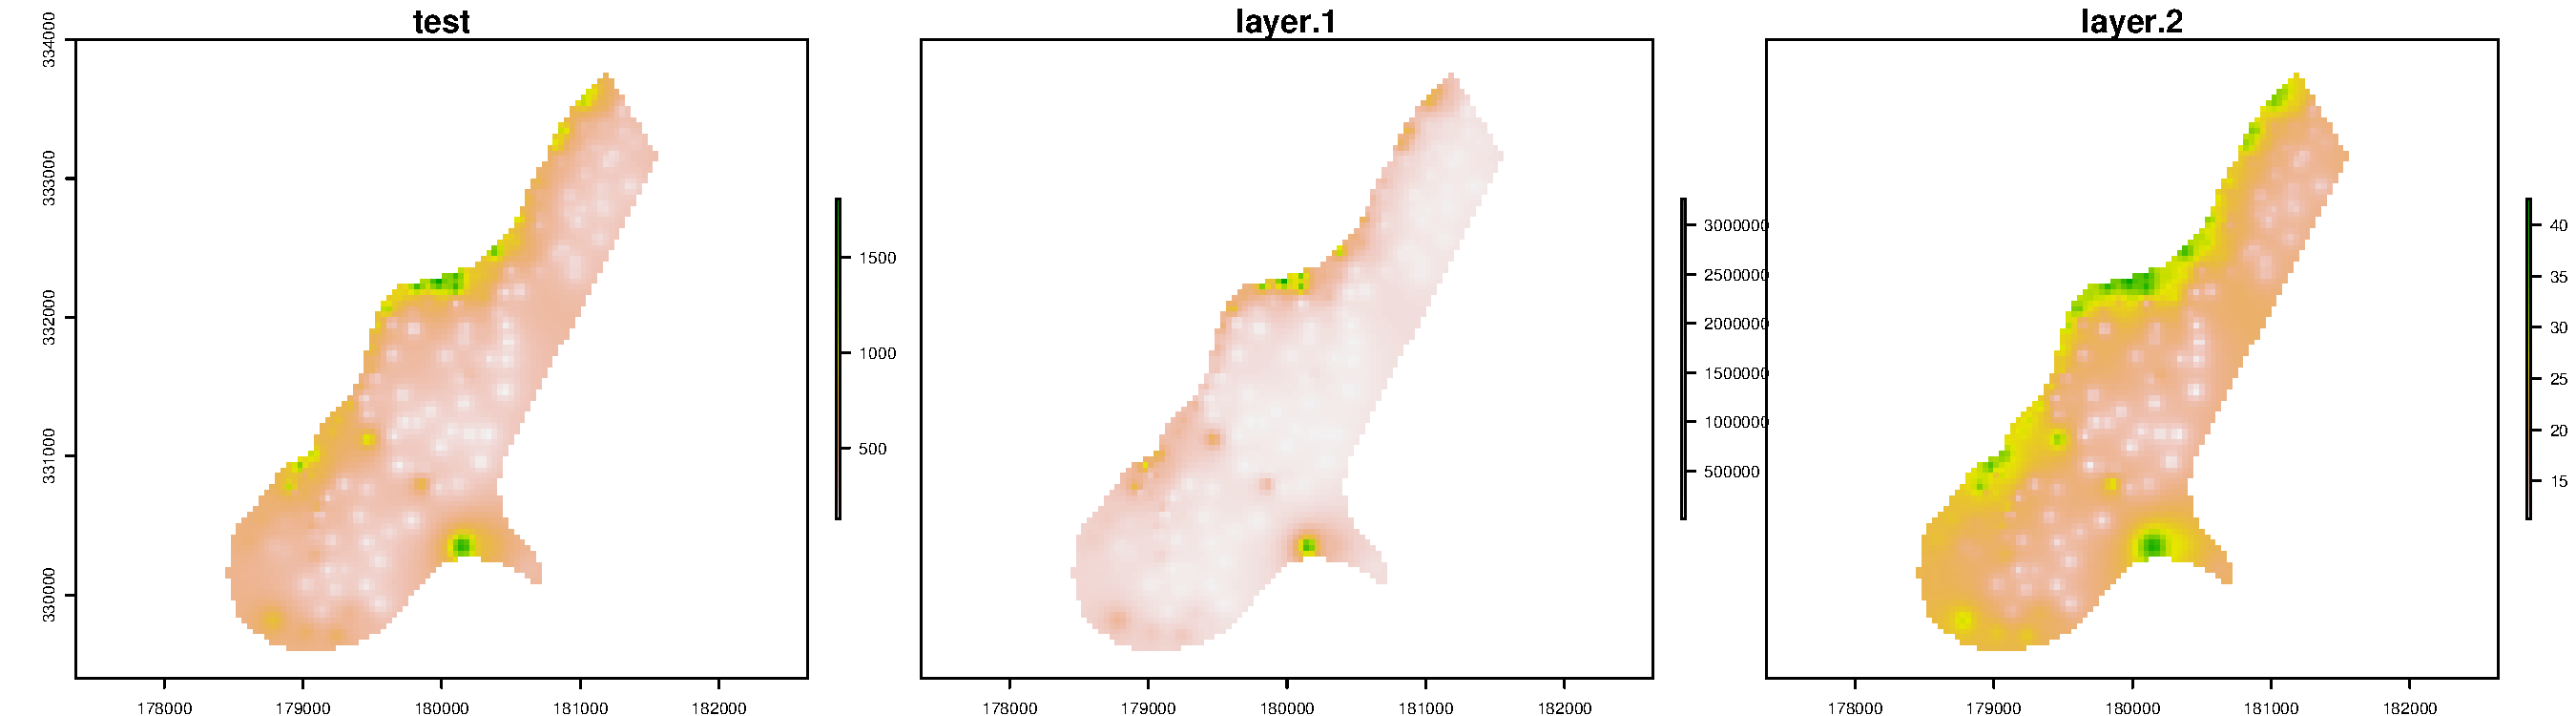
\includegraphics[width=\columnwidth]{spatial_raster_example1.pdf}
% \end{figure}
% \end{onlyenv}

% \begin{onlyenv}<4>
% \begin{rcode}
% # 读取一个包含多层数据的栅格文件
% > b <- |\colorbox{green}{brick}|(system.file("external/rlogo.grd", package="raster"))
% # brick函数创建的RasterBrick对象
% > b
% class       : RasterBrick 
% dimensions  : 77, 101, 7777, 3  (nrow, ncol, ncell, nlayers)
% resolution  : 1, 1  (x, y)
% extent      : 0, 101, 0, 77  (xmin, xmax, ymin, ymax)
% coord. ref. : +proj=merc +datum=WGS84 +ellps=WGS84 +towgs84=0,0,0 
% data source : /home/mono/Softwares/R/3.4/raster/external/rlogo.grd 
% names       : red, green, blue 
% min values  :   0,     0,    0 
% max values  : 255,   255,  255 
% # RasterBrick对象包含三层数据
% > nlayers(b)
% [1] 3
% # 三层数据对应的三个属性
% > names(b)
% [1] "red"   "green" "blue" 
% \end{rcode}
% \end{onlyenv}
% \end{overlayarea}
% \end{frame}

% \begin{frame}[t,fragile]{\subsecname}{\subsubsecname}
% \begin{itemize}
% \item<1-> raster包提供\emphText{blockSize}函数对栅格数据进行分块,分块按照整行读取,根据行数确定分块大小
% \item<1-> \emphText{writeValues}函数将分块数据写入文件,
% \emphText{writeStart}和\emphText{writeStop}函数则控制此写入过程的起始和终止
% \end{itemize}

% \begin{overlayarea}{\textwidth}{\textheight}
% \begin{onlyenv}<2>
% \begin{rcode}
% > out <- raster("data/70042108.tif")
% > bs <- |\colorbox{green}{blockSize}|(out)
% > bs # 默认分块数为4,row是每块起始的行号,nrows是每个分块的行数
% $row
% [1]   1 301 601 901
% $nrows
% [1] 300 300 300 300
% $n
% [1] 4
% # 开始写入操作,创建一个临时文件
% > out <- |\colorbox{green}{writeStart}|(out, filename=tempfile(), overwrite=TRUE)
% > for (i in 1:bs$n) {
% +     v <- getValues(r, row=bs$row[i], nrows=bs$nrows[i]) # 读取分块数据
% +     v[v <= 0] <- NA # 分块中高程小于或等于0米的数据设置为NA值
% +     |\colorbox{green}{writeValues}|(out, v, bs$row[i])} # 将分块数据写入临时文件
% # 结束写入操作,释放文件锁
% > out <- |\colorbox{green}{writeStop}|(out) 
% > out  # 从data source可以看到写入文件的位置
% class       : RasterLayer 
% dimensions  : 1200, 1320, 1584000  (nrow, ncol, ncell)
% resolution  : 0.0008333333, 0.0008333333  (x, y)
% extent      : 174.2, 175.3, -37.5, -36.5  (xmin, xmax, ymin, ymax)
% coord. ref. : +proj=longlat +datum=WGS84 +no_defs +ellps=WGS84 +towgs84=0,0,0 
% |\colorbox{green}{data source}| : /tmp/RtmpNPhsrD/file177423e63b141.grd 
% names       : layer 
% values      : NA, NA  (min, max)
% \end{rcode}
% \end{onlyenv}

% \begin{onlyenv}<3>
% \begin{figure}[ht] \vspace{-15pt}
%   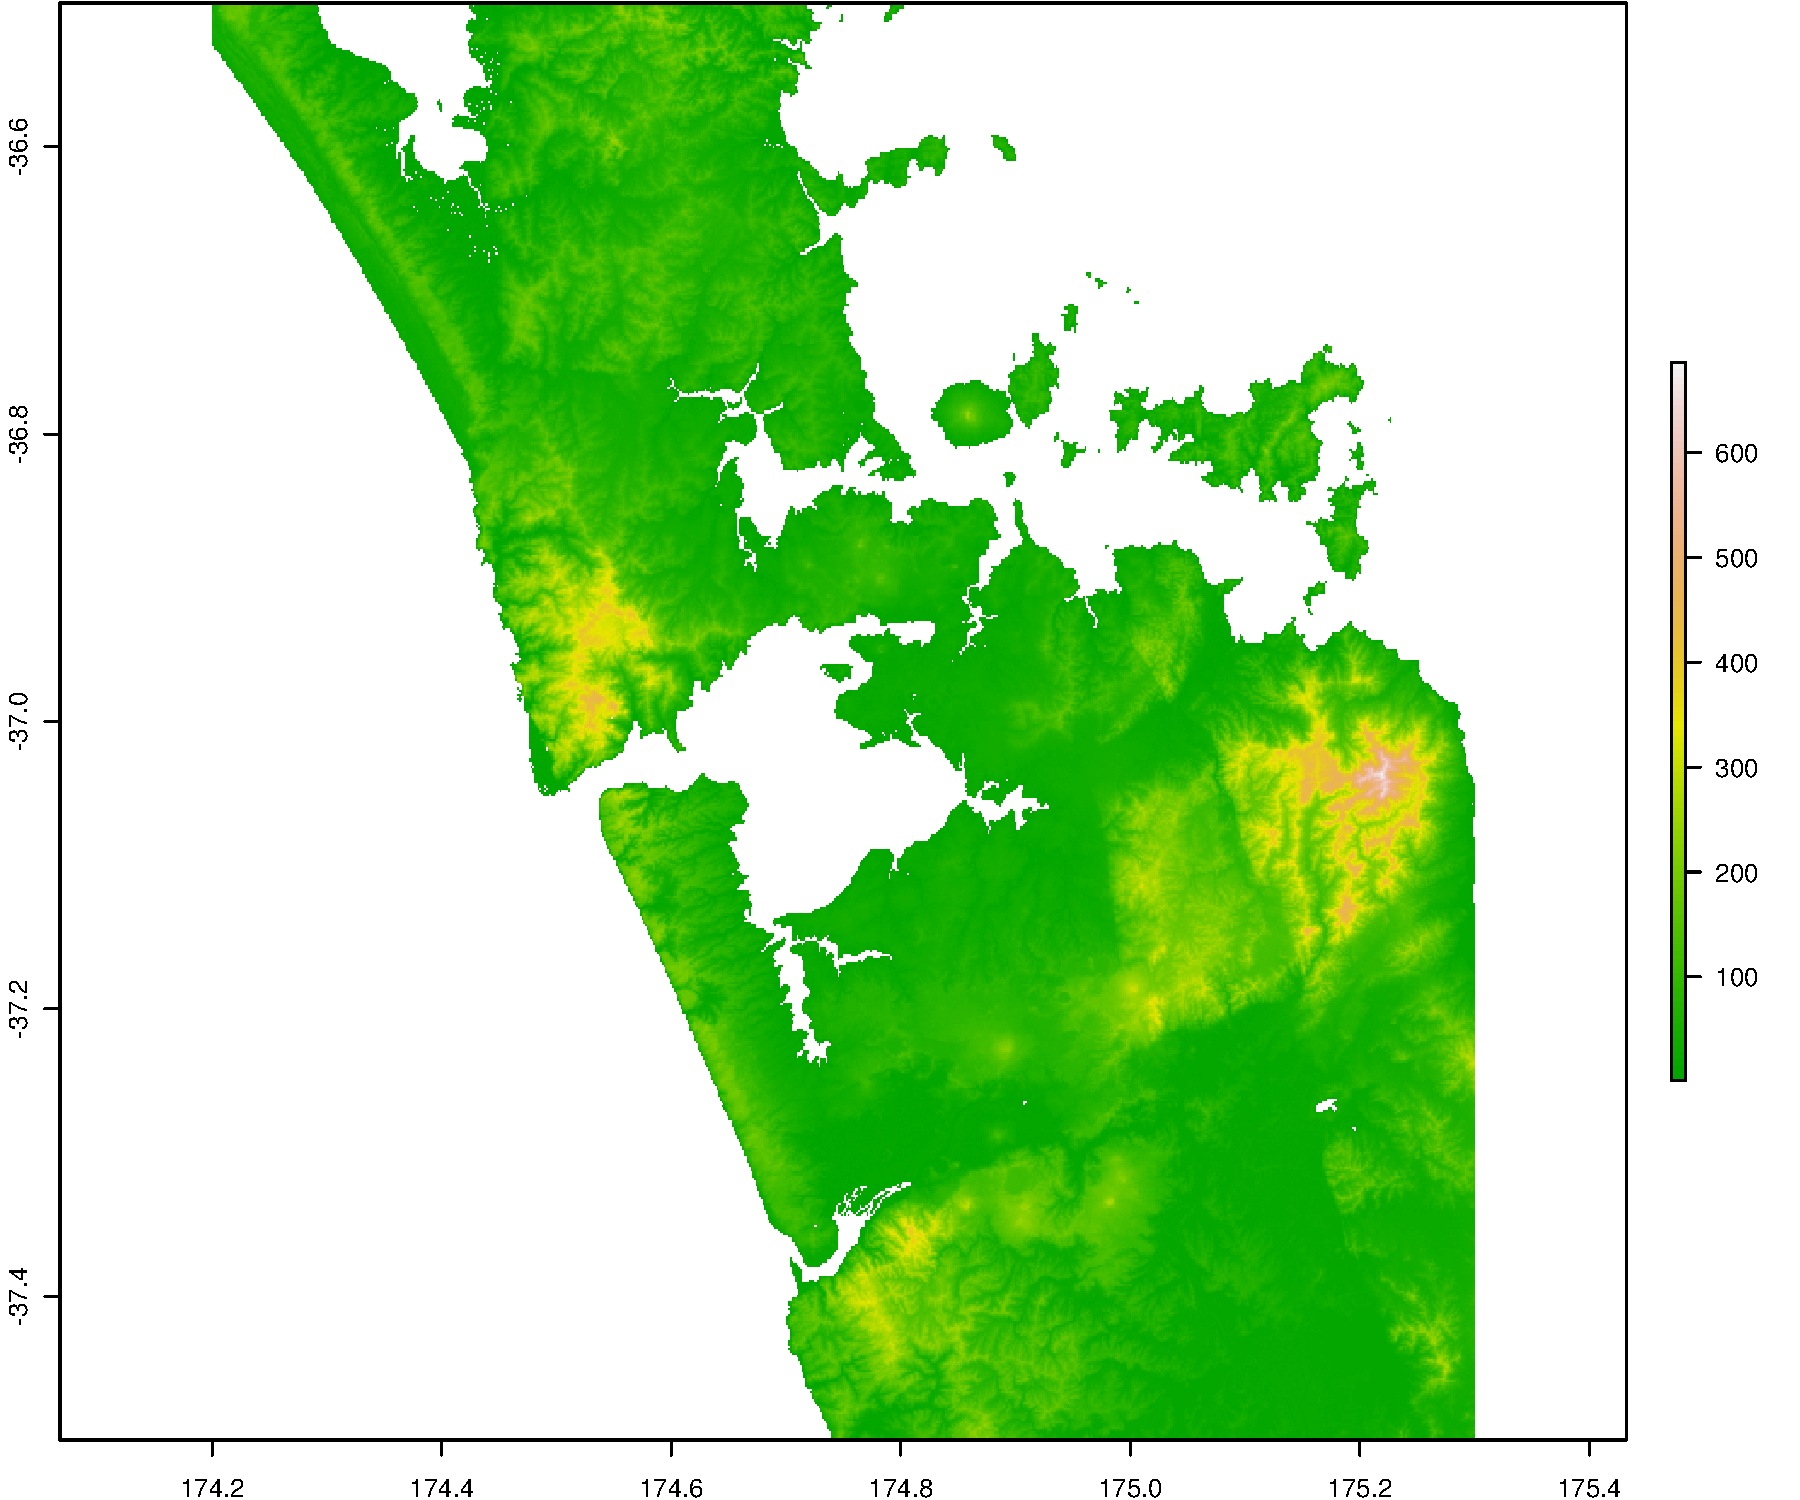
\includegraphics[width=0.65\columnwidth]{spatial_raster_example2.pdf}
% \end{figure}
% \end{onlyenv}
% \end{overlayarea}
% \end{frame}

% \begin{frame}[t,fragile]{\subsecname}{\subsubsecname}
% \begin{itemize}
% \item<1-> sp包和raster包的栅格数据类可以互相转换,例如RasterLayer对象可以强制转换为SpatialGridDataFrame对象,
% 反之亦可
% \end{itemize}

% \begin{rcode}
% > # RasterLayer对象转换为SpatialGridDataFrame对象
% > r1 <- as(out, "SpatialGridDataFrame")
% > str(r1, max.level=2)
% Formal class 'SpatialGridDataFrame' [package "sp"] with 4 slots
%   ..@ data       :'data.frame': 1584000 obs. of  1 variable:
%   ..@ grid       :Formal class 'GridTopology' [package "sp"] with 3 slots
%   ..@ bbox       : num [1:2, 1:2] 174.2 -37.5 175.3 -36.5
%   .. ..- attr(*, "dimnames")=List of 2
%   ..@ proj4string:Formal class 'CRS' [package "sp"] with 1 slot

% > # SpatialGridDataFrame转换为RasterLayer对象
% > r2 <- as(r1, "RasterLayer")
% > str(r2, max.level=2)
% Formal class 'RasterLayer' [package "raster"] with 12 slots
%   ..@ file    :Formal class '.RasterFile' [package "raster"] with 13 slots
%   ..@ data    :Formal class '.SingleLayerData' [package "raster"] with 13 slots
%   ..@ legend  :Formal class '.RasterLegend' [package "raster"] with 5 slots
%   ..@ title   : chr(0) 
%   ..@ extent  :Formal class 'Extent' [package "raster"] with 4 slots
%   ..@ rotated : logi FALSE
%   ..@ rotation:Formal class '.Rotation' [package "raster"] with 2 slots
%   ..@ ncols   : int 1320
%   ..@ nrows   : int 1200
%   ..@ crs     :Formal class 'CRS' [package "sp"] with 1 slot
%   ..@ history : list()
%   ..@ z       : list()
% \end{rcode}
% \end{frame}

% \subsection{空间数据交换}
% \subsubsection{开源GIS生态圈}

% \begin{frame}[t]{\subsecname}{\subsubsecname}
% \begin{itemize}
% %\item<1-> R属于开源生态圈,因此外部GIS文件和sp对象的交换也主要\emphText{采用开源GIS的解决方案}
% \item<1-> 除了商业的GIS软件产品(如 ArcGIS、SuperMap等)之外,世界上还有一些由\emphText{非营利性组织负责维护和管理大量的开源GIS项目},其中最著名的是由\href{https://www.osgeo.org/}{\uline{地理空间开源基金会}}(OSGeo,\emphText{O}pen \emphText{S}ource \emphText{Geo}spatial Foundation)维护的项目
% \item<1-> OSGeo维护的项目都遵循其制定的X/MIT开源许可协议,是许多GIS软件的基础,推动了开源GIS生态圈的
% 良性发展
% \end{itemize}

% \begin{overlayarea}{\textwidth}{\textheight}
% \only<2>{
% \begin{figure}[ht] \vspace{-5pt}
%   \centering
%   
\includegraphics[width=0.3\columnwidth]{osgeo-logo.png}\\
%   
\includegraphics[width=0.8\columnwidth]{foss4g.png}
%   \caption{OSGeo及其从2006年开始主办的开源GIS年度会议—FOSS4G(\emphText{F}ree and \emphText{O}pen \emphText{S}ource \emphText{S}oftware \emphText{for} \emphText{G}eoinformatics)}
% \end{figure}}

% \only<3>{
% \begin{figure}[ht] 
%   \centering
%   
\includegraphics[width=\columnwidth]{osgeo_contributors2.jpg}
%   \caption{开源GIS的贡献者们}
% \end{figure}}

% \only<4>{
% \begin{figure}[ht]
%   \centering
%   
\includegraphics[width=0.85\columnwidth]{open_source_GIS.png}
%    \caption{开源GIS生态圈} 
% \end{figure}}

% \only<5>{
%   \begin{table} \centering \small
%     \renewcommand\arraystretch{0.8} 
%     \begin{tabular}{|>{\centering\arraybackslash} m{0.2\columnwidth} |>{\centering\arraybackslash} m{0.3\columnwidth} |>{\centering\arraybackslash} m{0.35\columnwidth}|}
%       \toprule
%       \rowcolor{LightCyan}
%       \multicolumn{1}{|c|}{\textbf{GIS技术线}} & \multicolumn{1}{c|}{\textbf{商业产品}} & \multicolumn{1}{c|}{\textbf{开源解决方案}}\\\hline
%       桌面GIS & ArcMap & QGIS、GRASS GIS \\\hline
%       webGIS & ArcGIS Server & Geoserver\\\hline
%       空间数据库 & ArcSDE、Oracle Spatial & PostGIS \\\hline
%       地图服务 &  Google Maps & OpenStreetMap\\\hline
%       程序开发库 & ArcEngine & GDAL、GeoTools、proj.4\\\hline
%       元数据管理 & ArcCatalog & GeoNetwork\\
%       \bottomrule
%     \end{tabular}
%     \caption{商业和开源GIS解决方案对比}
%   \end{table}}
% \end{overlayarea}
% \end{frame}

% \subsubsection{rgdal包}

% \begin{frame}[t]{\subsecname}{\subsubsecname}
% \begin{itemize}
% \item<1-> \href{http://www.gdal.org/}{\uline{GDAL}}(Geospatial Data Abstraction Library)是Frank Warmerdam从1998年开发的空间数据转换库,从1.3.2版本开始移交给OSGeo维护,
% 成为在X/MIT许可协议下的开源库
% \item<2-> GDAL是\emphText{GIS领域最重要的底层库之一},它利用抽象数据模型来表达所支持的各种文件格式,
% 并提供一系列命令行工具来进行数据转换和处理,目前支持多达\emphText{154种栅格数据格式和93种矢量数据格式}
% \end{itemize}
% \vspace{-10pt}
% \begin{figure}\centering
%   \captionsetup[subfigure]{labelformat=empty} 
%   \subfloat[Frank Warmerdam]
%   {
\includegraphics[width=0.35\columnwidth]{frank_warmerdam.png}} \hspace{15pt}
%   \subfloat[GDAL logo]
%   {
\includegraphics[width=0.35\columnwidth]{gdal-logo.png}} 
% \end{figure}
% \end{frame}

% \begin{frame}[t,fragile]{\subsecname}{\subsubsecname}
% \begin{itemize}
% \item<1-> 许多著名的开源和商业的GIS软件都
% \emphText{在底层数据转换模块中使用GDAL库},包括ESRI ArcGIS、Google Earth、GRASS GIS等;而R本身属于开源生态圈,因此自然也选择采用
% \emphText{GDAL库作为外部GIS数据和内部sp对象相互转换的底层库}
% \item<2-> 由于原生GDAL库是ANSI C和C++开发的,所以Roger Bivand等人开发了
% \emphText{rgdal包}用于封装了GDAL库,从而可以在R中调用GDAL库函数
% \item<3-> rgdal包只是实现了在R中调用GDAL库中的C或C++函数,本质上还是要依赖GDAL,
% 因此\emphText{在载入rgdal包之前要先安装好原生的GDAL库}
% \end{itemize}

% \begin{onlyenv}<3>
% \begin{rcode}
% # rgdal包不但依赖sp包,而且依赖外部的GDAL库和proj.4库,在使用rgdal包前要确保这两个库正确安装!
% > library(rgdal)
% |\colorbox{green}{Loading required package: sp}|
% rgdal: version: 1.2-18, (SVN revision 718)
%  Geospatial Data Abstraction Library extensions to R successfully loaded
%  |\colorbox{green}{Loaded GDAL runtime}|: GDAL 2.1.3, released 2017/20/01
%  Path to GDAL shared files: /usr/share/gdal/2.1
%  GDAL binary built with GEOS: TRUE 
%  |\colorbox{green}{Loaded PROJ.4 runtime}|: Rel. 4.9.2, 08 September 2015, [PJ_VERSION: 492]
%  Path to PROJ.4 shared files: (autodetected)
%  Linking to sp version: 1.2-7 
% \end{rcode}
% \end{onlyenv}
% \end{frame}


% \subsubsection{坐标参考系统}

% \begin{frame}[t]{\subsecname}{\subsubsecname}
% \begin{itemize}
% \item<1->坐标参考系统(CRS)是测量学和制图学的核心理论,其目标是解决\emphText{“如何在平面中表示一个不规则椭球”}
% 的问题,这也是GIS系统和其他计算机系统最大的区别之一
% \item<2-> CRS的一种定义是\emphText{地理坐标系统}(GCS),用三维椭球模型来定义地球表面位置,
% 以经纬度为坐标对地球表面进行数学描述
% \end{itemize}

% \begin{overlayarea}{\textwidth}{\textheight}
% \only<2>{
% \begin{figure}[ht]
%   \centering
%   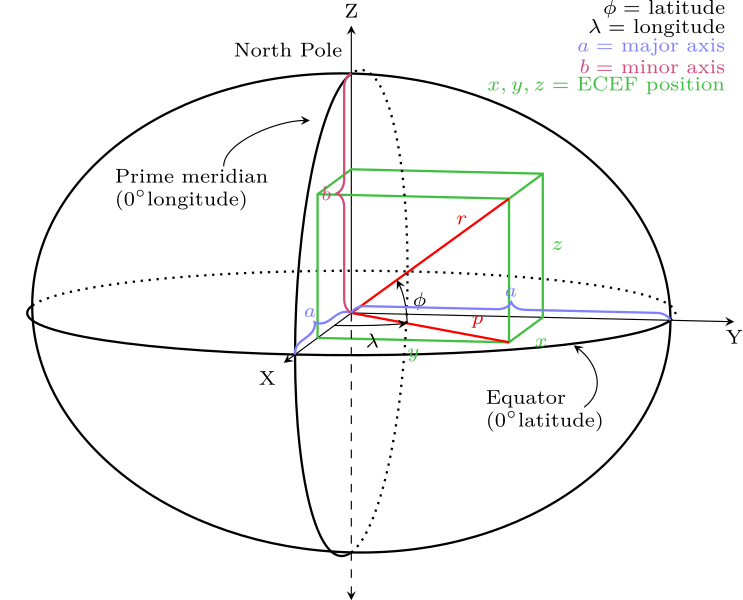
\includegraphics[width=0.55\columnwidth]{GCS.png}
%   \caption{地理坐标系统包括参考椭球体、本初子午线和经纬度单位三个要素}
% \end{figure}}
% \end{overlayarea}
% \end{frame}

% \begin{frame}[t]{\subsecname}{\subsubsecname}
% \begin{itemize}
% \item<1-> CRS的另一种定义是\emphText{投影坐标系统}(PCS),将地球表面按照某种投影类型投射到一个二维平面,以笛卡尔坐标系对地球表面进行数学描述
% \item<2-> \emphText{所有投影坐标系统都只能是对地球表面的近似描述},可以保证在某些测度(角度、距离、面积等)上是准确的,但是必然会牺牲其他方面的测度
% \end{itemize}

% \begin{overlayarea}{\textwidth}{\textheight}
% \only<1>{
% \begin{figure}[ht]
%   \centering
%   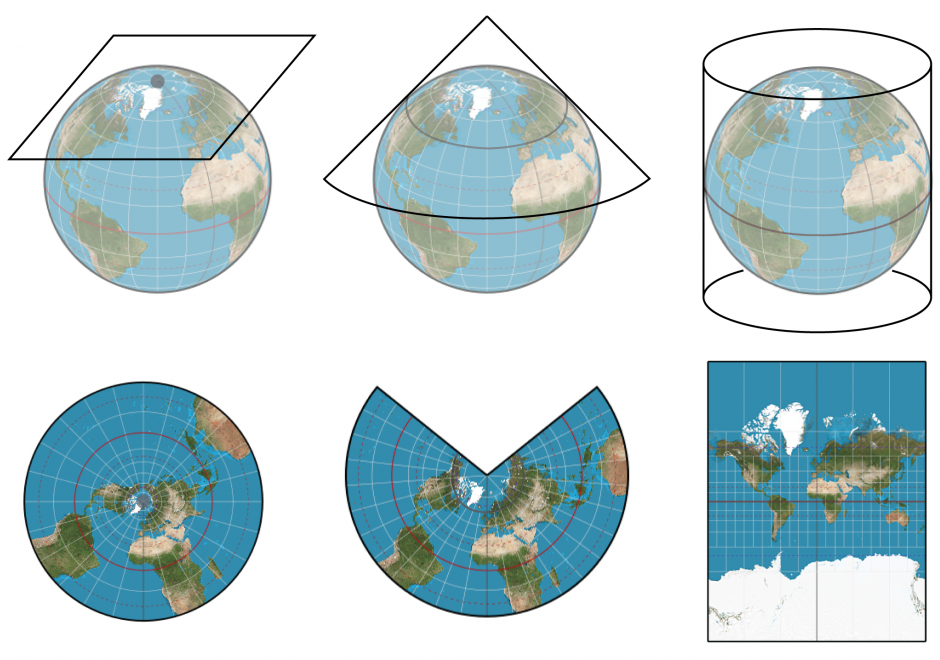
\includegraphics[width=0.55\columnwidth]{PCS.png}
%   \caption{投影坐标系统,常见的投影类型包括方位(左)、圆锥(中)和圆柱(右)}
% \end{figure}}

% \only<3>{
% \begin{figure}[ht] \vspace{-10pt}
%   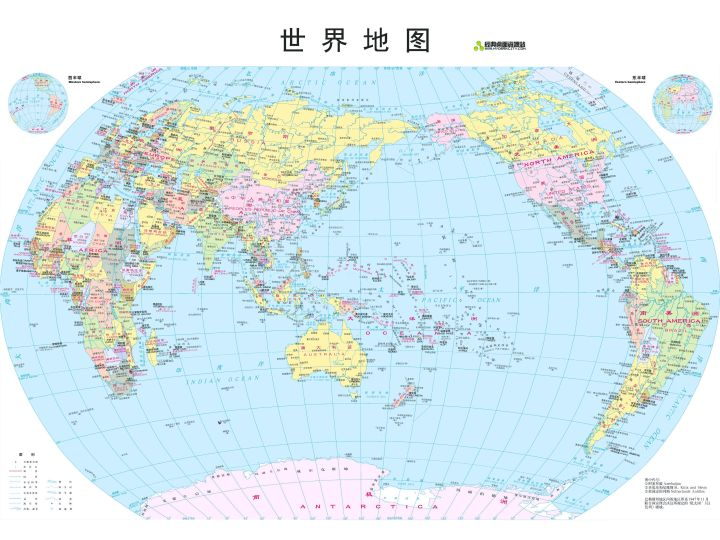
\includegraphics[width=0.55\columnwidth]{等角投影.jpg}
%   \caption{等角投影的世界地图,保证角度测度是准确的,但是面积变形严重}
% \end{figure}}

% \only<4>{
% \begin{figure}[ht]
%   \centering
%   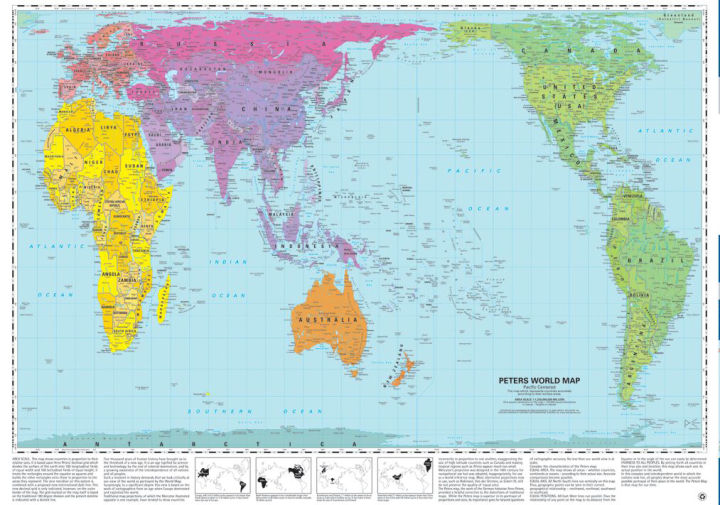
\includegraphics[width=0.55\columnwidth]{等面积投影.jpg}
%   \caption{等面积投影的世界地图,保证面积测度是准确的,但是角度变形严重}
% \end{figure}}
% \end{overlayarea}
% \end{frame}

% \begin{frame}[t,fragile]{\subsecname}{\subsubsecname}
% \begin{itemize}
% \item<1-> GDAL包底层CRS采用的是\href{http://proj4.org/}{\uline{proj.4库}},
% 因此在安装GDAL和rgdal之前要先安装proj.4
% \item<2-> proj.4是一个历史悠久的CRS库,最早是由\emphText{Gerald Evenden}开发维护,第一个版本是80年代初期用Fortran语言开发的,1985年发布了Unix系统下的C语言版本,1990发布的
% 第三个版本被命名为\emphText{proj.3},1995年发布的4.3版是Evenden开发的最后一个版本,命名为\emphText{proj.4};从2000年开始,Frank Warmerdam接管了项目的维护工作直到2008年被OSGeo接纳,
% \emphText{成为OSGeo基础开发库并由其负责维护};2018年3月proj的第5个版本发布,目前支持的地图投影已经超过\emphText{138个}
% \end{itemize}

% \begin{onlyenv}<3>
% \begin{rcode}
% # rgdal包载入前要先做proj.4库依赖性检查
% > library(rgdal)
% Loading required package: sp
% rgdal: version: 1.2-18, (SVN revision 718)
%  Geospatial Data Abstraction Library extensions to R successfully loaded
%  Loaded GDAL runtime: GDAL 2.1.3, released 2017/20/01
%  Path to GDAL shared files: /usr/share/gdal/2.1
%  GDAL binary built with GEOS: TRUE 
%  |\colorbox{green}{Loaded PROJ.4 runtime}|: Rel. 4.9.2, 08 September 2015, [PJ_VERSION: 492]
%  Path to PROJ.4 shared files: (autodetected)
%  Linking to sp version: 1.2-7 
% \end{rcode}
% \end{onlyenv}
% \end{frame}

% \begin{frame}[t,fragile]{\subsecname}{\subsubsecname}
% \begin{itemize}
% \item<1-> proj.4库有一套CRS定义的规范,表示方法是CRS中的“参数标签=值”(不能有空格),每个参数标签以“+”开始并且用空格
% 区分不同的标签/值对,\emphText{最终形成一个字符串}
% \end{itemize}

% \begin{overlayarea}{\textwidth}{\textheight}
% \only<1>{ 
%   \begin{table} \centering \small
%     \renewcommand\arraystretch{0.7} 
%     \begin{tabular}{|>{\centering\arraybackslash} m{0.2\columnwidth} |>{\centering\arraybackslash} m{0.65\columnwidth} |}
%       \toprule
%       \rowcolor{LightCyan}
%       \multicolumn{1}{|c|}{\textbf{参数标签}} & \multicolumn{1}{c|}{\textbf{含义}} \\\hline
%       proj & 投影名称,定义PCS;当=longlat时定义GCS \\\hline
%       ellps & 椭球体名称\\\hline
%       datum & 基准面名称\\\hline
%       pm & 备用本初子午线(通常是一个城市名称) \\\hline
%       lon\_0,lat\_0 & 中央经线和纬度原点\\\hline
%       towgs84 & 三参数或七参数基准面转换\\\hline
%       x\_0,y\_0 & 东伪偏移和北伪偏移\\\hline
%       k\_0 & 比例因子\\\hline
%       a,b & 椭球体长短轴长度\\\hline
%       axis & 轴方向\\\hline
%       zone & UTM时区\\\hline
%       init & CRS定义文件存放路径和关键字\\\hline
%       no\_defs & 不使用默认的定义文件\\
%       \bottomrule
%     \end{tabular}
%     \caption{proj.4主要的参数标签}
%   \end{table}}

% \begin{onlyenv}<2>
% \begin{rcode}
% # 定义深圳西安1980坐标系3度带投影:投影名称横轴墨卡托,中央经线东经114度,比例因子1,东伪偏移500000,椭球体长轴
% 长度6378140米,短轴长度6356755.288157528米,单位米
% > CRS("+proj=tmerc +lat_0=0 +lon_0=114 +k=1 +x_0=500000 +y_0=0 +a=6378140 +b=6356755.288157528 +units=m +no_defs") 
% CRS arguments:
%  +proj=tmerc +lat_0=0 +lon_0=114 +k=1 +x_0=500000 +y_0=0 +a=6378140 +b=6356755.288157528 +units=m +no_defs 

% # 定义深圳北京1954坐标系3度带投影:投影名称横轴墨卡托,中央经线东经114度,比例因子1,东伪偏移500000,
% 椭球体为苏联克拉索夫斯基椭球体,单位米
% > CRS("+proj=tmerc +lat_0=0 +lon_0=114 +k=1 +x_0=500000 +y_0=0 +ellps=krass +units=m +no_defs") 
% CRS arguments:
%  +proj=tmerc +lat_0=0 +lon_0=114 +k=1 +x_0=500000 +y_0=0 +ellps=krass +units=m +no_defs 

% # 定义北京1954GCS:椭球体为苏联克拉索夫斯基
% > CRS("+proj=longlat +ellps=krass +no_defs")
% CRS arguments: +proj=longlat +ellps=krass +no_defs 

% # 定义美国田纳西州PCS:投影名称兰勃特等角圆锥投影,椭球体是Clarke 1866椭球,基准面为北美1927基准面
% > CRS("+proj=lcc +lat_1=35.25 +lat_2=36.41666666666666 +lat_0=34.66666666666666 +lon_0=-86 +x_0=609601.2192024384 +y_0=30480.06096012192 +datum=NAD27 +units=us-ft +no_defs")
% CRS arguments:
%  +proj=lcc +lat_1=35.25 +lat_2=36.41666666666666 +lat_0=34.66666666666666 +lon_0=-86 +x_0=609601.2192024384 +y_0=30480.06096012192 +datum=NAD27 +units=us-ft +no_defs +ellps=clrk66 +nadgrids=@conus,@alaska,@ntv2_0.gsb,@ntv1_can.dat 
% \end{rcode}
% \end{onlyenv}
% \end{overlayarea}
% \end{frame}

% \begin{frame}[t,fragile]{\subsecname}{\subsubsecname}
% \begin{itemize}
% \item<1-> 欧洲石油调查组(\emphText{EPSG},European Petroleum Survey Group)为了能够更好地调查世界石油储量,从1986年开始收集各地区CRS参数,
% 并且给每个CRS进行统一编号管理,最终形成并发布\href{http://www.epsg.org/}{\uline{EPSG标准数据集}}
% \item<1-> 目前EPSG数据集已经成为世界标准CRS数据集之一,proj.4库可以用
% \emphText{init标签参数}调用指定编号的CRS参数
% \end{itemize}

% \begin{onlyenv}<2>
% \begin{rcode}
% # WGS84 GCS的编号是4326
% > CRS("+init=epsg:4326")
% CRS arguments:
%  +init=epsg:4326 +proj=longlat +datum=WGS84 +no_defs +ellps=WGS84 +towgs84=0,0,0 

% # 3857是一个重要的编号,因为各大互联网地图都以它为基准,例如Google Maps,Bing Maps、OpenStreetMap等
% > CRS("+init=epsg:3857")
% CRS arguments:
%  +init=epsg:3857 +proj=merc +a=6378137 +b=6378137 +lat_ts=0.0 +lon_0=0.0 +x_0=0.0 +y_0=0 +k=1.0 +units=m +nadgrids=@null +no_defs

% # 北京1954 GCS的编号是4214
% > CRS("+init=epsg:4214")
% CRS arguments:
%  +init=epsg:4214 +proj=longlat +ellps=krass +towgs84=15.8,-154.4,-82.3,0,0,0,0 +no_defs

% # 北京1954在深圳的三度分带PCS编号是2435
% > CRS("+init=epsg:2435")
% CRS arguments:
%  +init=epsg:2435 +proj=tmerc +lat_0=0 +lon_0=114 +k=1 +x_0=500000 +y_0=0 +ellps=krass +towgs84=15.8,-154.4,-82.3,0,0,0,0 +units=m +no_defs 
% \end{rcode}
% \end{onlyenv}
% \end{frame}

% \begin{frame}[t,fragile]{\subsecname}{\subsubsecname}
% \begin{itemize}
% \item<1-> 由于各地区CRS都不尽相同,因此为了坐标能在统一CRS中表达,
% 坐标转换成为空间数据处理的常规操作,通常包括\emphText{GCS和PCS互转(投影与反投影)}、\emphText{基准面互转}
% 和\emphText{PCS互转}
% \item<2-> proj.4库中提供了\emphText{cs2cs}函数用于坐标的CRS转换,rgdal包中也提供了类似的
% \emphText{spTransform函数},可以将一个sp对象定义的CRS转换到另一个CRS
% \end{itemize}

% \begin{overlayarea}{\textwidth}{\textheight}
% \begin{onlyenv}<3>
% \begin{rcode}
% # 定义GCS坐标的x和y位置
% > y <- as.numeric(char2dms("43d38'33.24\"N"))
% > x <- as.numeric(char2dms("79d23'13.7\"W"))
% # 将坐标转换为空间点对象,并定义CRS为基准面wgs84的GCS
% > xy <- SpatialPoints(cbind(x,y),proj4string=CRS("+proj=longlat +datum=WGS84"))
% > xy@coords
%              x        y
% [1,] -79.38714 43.64257
% > spTransform(xy,CRS("+proj=utm +zone=17 +datum=WGS84"))@coords
%             x       y
% [1,] 630084.3 4833439
% \end{rcode}
% \end{onlyenv}

% \begin{onlyenv}<4>
% \begin{rcode}
% # 读取中国地图边界
% > library(maps)
% > library(maptools)
% > china<- map("world", "china", fill=TRUE,plot=FALSE)
% > tw <- map("world","taiwan",fill=TRUE,plot=FALSE)
% > china$x <- c(china$x,NA,tw$x)
% > china$y <- c(china$y,NA,tw$y)
% > china$range <- c(range(china$range[1:2],tw$range[1:2]),range(china$range[3:4],tw$range[3:4]))
% > china$names <- c(china$names,tw$names)
% # 定义GCS为WGS84,并创建空间面对象
% > p4s <- CRS("+proj=longlat +datum=WGS84")
% > SPchina <- map2SpatialPolygons(china,IDs=sapply(china$names, function(x) x[1]),proj4string=p4s)
% # 将WGS84坐标投影到UTM投影坐标系统
% > SPchina2 <-spTransform(SPchina,CRS("+proj=utm +zone=49 +datum=WGS84"))
% \end{rcode}
% \end{onlyenv}

% \only<5>{ \vspace{-15pt}
% \begin{figure}[ht]
%   \centering
%   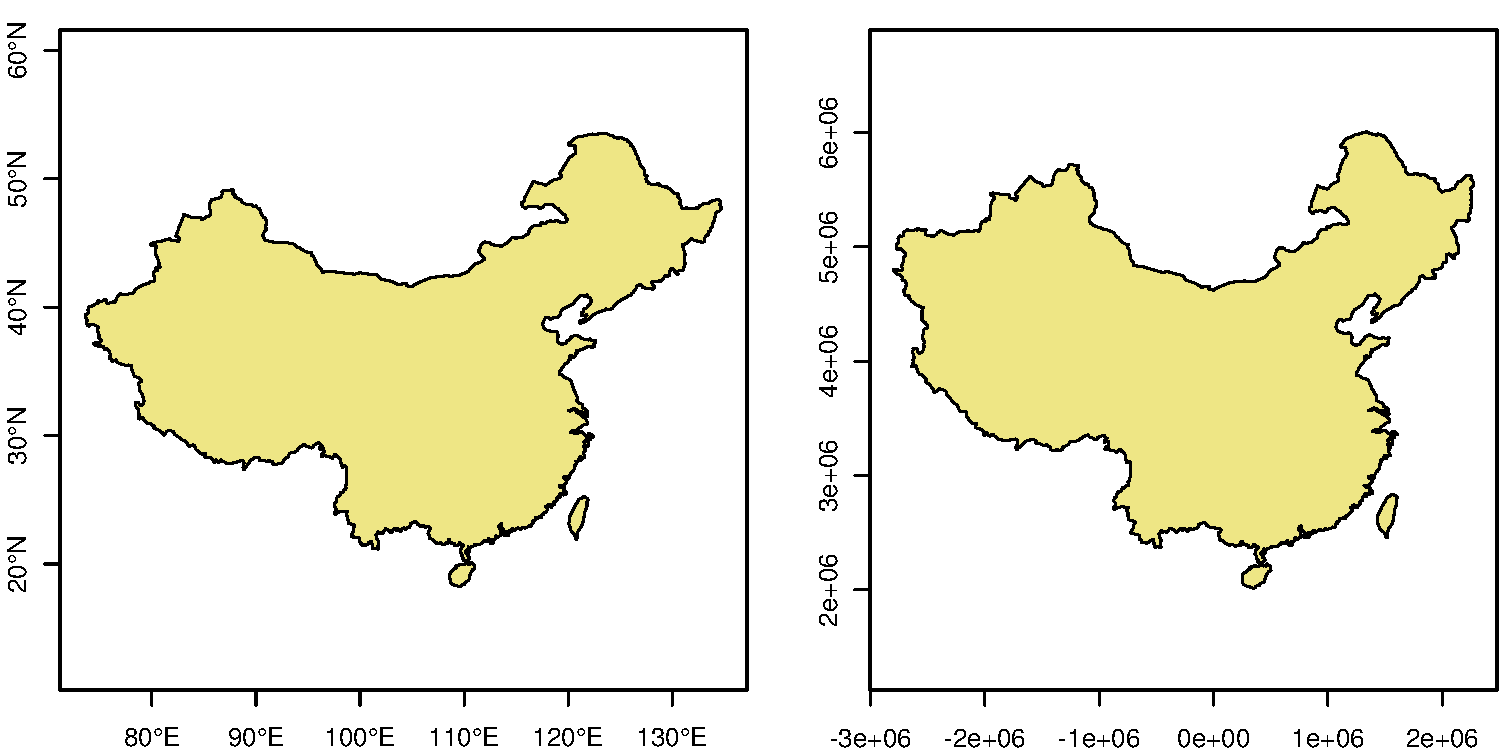
\includegraphics[width=0.8\columnwidth]{spTransform_example.pdf}
%   \caption{中国地图的坐标转换:左图为WGS84地理坐标系,右图是UTM投影坐标系}
% \end{figure}}
% \end{overlayarea}
% \end{frame}

% \subsubsection{矢量格式文件交换}
% \begin{frame}[t,fragile]{\subsecname}{\subsubsecname}
% \begin{itemize} 
% \item<1-> GDAL库最初不支持矢量数据,因此引入了参考OGC开源简单要素规范设计的\emphText{OGR库},
% 实现了外部矢量数据交换功能
% \item<2-> OGR全称是\emphText{OGR简单要素库}(OGR Simple Feature Library),是用C++编写的开源矢量数据格式交换库,
% 其架构是建立统一的简单要素抽象模型,并在此基础\emphText{通过外部驱动程序扩展各种数据交换的功能},
% 这对于复杂多样的矢量数据交换具有极大的灵活性
% \item<3-> 从设计上\emphText{OGR库和sp包都是采用简单要素规范对矢量数据建模},因此外部数据可以
% 通过rgdal包调用OGR库函数来读取,并转换为sp对象;同样sp对象也可以通过逆操作写入外部文件,
% 从而实现在R体系中的矢量数据格式交换
% \end{itemize}
% \end{frame}

% \begin{frame}[t,fragile]{\subsecname}{\subsubsecname}
% \begin{itemize} 
% \item<1-> rgdal包中提供了\emphText{readOGR}函数和\emphText{writeOGR}函数分别实现OGR库读取的外部数据
% 转换sp对象以及sp对象导出到外部文件
% \item<2-> readOGR函数至少需要两个参数:\emphText{dsn参数用于指定外部数据源的位置},\emphText{layer参数用于指定要素图层名称};例如,对于shapefile格式文件,dsn是文件存放的目录,layer是文件名
% \item<3-> writeOGR除了dsn和layer两个必需参数之外,还至少需要一个参数用于\emphText{指定要导出的sp对象},
% 以及一个参数\emphText{用于指定外部驱动程序}
% \end{itemize}

% \begin{overlayarea}{\textwidth}{\textheight}
% \begin{onlyenv}<1>
% \begin{rcode}
% # 用ogrInfo函数获取shapefile格式文件scot的信息
% > ogrInfo("./data","scot")
% Source: "/home/mono/Documents/tex_projects/r_guide_slide/data", layer: "scot"
% Driver: ESRI Shapefile; number of rows: 56 
% Feature type: wkbPolygon with 2 dimensions
% Extent: (-8.621389 54.62722) - (-0.7530556 60.84444)
% LDID: 0 
% Number of fields: 2 
%   name type length  typeName
% 1 NAME    4     16    String
% 2   ID   12     16 Integer64
% \end{rcode}
% \end{onlyenv}

% \begin{onlyenv}<2>
% \begin{rcode}
% # 用readOGR文件读取shapefile格式文件,该函数会根据文件格式自动调用对应驱动程序
% # 读取后的数据被转换为sp对象scot\_LL,从而进入R系统,可以继续后续的数据操作
% > scot_LL <- |\colorbox{green}{readOGR}|(dsn="data/scot.shp", layer="scot", integer64="allow.loss")
% OGR data source with driver: ESRI Shapefile 
% Source: "/home/mono/Documents/tex_projects/r_guide_slide/data/scot.shp", layer: "scot"
% with 56 features
% It has 2 fields
% Integer64 fields read as signed 32-bit integers:  ID 
% > proj4string(scot_LL) # 原始shapefile文件缺失prj文件,因此CRS为NA值
% [1] NA
% > proj4string(scot_LL) <- CRS("+proj=longlat +ellps=WGS84") # 为sp对象定义CRS
% > str(scot_LL,max.level=2)
% Formal class 'SpatialPolygonsDataFrame' [package "sp"] with 5 slots
%   ..@ data       :'data.frame': 56 obs. of  2 variables:
%   ..@ polygons   :List of 56
%   ..@ plotOrder  : int [1:56] 55 51 12 49 1 50 52 3 6 53 ...
%   ..@ bbox       : num [1:2, 1:2] -8.621 54.627 -0.753 60.844
%   .. ..- attr(*, "dimnames")=List of 2
%   ..@ proj4string:Formal class 'CRS' [package "sp"] with 1 slot
% \end{rcode}
% \end{onlyenv}

% \begin{onlyenv}<3>
% \begin{rcode}
% # 定义外部驱动程序,驱动程序名称可以用ogrDrivers()函数查看
% > drv <- "ESRI Shapefile"
% # 将sp对象写出到一个外部文件scot\_LL
% > |\colorbox{green}{writeOGR}|(scot_LL, dsn = ".", layer = "scot_LL", driver = drv)
% # 由于scot\_LL包含CRS,因此导出的shapefile文件中还包括prj文件
% > list.files("./data",pattern = "^scot_LL")
% [1] "scot_LL.dbf" "scot_LL.prj" "scot_LL.shp" "scot_LL.shx"
% \end{rcode}
% \end{onlyenv}
% \end{overlayarea}
% \end{frame}

% \subsubsection{栅格格式文件交换}
% \begin{frame}[t,fragile]{\subsecname}{\subsubsecname}
% \begin{itemize} 
% \item<1-> 与矢量数据类似,GDAL也是通过调用外部驱动程序实现不同格式栅格数据的读取;而rgdal包也专门提供了
% \emphText{readGDAL}函数和\emphText{writeGDAL}函数用于外部栅格格式文件和sp对象的交换
% \item<2-> 由于栅格文件体积较大,而且可能存储在不同波段,因此除了直接读取之外,
% readGDAL和writeGDAL函数还可以用\emphText{band}、\emphText{offset}、\emphText{region.dim}、
% \emphText{output.dim}等参数\emphText{控制数据的局部读写}
% \end{itemize}

% \begin{overlayarea}{\textwidth}{\textheight}
% \begin{onlyenv}<1>
% \begin{rcode}
% > fn <- system.file("pictures/erdas_spnad83.tif", package = "rgdal")[1]
% # 读取tif格式文件,readGDAL自动调用外部驱动程序GTiff
% > x <- readGDAL(fn)
% /home/mono/Softwares/R/3.4/rgdal/pictures/erdas_spnad83.tif has GDAL driver GTiff 
% and has 658 rows and 571 columns
% # 读取的数据被转换成sp对象,从而将外部数据导入R系统
% > str(x,max.level=2)
% Formal class 'SpatialGridDataFrame' [package "sp"] with 4 slots
%   ..@ data       :'data.frame': 375718 obs. of  1 variable:
%   ..@ grid       :Formal class 'GridTopology' [package "sp"] with 3 slots
%   ..@ bbox       : num [1:2, 1:2] 78999 1412948 101839 1439268
%   .. ..- attr(*, "dimnames")=List of 2
%   ..@ proj4string:Formal class 'CRS' [package "sp"] with 1 slot
% \end{rcode}
% \end{onlyenv}

% \begin{onlyenv}<2>
% \begin{rcode}
% > y <- readGDAL(fn, offset=c(50, 100), region.dim=c(400, 400))
% /home/mono/Softwares/R/3.4/rgdal/pictures/erdas_spnad83.tif has GDAL driver GTiff 
% and has 658 rows and 571 columns
% > str(y,max.level=2)
% Formal class 'SpatialGridDataFrame' [package "sp"] with 4 slots
%   ..@ data       :'data.frame': |\colorbox{green}{160000}| obs. of  1 variable:
%   ..@ grid       :Formal class 'GridTopology' [package "sp"] with 3 slots
%   ..@ bbox       : num [1:2, 1:2] 82999 1421268 98999 1437268
%   .. ..- attr(*, "dimnames")=List of 2
%   ..@ proj4string:Formal class 'CRS' [package "sp"] with 1 slot
% \end{rcode}
% \end{onlyenv}

% \only<3>{ \vspace{-20pt}
% \begin{figure}[ht]
%   \centering
%   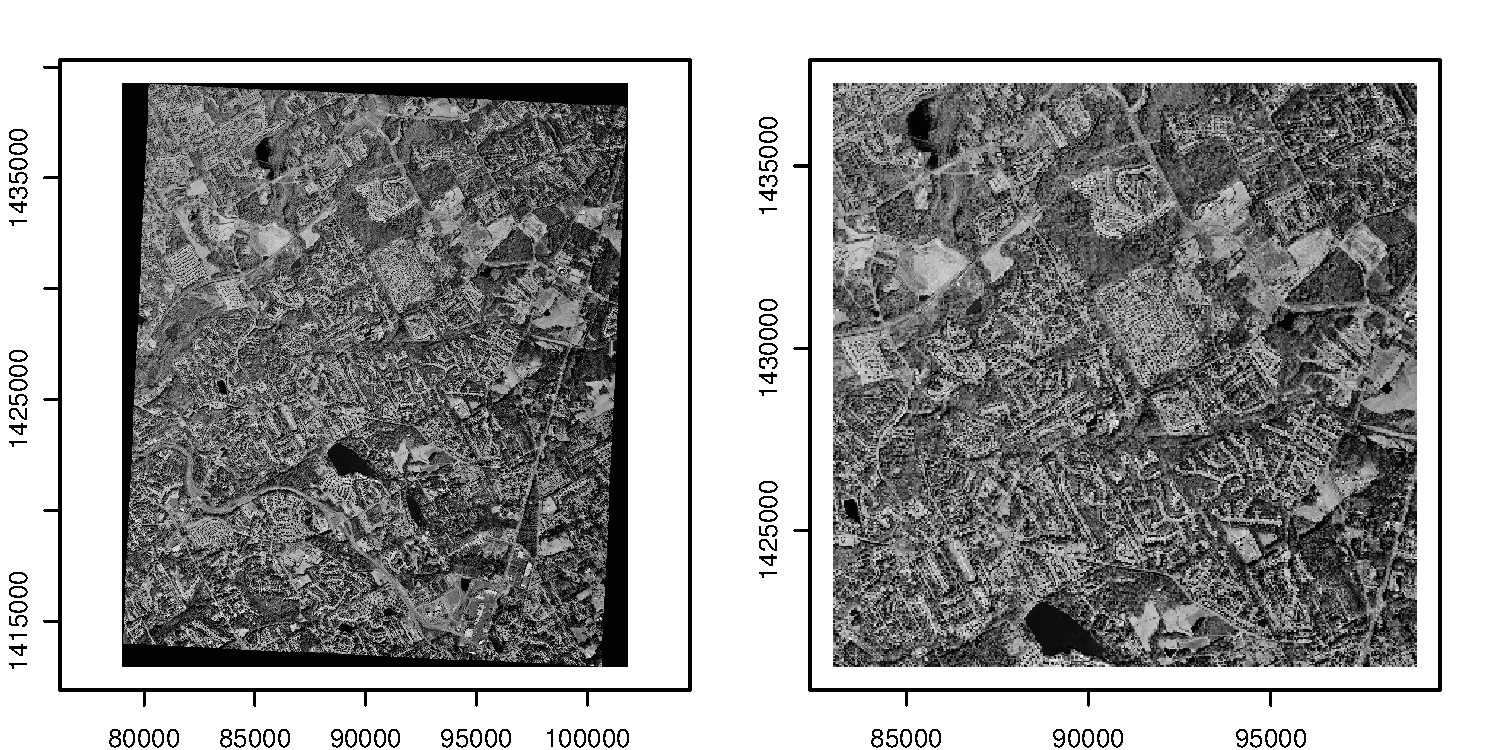
\includegraphics[width=0.85\columnwidth]{readgdal_example1.pdf}
%   \caption{读取外部栅格文件:左图是读取全部数据,右图是读取局部数据}
% \end{figure}}

% \begin{onlyenv}<4>
% \begin{rcode}
% # 读取原始tiff格式文件到sp对象
% > auck_el1 <- readGDAL("data/70042108.tif")
% data/70042108.tif has GDAL driver GTiff 
% and has 1200 rows and 1320 columns
% > is.na(auck_el1$band1) <- auck_el1$band1 <= 0 |$\mid{}$|auck_el1$band1 > 1e+4
% > # 自定义数据分类
% > brks <- c(0,10,20,50,100,150,200,300,400,500,600,700)
% > # 自定义渐变颜色方案
% > pal <- terrain.colors(11)
% > length(pal) == length(brks)-1
% [1] TRUE
% > # 将数据按照等级进行划分
% > auck_el1$band1 <- findInterval(auck_el1$band1, vec=brks, all.inside=TRUE)-1
% > # 将sp对象导出到外部栅格文件,其中栅格要素按照自定义等级配色
% > writeGDAL(auck_el1, "data/demIndex.tif", drivername="GTiff", type="Byte", colorTable=list(pal), mvFlag=length(brks)-1)
% \end{rcode}
% \end{onlyenv}

% \begin{onlyenv}<5>
% \vspace{-10pt}
% \begin{columns} 
%         \begin{column}{.38\textwidth}
%           \begin{figure}
%             \centering
%             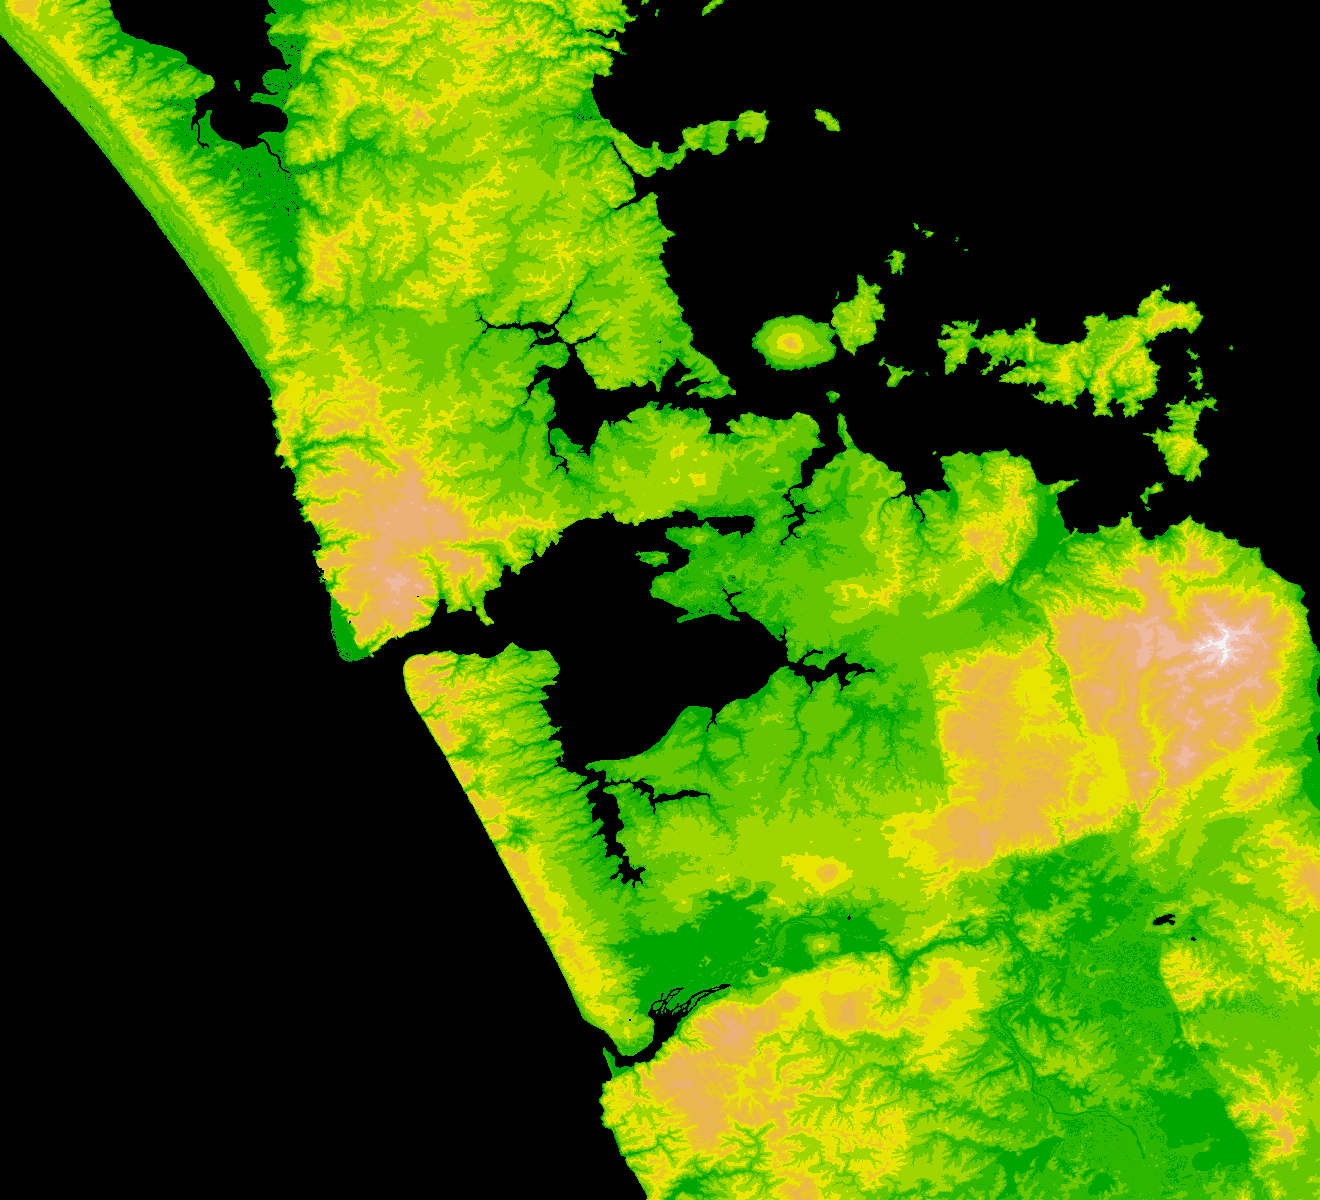
\includegraphics[width=\columnwidth]{demIndex.png}
%           \end{figure}
%         \end{column}

%         \begin{column}{.65\textwidth}
% \centering
% \begin{rcode}
% # GDALinfo封装了GDAL库函数gdalinfo,用于读取文件的信息
% > |\colorbox{green}{GDALinfo}|("figures/demIndex.tif")
% rows        1200 
% columns     1320 
% bands       1 
% lower left origin.x        174.2 
% lower left origin.y        -37.5 
% res.x       0.0008333333 
% res.y       0.0008333333 
% ysign       -1 
% oblique.x   0 
% oblique.y   0 
% driver      GTiff 
% projection  +proj=longlat +datum=WGS84 +no_defs 
% file        data/demIndex.tif 
% apparent band summary:
%   GDType hasNoDataValue NoDataValue blockSize1 blockSize2
% 1   Byte           TRUE          11          6       1320
% apparent band statistics:
%   Bmin Bmax Bmean Bsd
% 1    0  255    NA  NA
% Metadata:
% AREA_OR_POINT=Area 
% \end{rcode}
%         \end{column}
%       \end{columns}
% \end{onlyenv}
% \end{overlayarea}
% \end{frame}

% \begin{frame}[t,fragile]{\subsecname}{\subsubsecname}
% \begin{itemize} 
% \item<1-> readGDAL函数底层实际上是创建了一个能够被GDAL库中\emphText{GDALDriver}类对象识别的Dataset类
% \item<2-> rgdal包完整封装了GDAL库的\emphText{GDALMajorObject}抽象基类,
% 并且在S4系统下派生出只读的\emphText{GDALReadOnlyDataset}以及可读写的\emphText{GDALDataset}等具体实现类
% \end{itemize}

% \begin{overlayarea}{\textwidth}{\textheight}
% \only<3>{
% \begin{figure}[ht]
%   \centering
%   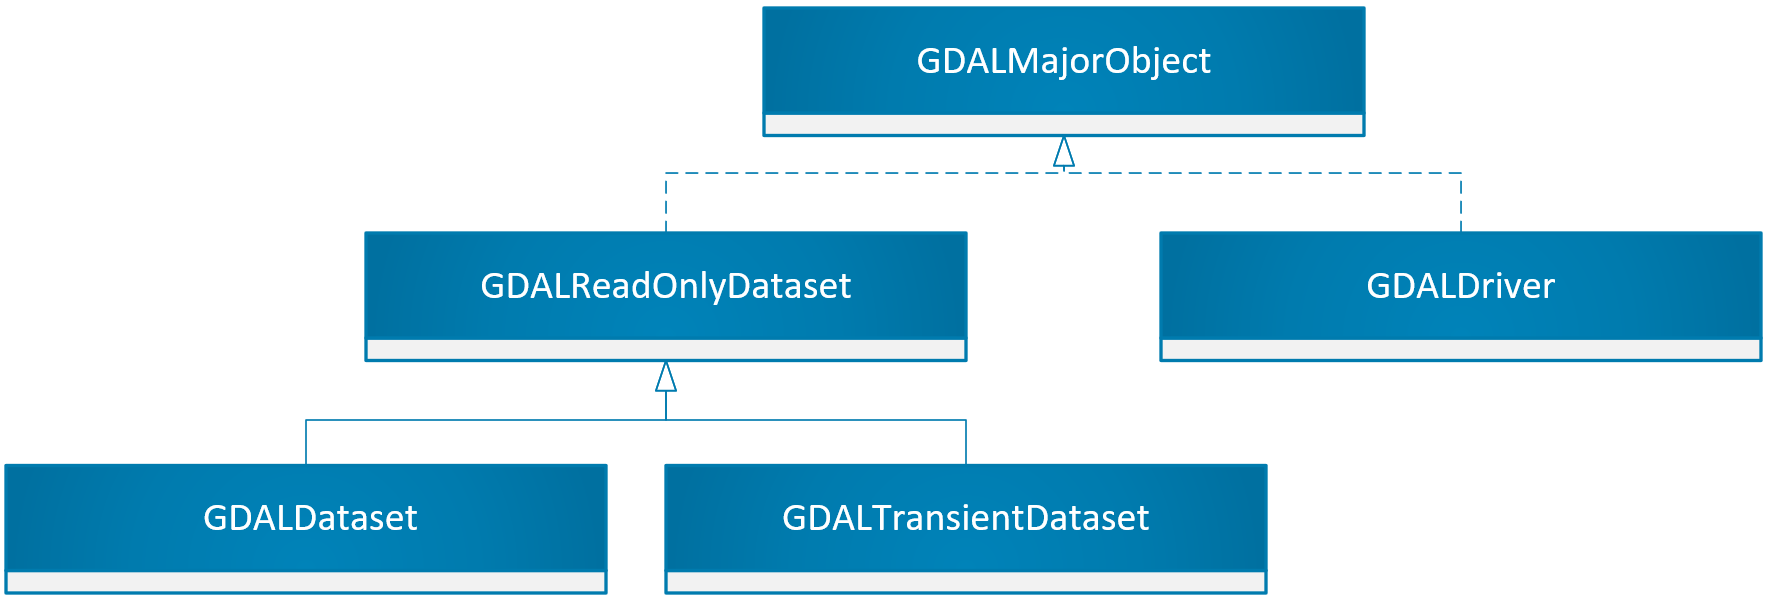
\includegraphics[width=\columnwidth]{rgdal_class.png}
%   \caption{rgdal包的栅格数据类结构图}
% \end{figure}}
% \end{overlayarea}
% \end{frame}

% \begin{frame}[t,fragile]{\subsecname}{\subsubsecname}
% \begin{itemize} 
% \item<1-> \sloppy rgdal包提供\emphText{GDAL.open}函数用于打开外部数据,
% 这个函数不会直接读取数据到内存,而是通过底层GDAL对象\emphText{GDALReadOnlyDataset}存储文件句柄
% \item<1-> 当需要数据时调用\emphText{asSGDF\_GROD}函数,该函数会根据句柄和数据大小分配内存空间,
% 并转换为R中能够识别的sp对象;另外,在文件使用完后必须要调用\emphText{GDAL.close}函数,
% 用来释放内存空间并销毁文件句柄
% \end{itemize}

% \begin{overlayarea}{\textwidth}{\textheight}
% \begin{onlyenv}<2>
% \begin{rcode}
% fn <- system.file("pictures/erdas_spnad83.tif", package = "rgdal")[1]
% # GDAL.open函数读取文件数据到GDALReadOnlyDataset对象,而不是直接转换为sp对象,
% x <- |\colorbox{green}{GDAL.open}|(fn)
% # 这个GDAL对象存储了外部文件句柄
% > str(x)
% Formal class 'GDALReadOnlyDataset' [package "rgdal"] with 1 slot
%   ..|\colorbox{green}{@ handle:<externalptr>}|
% # rgdal包提供一系列函数根据文件句柄读取文件信息
% > dim(x)  # 栅格数据维度
% [1] 658 571
% > xx <- |\colorbox{green}{getDriver}|(x) # 转换为驱动程序类
% > |\colorbox{green}{getDriverLongName}|(xx) # 驱动程序完整名称
% [1] "GeoTIFF"
% # 将GDAL对象转换为sp对象,从而进入R系统
% > y <- |\colorbox{green}{asSGDF\_GROD}|(x,output.dim=c(400, 400)) # 这里也可以局部读取数据
% > class(y)
% [1] "SpatialGridDataFrame"
% attr(,"package")
% [1] "sp"
% # 释放GDAL对象,解除对外部文件的锁定
% > |\colorbox{green}{GDAL.close}|(x)
% \end{rcode}
% \end{onlyenv}
% \end{overlayarea}
% \end{frame}

% \subsubsection{其他空间数据交换包}
% \begin{frame}[t]{\subsecname}{\subsubsecname}
% \begin{itemize} 
% \item \emphText{maptools}:提供ESRI ArcGIS格式数据文件的读写函数;
% 相比其他包最大的优势是不依赖外部程序,\emphText{但是该包部分函数已经不再维护}
% \item \emphText{RQIS,rgrass7,RSAGA}:这些包分别是主流开源GIS软件\href{https://www.qgis.org/}{\uline{QGIS}}、\href{https://grass.osgeo.org/}{\uline{GRASS GIS}}和\href{http://www.saga-gis.org/}{\uline{SAGA}}的封装包,都是通过R内部的\emphText{system函数}把命令传至外部程序实现对接口的调用,因此具体功能实现都依赖外部程序,在使用前要先安装相应的GIS软件;由于这些软件本身具有完整的GIS功能,所以除了可以读写外部文件之外,这些包还具有丰富的GIS数据管理和分析功能
% \item \emphText{sf}:近几年CRAN发布的简单空间要素包,
% 相比sp包,sf对OGC简单要素标准的支持更完整,定义了全部17种简单要素,甚至包括三维对象和线性参考对象;sf包依赖GDAL库提供对矢量数据文件的交换功能
% \item \emphText{RgoogleMaps,OpenStreetMap,ggmap,baidumap}:这些包通过互联网地图API实现了对地图数据的调用
% \item Roger Bivand目前维护着空间数据相关包信息的整理工作,CRAN上有\href{https://cran.r-project.org/web/views/Spatial.html}{\uline{专门的文章}}会定期更新这些信息
% \end{itemize}
% \end{frame}

\subsection{基础绘图方法}
\begin{frame}[t]{\subsecname}
\begin{itemize} 
\item<1-> R的两套绘图系统都提供对基础绘图要素的绘制功能,包括点、线、面、栅格和颜色等,
而通过sp包可以将空间数据转换为这些绘图要素能够识别的底层对象,
因此\emphText{空间数据绘图要素和普通数据绘图要素并没有本质区别}
\item<2-> 在基础绘图系统graphics包和grid绘图系统lattice包基础上,sp包针对空间数据对象的特点重载了
两个包的主要绘图函数,并充分考虑了空间可视化的特点,添加了诸如指北针、比例尺等专业地图要素的绘制,\emphText{使得空间数据可视化在方法尽量与普通数据绘图一致的基础上又体现出专业性},这样用户可以把更多的精力放在处理和分析空间数据上,而不需要再专门花时间学习一套新的绘图系统\end{itemize}
\end{frame}

\subsubsection{绘制空间对象}
\begin{frame}[t,fragile]{\subsecname}{\subsubsecname}
\begin{itemize} 
\item<1-> sp包重载了graphics包的绘图泛型函数plot和image,因此用sp包绘制空间数据的函数名称也是\emphText{plot}
和\emphText{image},分别用于绘制矢量数据和栅格数据
\item<3-> 设置\emphText{add=TRUE}参数不刷新绘图设备,而是叠加当前绘图对象
\end{itemize}

\begin{overlayarea}{\textwidth}{\textheight}
\begin{onlyenv}<1>
\begin{rcode}
# 查看sp包重载泛型函数plot的方法,每种空间数据类都有相应的plot函数用于绘制;而且这些重载方法都是S4类方法
> attr(methods(plot),"info")
                                           visible  from  generic  isS4  
plot,SpatialGridDataFrame,missing-method      TRUE    sp  plot     TRUE 
plot,SpatialGrid,missing-method               TRUE    sp  plot     TRUE
plot,SpatialLines,missing-method              TRUE    sp  plot     TRUE
plot,Spatial,missing-method                   TRUE    sp  plot     TRUE
plot,SpatialMultiPoints,missing-method        TRUE    sp  plot     TRUE
plot,SpatialPixelsDataFrame,missing-method    TRUE    sp  plot     TRUE
plot,SpatialPixels,missing-method             TRUE    sp  plot     TRUE
plot,SpatialPoints,missing-method             TRUE    sp  plot     TRUE
plot,SpatialPolygons,missing-method           TRUE    sp  plot     TRUE

# 查看image重载的方法,每种栅格数据类都有相应的image函数用于绘制;和plot不同,image的重载方法是S3类方法
> attr(methods(image),"info")
                              visible                          from generic  isS4
image,ANY-method                 TRUE                      graphics   image  TRUE
image.default                    TRUE                      graphics   image FALSE
image,RasterLayer-method         TRUE                        raster   image  TRUE
image,RasterStackBrick-method    TRUE                        raster   image  TRUE
image.SpatialGridDataFrame      FALSE registered S3method for image   image FALSE
image.SpatialPixels             FALSE registered S3method for image   image FALSE
image.SpatialPixelsDataFrame    FALSE registered S3method for image   image FALSE
\end{rcode}
\end{onlyenv}

\begin{onlyenv}<2>
\begin{rcode}
> data(meuse); coordinates(meuse) <- c("x", "y") # 创建空间点对象
> |\colorbox{green}{plot}|(meuse); title("points") # 绘制空间点对象
> cc <- coordinates(meuse);
> m.sl <- SpatialLines(list(Lines(list(Line(cc)), "line1"))) # 创建空间线对象
> |\colorbox{green}{plot}|(m.sl); title("lines") #绘制空间线对象
> data(meuse.riv); meuse.lst <- list(Polygons(list(Polygon(meuse.riv)), "meuse.riv"))
> meuse.pol <- SpatialPolygons(meuse.lst) # 创建空间面对象
> |\colorbox{green}{plot}|(meuse.pol, col = "grey"); title("polygons") # 绘制空间面对象
> data(meuse.grid); coordinates(meuse.grid) <- c("x", "y")
> meuse.grid <- as(meuse.grid, "SpatialPixels") # 创建空间网格对象
> |\colorbox{green}{image}|(meuse.grid, col = "grey"); title("grid") # 绘制空间网格对象
\end{rcode}
\begin{figure}[ht] \vspace{-10pt}
  \centering 
  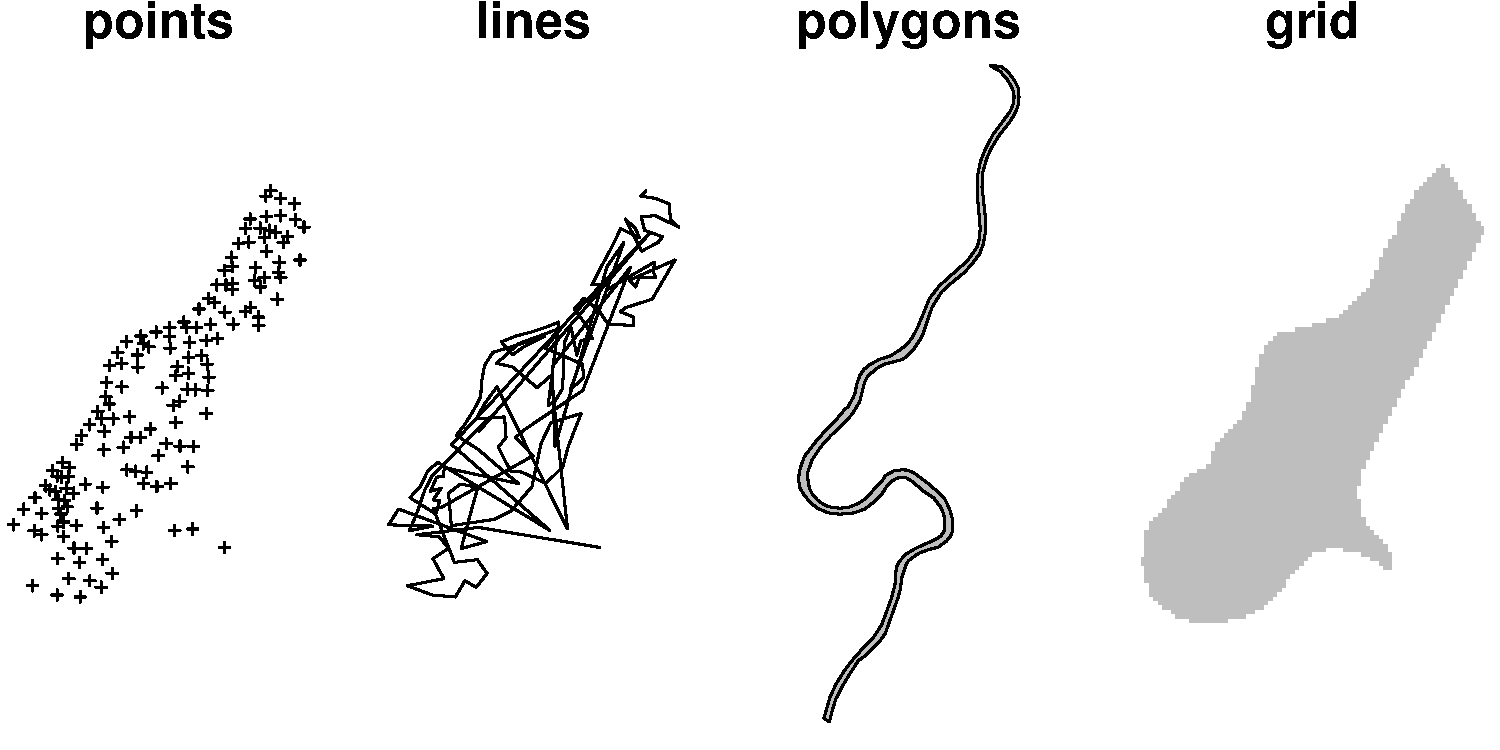
\includegraphics[width=0.7\columnwidth]{sp_plot1.pdf}
\end{figure}
\end{onlyenv}

\begin{onlyenv}<3>
\begin{columns} 
\begin{column}{.4\textwidth}
\begin{figure}[ht] \vspace{-10pt}
  \centering 
  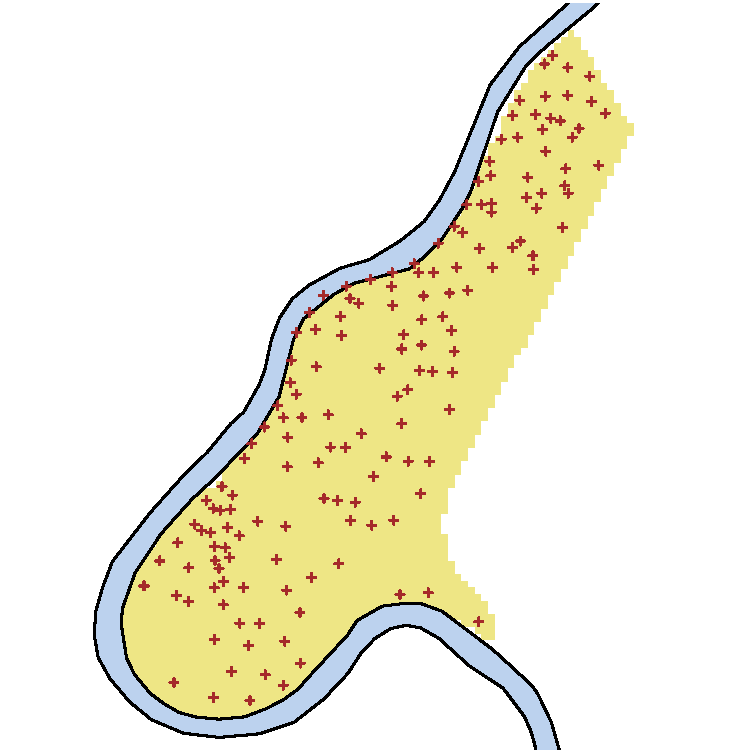
\includegraphics[width=\columnwidth]{sp_plot2.pdf}
\end{figure}
\end{column}

\begin{column}{.6\textwidth}
\centering
\begin{rcode}
# 创建一个绘图对象用于绘制空间网格对象
> image(meuse.grid, col = "khaki2")
# 在已有绘图对象上叠加空间面对象
> plot(meuse.pol, col = "lightsteelblue2", |\colorbox{green}{add = TRUE}|)
# 在已有绘图对象上叠加空间点对象
> plot(meuse, col = "brown", cex = .5, |\colorbox{green}{add = TRUE}|)
\end{rcode}
\end{column}
\end{columns}
\end{onlyenv}
\end{overlayarea}
\end{frame}

\subsubsection{绘制坐标轴和布局控制}
\begin{frame}[t,fragile]{\subsecname}{\subsubsecname}
\begin{itemize} 
\item<1-> 地图制图习惯不添加坐标轴,但是在\emphText{为了空间数据能够更易于阅读和统计分析},plot函数可以设置参数
\emphText{axes=TRUE}绘制默认坐标轴,坐标取值范围即bbbox值
\item<2-> 基础绘图系统\emphText{par}函数的参数也同样可以控制空间对象绘图
\end{itemize}

\begin{overlayarea}{\textwidth}{\textheight}
\begin{onlyenv}<1>
\begin{rcode}
# axes=TRUE绘制默认坐标轴
> plot(meuse.pol, |\colorbox{green}{axes = TRUE}|)
> title("add=TRUE",cex.main=2)
> plot(meuse.pol, |\colorbox{green}{axes = FALSE}|)
# axes=FALSE,可以用axis函数设置自定义坐标轴,包括刻度取值、刻度位置和字体大小等
> |\colorbox{green}{axis}|(1, at = c(178000 + 0:2 * 2000), cex.axis = .7) # 设置x轴
> |\colorbox{green}{axis}|(2, at = c(326000 + 0:3 * 4000), cex.axis = .7) # 设置y轴
> title("自定义坐标轴",cex.main=2); box()
\end{rcode}
\begin{figure}[ht] \vspace{-10pt}
  \centering 
  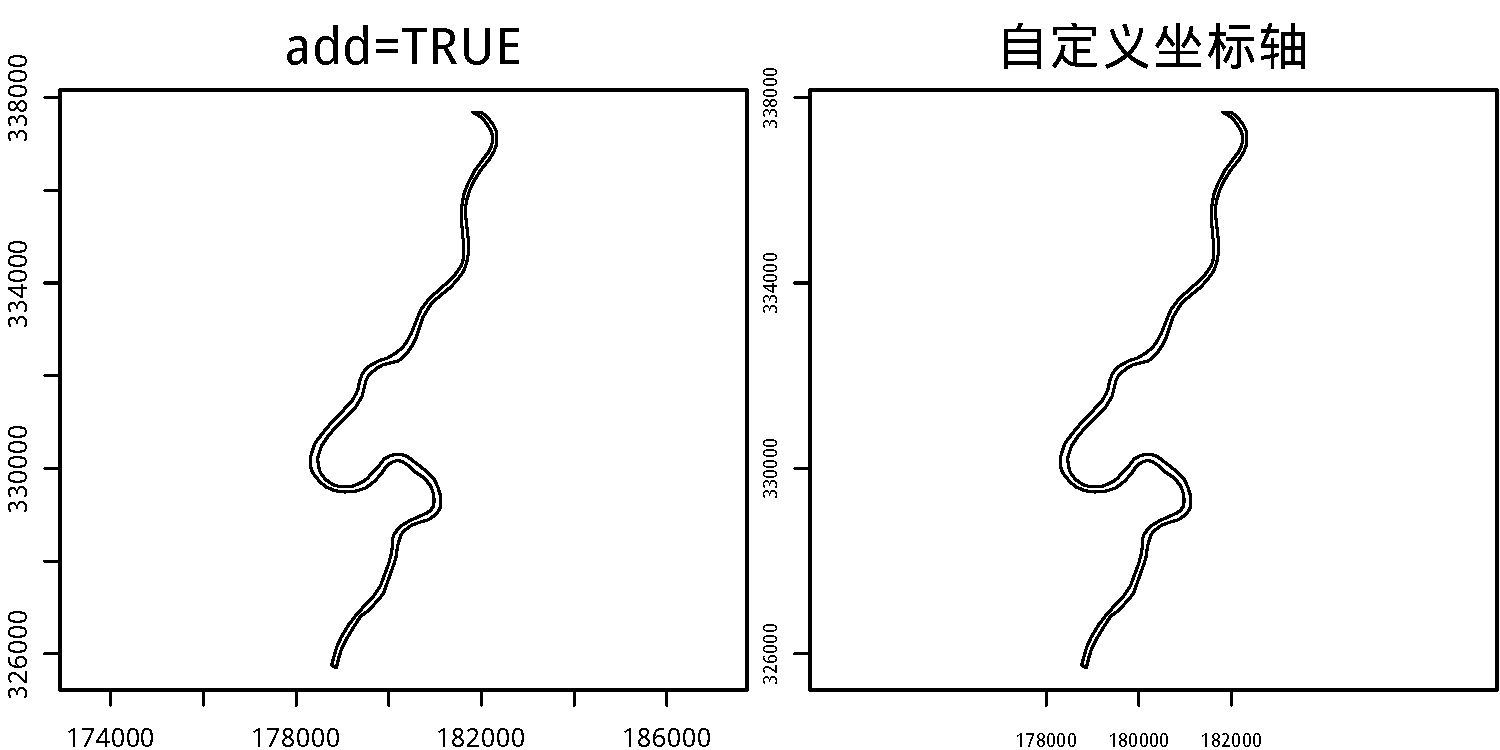
\includegraphics[width=0.75\columnwidth]{sp_axis1.pdf}
\end{figure}
\end{onlyenv}

\begin{onlyenv}<2>
\begin{rcode}
> oldpar = par(no.readonly = TRUE) # 保存par的默认参数
> layout(matrix(c(1,2),1,2))
> plot(meuse, axes = TRUE, cex = 0.6)
> plot(meuse.pol, add = TRUE)
> title("示例位置",cex.main=2)
# 用par函数mar参数控制绘图边框
> |\colorbox{green}{par(mar=c(0,0,0,0)+.1)}|
> plot(meuse, axes = FALSE, cex = 0.6)
> plot(meuse.pol, add = TRUE); box()
> par(oldpar) # 绘图完成后恢复默认参数
\end{rcode}
\begin{figure}[ht] \vspace{-10pt}
  \centering 
  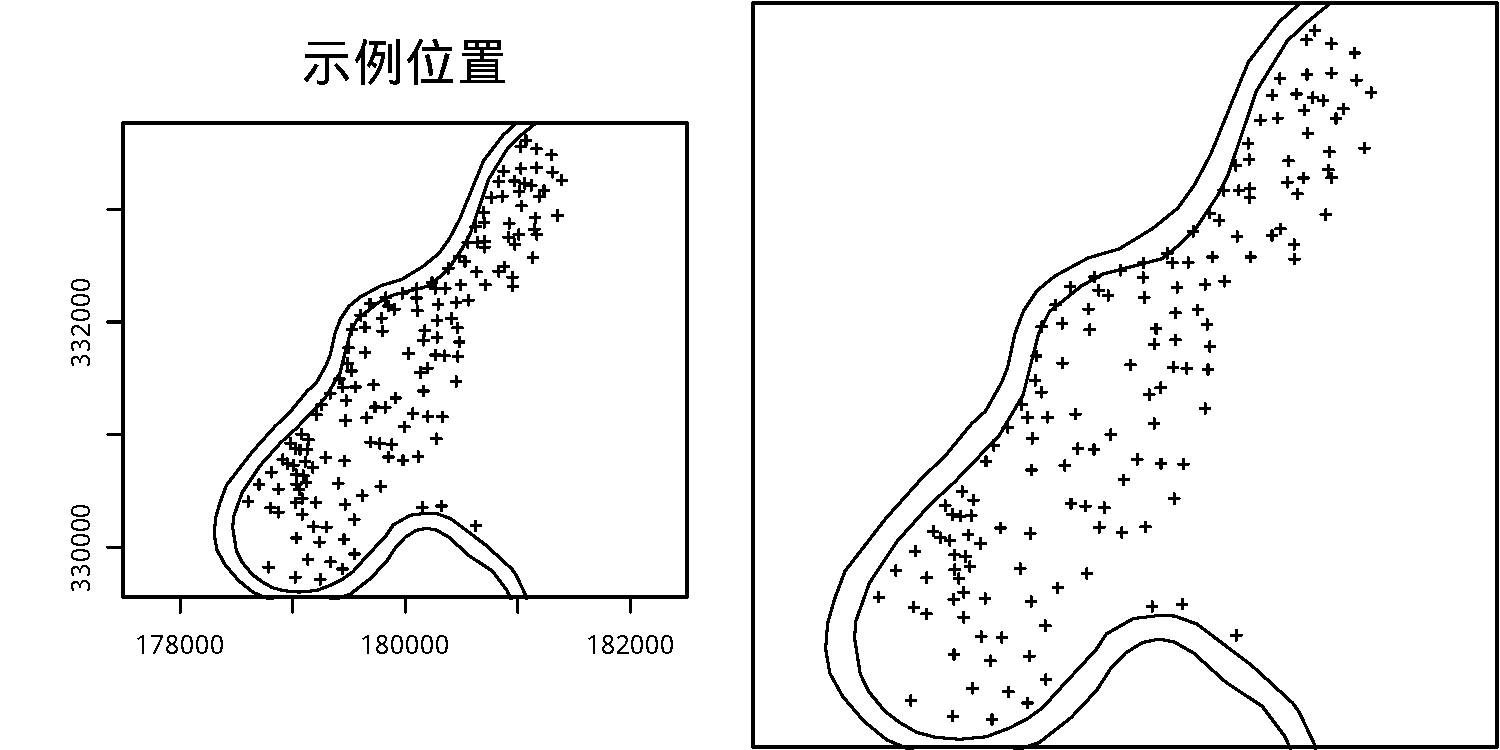
\includegraphics[width=0.7\columnwidth]{sp_axis2.pdf}
\end{figure}
\end{onlyenv}
\end{overlayarea}
\end{frame}

\subsubsection{绘制地图元素}
\begin{frame}[t,fragile]{\subsecname}{\subsubsecname}
\begin{itemize} 
\item<1-> \emphText{SpatialPolygonsRescale}函数用于绘制指北针和比例尺
\item<2-> \emphText{degAxis}函数用于显示带N/S/E/W标记的十进制度坐标刻度
\item<3-> \emphText{gridlines}函数用于绘制辅助网格线
\end{itemize}

\begin{overlayarea}{\textwidth}{\textheight}
\begin{onlyenv}<1>
\begin{rcode}
> plot(meuse); plot(meuse.pol, add=TRUE); box()
# 绘制比例尺:offset参数设置比例尺位置,scale设置比例尺尺度,fill设置填充颜色
> |\colorbox{green}{SpatialPolygonsRescale}|(|\colorbox{green}{layout.scale.bar()}|, offset = c(180200,329600), scale = 1000, fill = c("transparent","black"), plot.grid = FALSE)
> text(x = c(180200,181200), y = rep(329750, 2), c("0", "1 km")) # 比例尺显示文字
# 绘制指北针
> |\colorbox{green}{SpatialPolygonsRescale}|(|\colorbox{green}{layout.north.arrow()}|,offset=c(178750,332500),scale = 400,plot.grid = FALSE)
\end{rcode}
\begin{figure}[ht] \vspace{-5pt}
  \centering 
  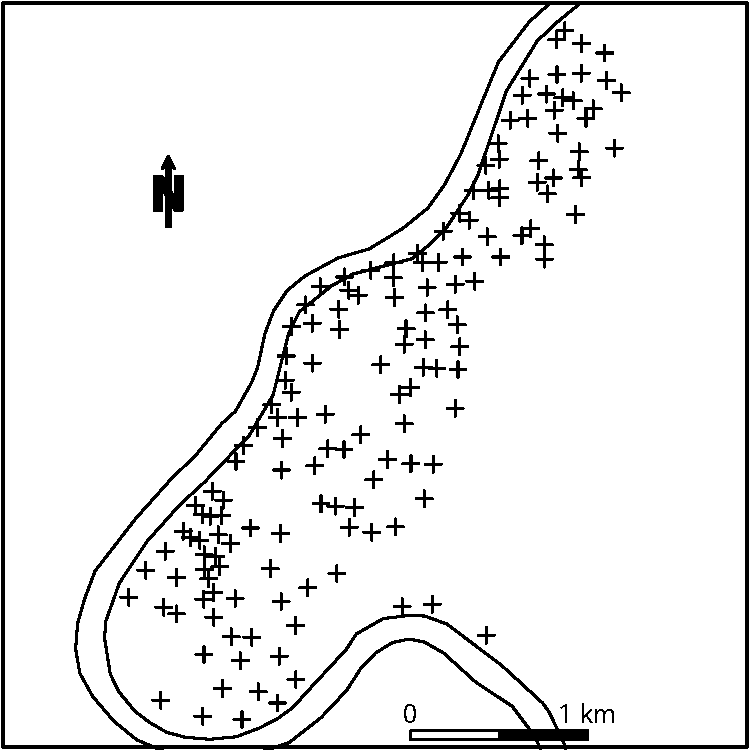
\includegraphics[width=0.4\columnwidth]{sp_mapelement1.pdf}
\end{figure}
\end{onlyenv}

\begin{onlyenv}<2>
\begin{rcode}
# 读取外部矢量地图数据
> nc <- readOGR(dsn=system.file("shapes",package="maptools"),layer="sids")
> proj4string(nc) <- CRS("+proj=longlat +datum=NAD27")
> rrt <- nc$SID74/nc$BIR74
> brks <- quantile(rrt, seq(0,1,1/5))
> library(RColorBrewer)
> cols <- brewer.pal(5, "Reds")
> plot(nc, col=cols[findInterval(rrt, brks, all.inside=TRUE)], axes = FALSE); box()
> |\colorbox{green}{degAxis}|(1) # 设置x轴
> |\colorbox{green}{degAxis}|(2, at=34:37) # 设置y轴
\end{rcode}
\begin{figure}[ht] \vspace{-10pt}
  \centering 
  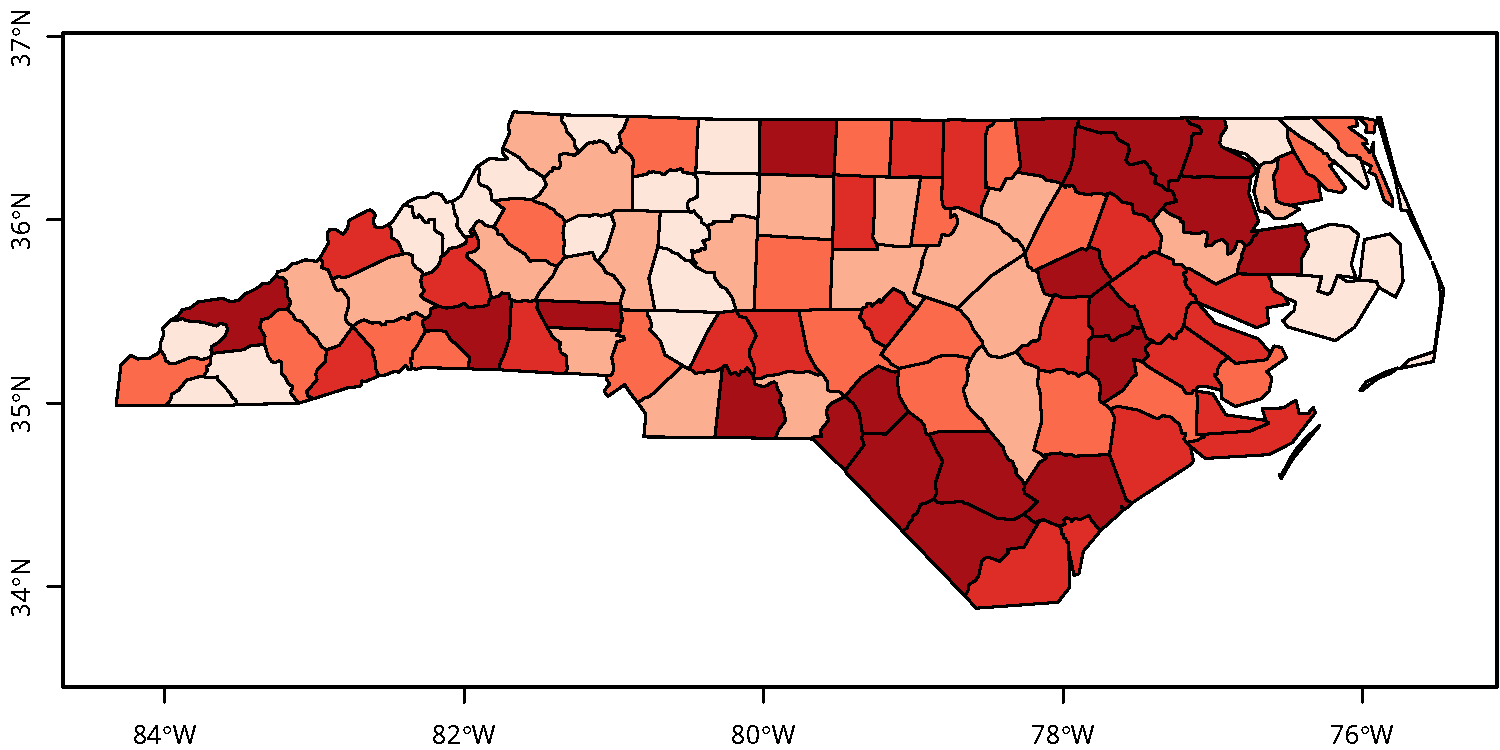
\includegraphics[width=0.75\columnwidth]{sp_mapelement2.pdf}
\end{figure}
\end{onlyenv}

\begin{onlyenv}<3>
\begin{rcode}
# 绘制世界地图和辅助网格线
> wrld <- map("world", interior=FALSE, xlim=c(-179,179), 
+    ylim=c(-89,89), plot=FALSE)
> wrld_p <- pruneMap(wrld, xlim=c(-179,179))
> llCRS <- CRS("+proj=longlat +ellps=WGS84")
> wrld_sp <- map2SpatialLines(wrld_p, proj4string=llCRS)
> prj_new <- CRS("+proj=moll +ellps=WGS84")
# 空间数据地图投影
> wrld_proj <- spTransform(wrld_sp, prj_new)
# 绘制GCS下的网格线: easts和norths设置东西和南北向坐标取值,ndiscr设置网格线离散点的数量
> wrld_grd <- |\colorbox{green}{gridlines}|(wrld_sp, easts=c(-179,seq(-150,150,50), 179.5),        norths=seq(-75,75,15), ndiscr=100)
# 网格线地图投影
> wrld_grd_proj <- spTransform(wrld_grd, prj_new)
# 显示GCS下网格线刻度文字:side参数可以设置显示文字的侧面,默认只在西侧和南侧显示文字
> at_sp <- |\colorbox{green}{gridat}|(wrld_sp, easts=0, norths=seq(-75,75,15), offset=0.3)
# 网格线刻度文字地图投影
> at_proj <- spTransform(at_sp, prj_new)
> plot(wrld_proj, col="grey60")
> plot(wrld_grd_proj, add=TRUE, lty=3, col="grey70")
# 使用投影计算后的位置显示文字
> text(coordinates(at_proj), |\colorbox{green}{pos=at\_proj\$pos}|, offset=at_proj$offset,labels=parse(text=as.character(at_proj$labels)), cex=1)
\end{rcode}
\end{onlyenv}

\only<4>{
\begin{figure}[ht] \vspace{-5pt}
  \centering 
  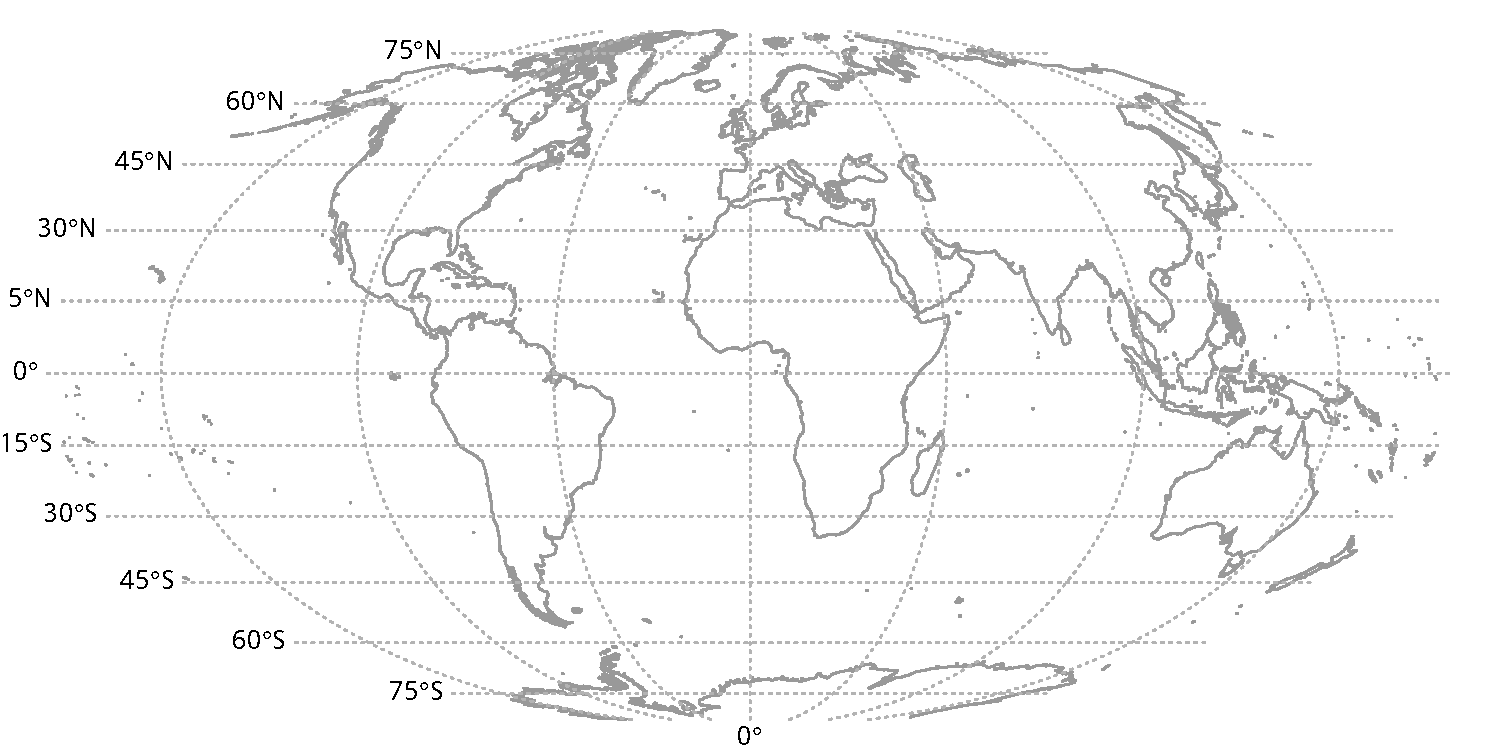
\includegraphics[width=\columnwidth]{sp_mapelement3.pdf}
\end{figure}}
\end{overlayarea}
\end{frame}

\begin{frame}[t,fragile]{\subsecname}{\subsubsecname}
\begin{itemize} 
\item<1-> 绘图函数的\emphText{pch}、\emphText{lwd}等参数用于绘制空间图形要素的颜色、样式等属性,用法和对应的普通图形要素绘制类似
\item<2-> \emphText{legend}函数用于绘制地图图例
\end{itemize}

\begin{overlayarea}{\textwidth}{\textheight}
\only<1>{ 
  \begin{table} \centering \small
    \renewcommand\arraystretch{0.6} 
    \begin{tabular}{|>{\centering\arraybackslash} m{0.4\columnwidth} |>{\centering\arraybackslash} m{0.1\columnwidth} |>{\centering\arraybackslash} m{0.2\columnwidth} |>{\centering\arraybackslash} m{0.15\columnwidth}|}
      \toprule
      \rowcolor{LightCyan}
      \multicolumn{1}{|c|}{\textbf{空间类}} & \multicolumn{1}{c|}{\textbf{参数}} 
& \multicolumn{1}{c|}{\textbf{含义}} & \multicolumn{1}{c|}{\textbf{帮助}} \\\hline

\multirowcell{4}{SpatialPointsDataFrame} & pch & 样式 & \multirowcell{4}{?points} \\
& col & 颜色 & \\
& bg & 填充色 & \\
& cex & 大小 & \\\hline
\multirowcell{3}{SpatialLinesDataFrame} & col & 颜色 & \multirowcell{3}{?lines} \\
& lwd & 线宽 & \\
& lty & 线型 & \\\hline
\multirowcell{5}{SpatialPolygonsDataFrame} & border & 边框颜色 & \multirowcell{5}{?polygon} \\
& lty & 线类型 & \\
& pbg & 孔类型 & \\
& density & 填充线密度 & \\
& angle & 填充线角度 & \\\hline
\multirowcell{3}{SpatialGridsDataFrame\\ SpatialPixelsDataframe} & zlim & 属性值范围 & \multirowcell{3}{?image} \\
& col & 颜色 & \\
& breaks & 分级断点 & \\\hline
      \bottomrule
    \end{tabular}
    \caption{基础绘图系统绘图函数中用于绘制空间图形要素的主要参数}
  \end{table}}

\begin{onlyenv}<2>
\begin{columns} 
\begin{column}{.4\textwidth}
\begin{figure}[ht] \vspace{-10pt}
  \centering 
  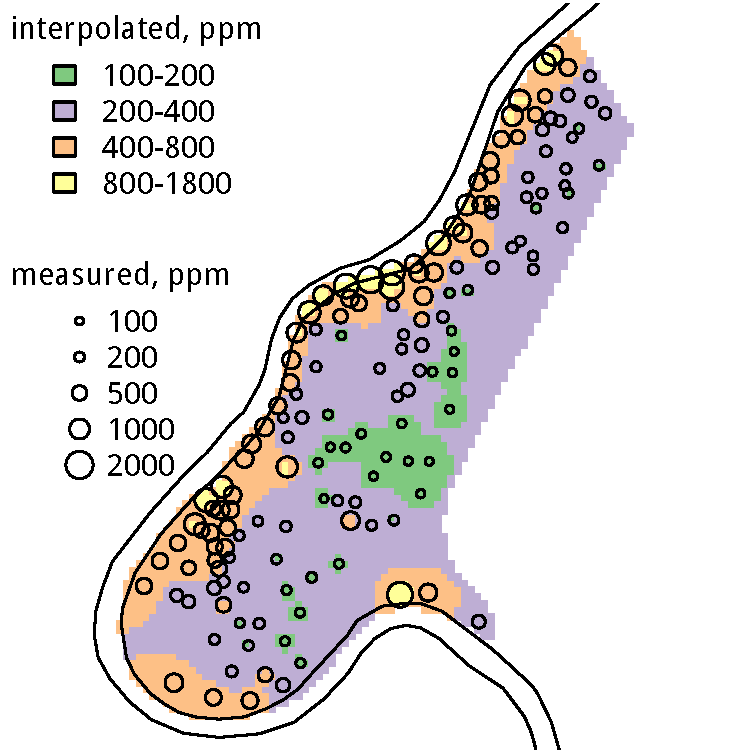
\includegraphics[width=\columnwidth]{sp_mapelement4.pdf}
\end{figure}
\end{column}

\begin{column}{.6\textwidth}
\centering
\begin{rcode}
> library(RColorBrewer)
> cols <- brewer.pal(4, "Accent") # 分四个等级
# 设置空间图形要素
> image(zn.idw, |\colorbox{green}{col}| = cols, |\colorbox{green}{breaks}|=log(c(100,200,400,800,1800)))
> plot(meuse.pol, add = TRUE)
> plot(meuse,|\colorbox{green}{pch}|=1,|\colorbox{green}{cex}|=sqrt(meuse$zinc)/20,add=TRUE)
# 绘制空间要素的图例
> |\colorbox{green}{legend}|("left", legend=c(100, 200, 500, 1000, 2000), pch = 1, pt.cex = sqrt(legVals)/20, bty = "n", title="measured, ppm", cex=1.2, y.inter=1)
> |\colorbox{green}{legend}|("topleft", fill = cols, legend=c("100-200","200-400","400-800","800-1800"), bty = "n", title = "interpolated, ppm", cex=1.2, y.inter=1)
\end{rcode}
\end{column}
\end{columns}
\end{onlyenv}
\end{overlayarea}
\end{frame}

\subsubsection{绘图交互}
\begin{frame}[t,fragile]{\subsecname}{\subsubsecname}
\begin{itemize} 
\item<1-> 地图要素在绘图区域的定位可以在程序中设置绝对数值来完成,也可以用R的交互函数通过鼠标点击手动完成
\item<2-> 相比GIS软件,R的交互功能比较弱,只提供了两个交互函数\emphText{locator}和\emphText{identify},两者
都会等待鼠标输入,单击左键开始,单击右键结束
\item<2-> locator函数返回单击的坐标位置,identify函数在一个指定距离范围内绘制并返回离点击位置
最近的标签值
\end{itemize}

\begin{overlayarea}{\textwidth}{\textheight}
\begin{onlyenv}<2>
\begin{rcode}
> plot(meuse,axes=FALSE)
> plot(meuse.pol, add=TRUE)
> box()
# 通过鼠标点击来定位比例尺、指北针以及说明文字的位置;相对绝对数值,这种定位方式不够精准,但是比较直观
> SpatialPolygonsRescale(layout.scale.bar(), offset = |\colorbox{green}{locator(1)}|, scale = 1000, fill=c("transparent","black"), plot.grid = FALSE)
> text(|\colorbox{green}{locator(1)}|, "0")
> text(|\colorbox{green}{locator(1)}|, "1 km")
> SpatialPolygonsRescale(layout.north.arrow(), offset = |\colorbox{green}{locator(1)}|, scale = 400, plot.grid = FALSE)
\end{rcode}
\end{onlyenv}
\end{overlayarea}
\end{frame}

\subsection{基于lattice的绘图方法}
\subsubsection{spplot函数}
\begin{frame}[t,fragile]{\subsecname}{\subsubsecname}
\begin{itemize} 
\item<1-> sp包基于Spatial类封装了lattice包的绘图函数,实现在grid绘图系统中绘制空间数据,对应的绘图函数是
\emphText{spplot}函数
\item<1-> spplot的返回值是trellis对象,\emphText{大部分参数和xyplot函数通用}
\item<2-> spplot函数通过\emphText{接收GIS属性数据}实现便捷的绘图方式,
每个panel绘制一个属性,多个属性则自动生成多个panel
\end{itemize}

\begin{overlayarea}{\textwidth}{\textheight}
\begin{onlyenv}<2>
\begin{rcode}
# 为meuse数据集挂载四个属性
> data(meuse)
> coordinates(meuse) <- ~x+y
> meuse$lead.st = as.vector(scale(meuse$lead))
> meuse$zinc.st = as.vector(scale(meuse$zinc))
> meuse$copper.st = as.vector(scale(meuse$copper))
> meuse$cadmium.st = as.vector(scale(meuse$cadmium))
# 设置指北针和比例尺
> l2 = list("SpatialPolygonsRescale", layout.north.arrow(), offset = c(178750,332500), scale = 400)
> l3 = list("SpatialPolygonsRescale", layout.scale.bar(), offset = c(180500,329800), scale = 500, fill=c("transparent","black"))
> l4 = list("sp.text", c(180500,329900), "0")
> l5 = list("sp.text", c(181000,329900), "500 m")
# 定义分级断点
> cuts=c(-1.2,0,1,2,3,5)
# 设置颜色等级
> grys <- brewer.pal(7, "Reds")
# spplot函数绘制meuse数据集的四个属性:第一个参数是空间数据集,第二个参数是需要绘制的属性,sp.layout参数设置地图要素,col.regions参数设置颜色等级,其他参数和xyplot函数通用
> |\colorbox{green}{spplot}|(meuse, c("cadmium.st", "copper.st", "lead.st", "zinc.st"),
        |\colorbox{green}{sp.layout}|=list(l2,l3,l4,l5), layout=c(2,2),
        key.space="right", main=list("标准差",), 
        par.strip.text=list(cex=2), aspect=1,
        cuts = cuts,|\colorbox{green}{col.regions}|=grys)
\end{rcode}
\end{onlyenv}

\begin{onlyenv}<3>
\begin{figure}[ht] \vspace{-20pt}
  \centering 
  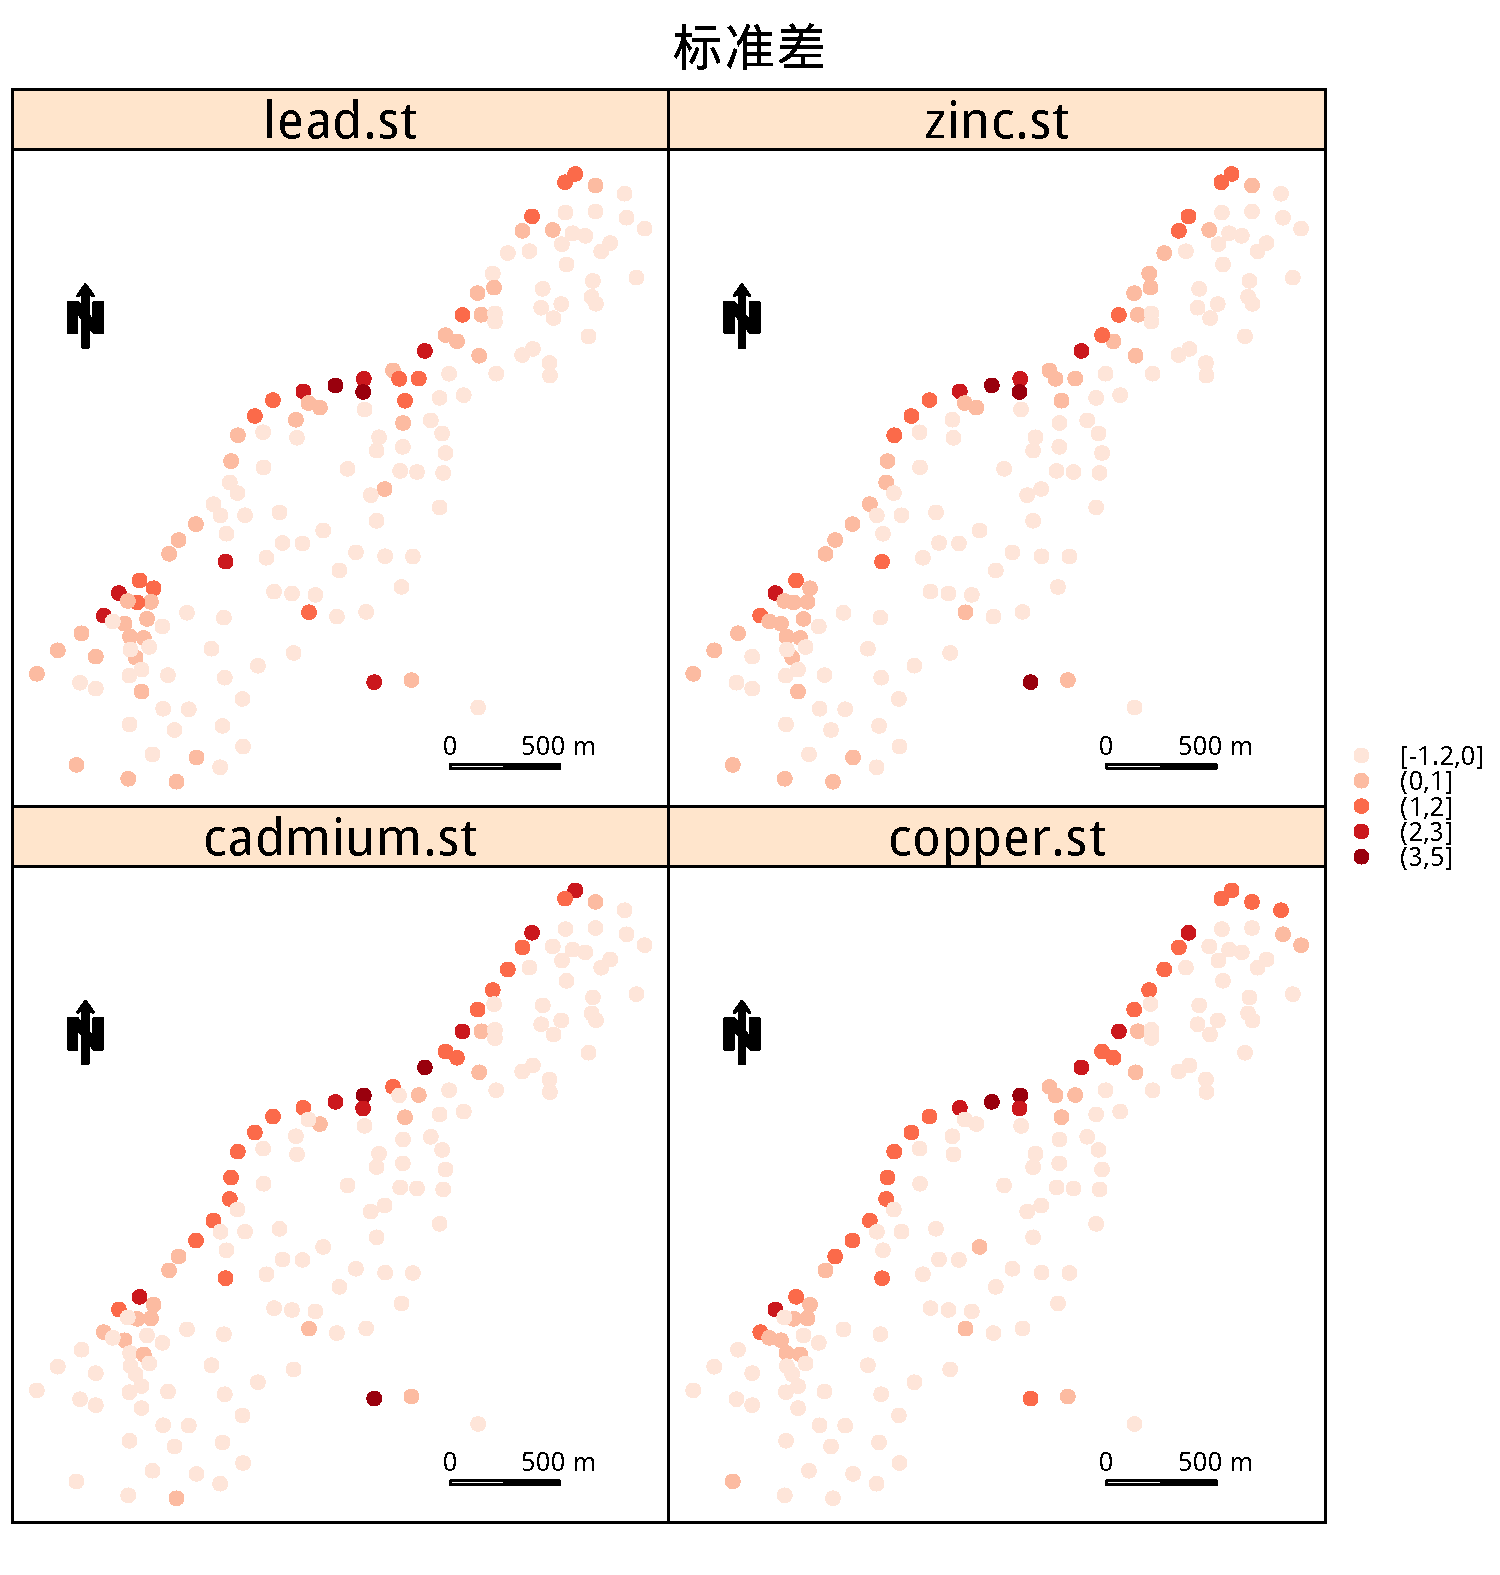
\includegraphics[width=0.5\columnwidth]{spplot1.pdf}
\end{figure}
\end{onlyenv}
\end{overlayarea}
\end{frame}

\subsubsection{添加布局项}
\begin{frame}[t,fragile]{\subsecname}{\subsubsecname}
\begin{itemize} 
\item<1-> \emphText{sp.layout}参数用来添加点、线、面、文本等基本绘图要素以及地图要素,
这个参数\emphText{接收一个由布局项构成的list对象},其中布局项本身也是一个list对象且第一个参数是函数名称
\end{itemize}

\begin{overlayarea}{\textwidth}{\textheight}
\only<1>{
\begin{table} \centering \scriptsize
    \renewcommand\arraystretch{1}
    \begin{tabular}{>{\centering\arraybackslash} m{0.3\columnwidth} >{\centering\arraybackslash} m{0.2\columnwidth} >{\centering\arraybackslash} m{0.3\columnwidth}}
      \toprule
      \rowcolor{LightCyan}
      \multicolumn{1}{c}{\textbf{sp布局函数}} & \multicolumn{1}{c}{\textbf{类型}} & \multicolumn{1}{c}{\textbf{主要参数}}\\\hline
      sp.points & SpatialPoints & pch,cex.col \\
      sp.polygons & SpatialPolygons & lty,lwd,col\\
      sp.lines & SpatialLines & lty,lwd,col\\
      sp.text & text & col,cex,srt\\\hline
      \bottomrule
    \end{tabular}
    \caption{sp包的布局函数,其作为list对象的一部分被sp.layout参数接收,
函数参数与par相同,可以用?par查看相关参数说明}
\end{table}}

\begin{onlyenv}<2>
\begin{rcode}
# 布局函数list对象按类型组成需要添加的绘图要素,这与基本绘图系统是类似的,但是实现上更为优雅
> river <- list("sp.polygons", meuse.pol)
# 这里除了基本绘图要素外,还可以添加地图要素
> north <- list("SpatialPolygonsRescale", layout.north.arrow(), offset = c(178750,332500), scale = 400)
> scale <- list("SpatialPolygonsRescale", layout.scale.bar(), offset = c(180200, 329800), scale = 1000, fill=c("transparent","black"))
> txt1 <- list("sp.text", c(180200, 329950), "0")
> txt2 <- list("sp.text", c(181200, 329950), "1 km")
> pts <- list("sp.points", meuse, pch = 3, col = "black")
# 最后所有布局项组成一个list对象传入sp.layout参数,并用于最终的绘图
> |\colorbox{green}{meuse.layout <- list(river, north, scale, txt1, txt2, pts)}|
> grys <- brewer.pal(7, "Reds")
> spplot(zn["log"], |\colorbox{green}{sp.layout = meuse.layout}|, cuts=5, col.regions=grys)
\end{rcode}
\end{onlyenv}

\begin{onlyenv}<3>
\begin{figure}[ht] \vspace{-20pt}
  \centering 
  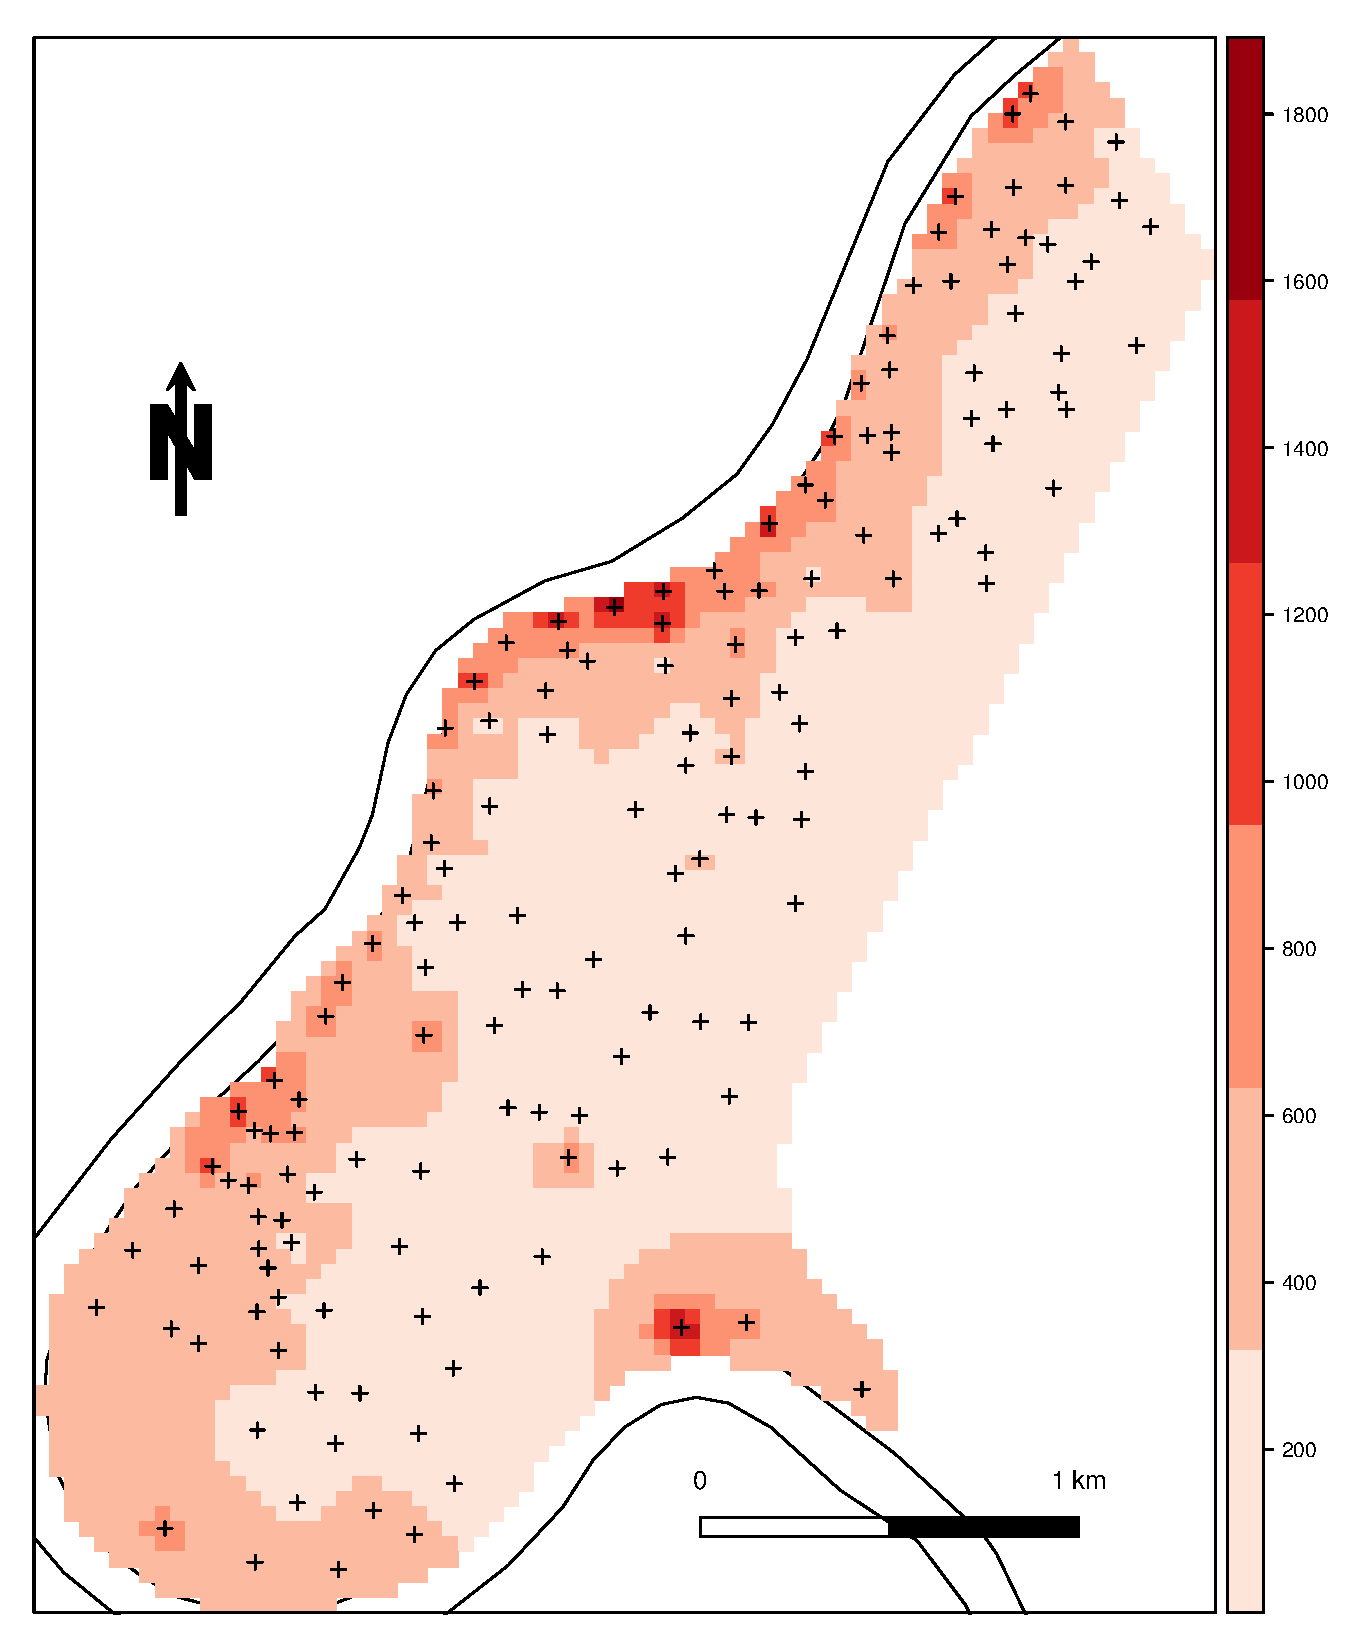
\includegraphics[width=0.5\columnwidth]{spplot2.pdf}
\end{figure}
\end{onlyenv}
\end{overlayarea}
\end{frame}

\subsubsection{panel排列布局}
\begin{frame}[t,fragile]{\subsecname}{\subsubsecname}
\begin{itemize} 
\item<1-> 相比plot函数,spplot函数最大的优势是可以
\emphText{在同一绘图区域不同panel对多个属性绘图},从而实现分析结果的比较
\item<1-> panel的排列布局通过\emphText{layout}和\emphText{skip}参数实现;layout设置panel排列的行列数,skip则设置需要留白的panel
\end{itemize}

\begin{overlayarea}{\textwidth}{\textheight}
\begin{onlyenv}<2>
  \begin{figure} \vspace{-10pt}
    \begin{columns}
      \begin{column}{.6\textwidth}
        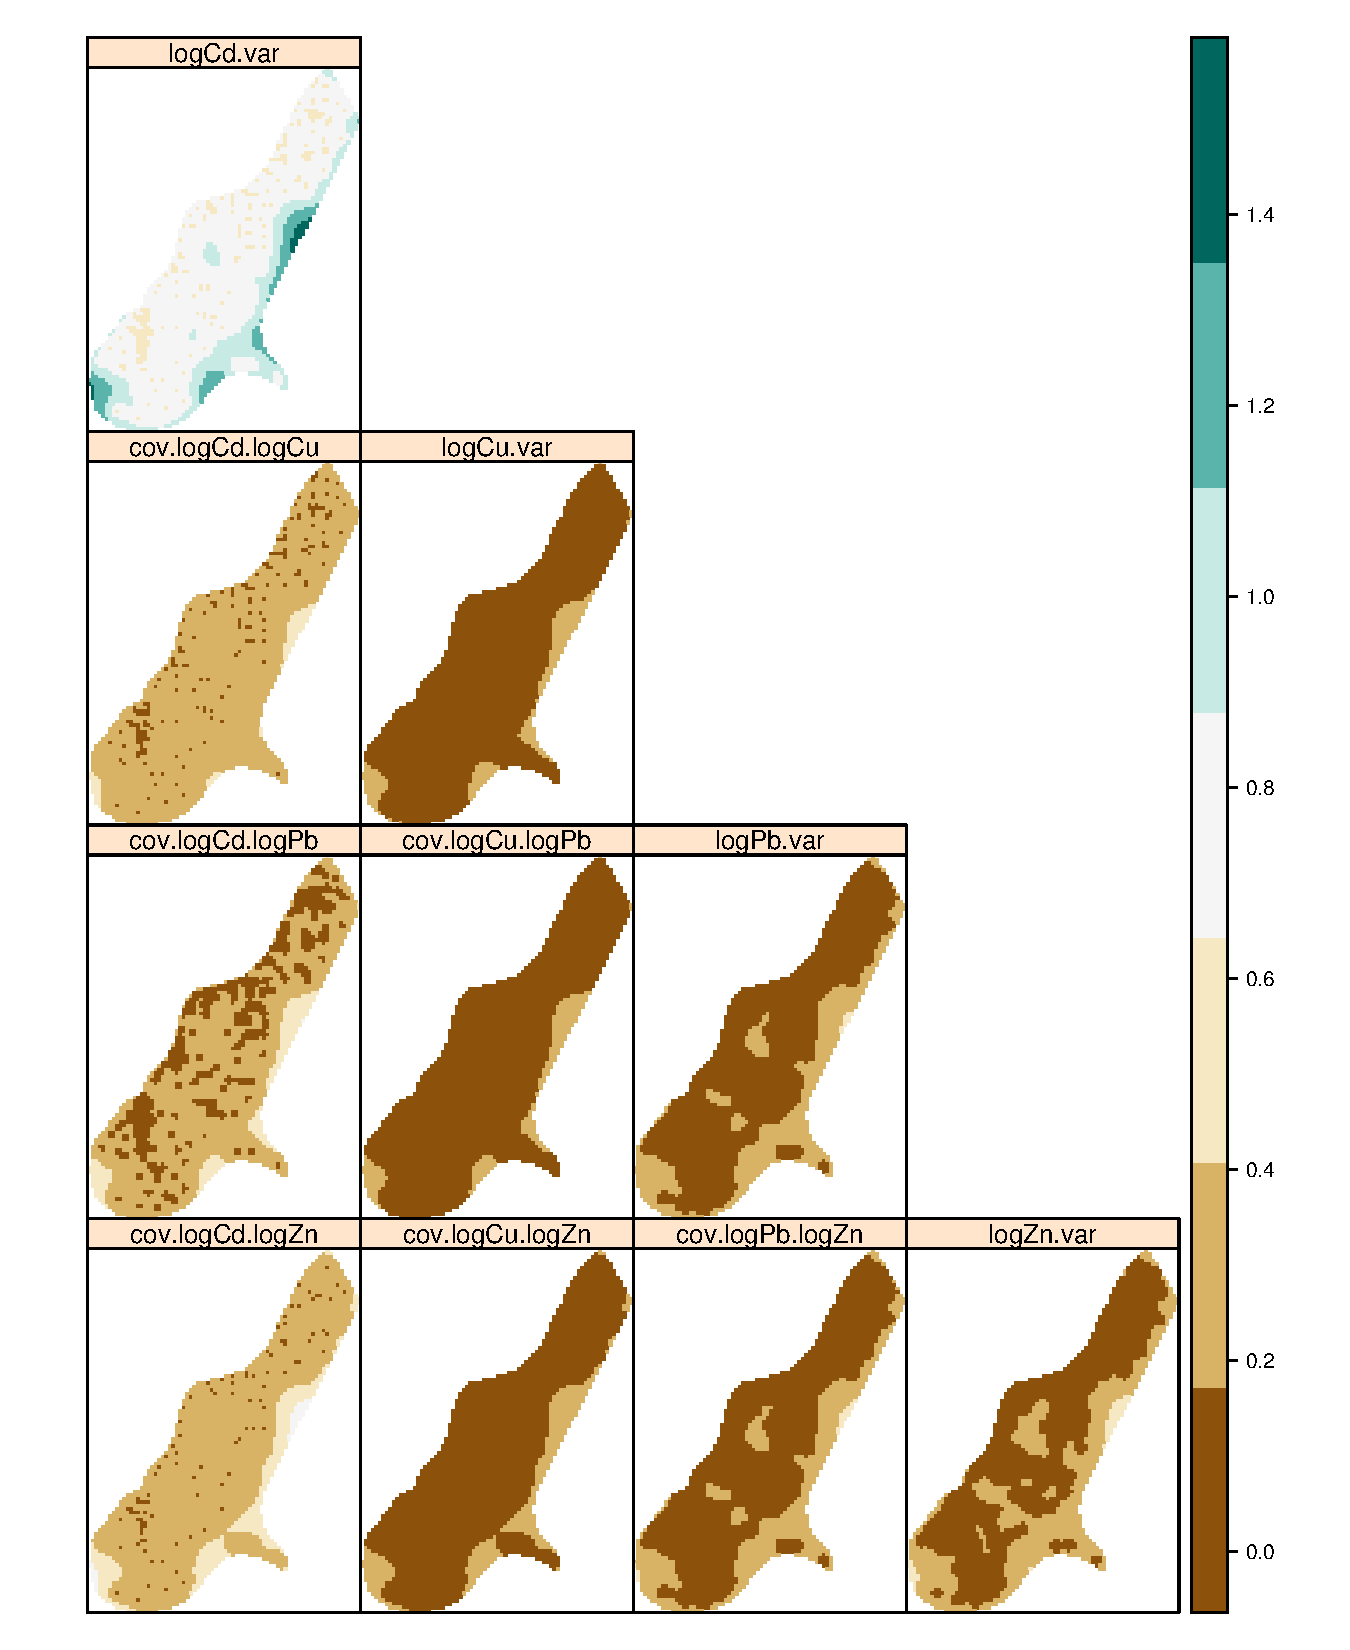
\includegraphics[width=0.8\columnwidth]{spplot3.pdf}
      \end{column}
       \hspace{-40pt}    
      \begin{column}{.4\textwidth}
 \caption{协克里金方差矩阵的统计图形展示,参数为layout=c(4,4),\\skip=c(F,T,T,T,F,F,T,T,F,\\F,F,T,T,T,T,T)}
      \end{column}
    \end{columns}
  \end{figure}
\end{onlyenv}
\end{overlayarea}
\end{frame}

\subsection{基于ggplot2的绘图方法}
\subsubsection{绘制矢量空间数据}
\begin{frame}[t,fragile]{\subsecname}{\subsubsecname}
\begin{itemize} 
\item<1-> sp包没有重新编写基于ggplot2包的绘图函数,但是空间点对象可以直接转换为data.frame,线和面则利用ggplot2包的\emphText{fortify}函数转换为data.frame,然后再用绘图函数绘图
\item<5-> 利用ggplot2的\emphText{分面函数}在同一图幅中展示数据的不同类别
\end{itemize}

\begin{overlayarea}{\textwidth}{\textheight}
\begin{onlyenv}<1>
\begin{rcode}
# ggplot2包提供fortify函数将线和面空间对象转换为data.frame
> methods(fortify)
 [1] fortify.cld*                      fortify.confint.glht*            
 [3] fortify.data.frame*               fortify.default*                 
 [5] fortify.function*                 fortify.glht*                    
 [7] fortify.Line*                     fortify.Lines*                   
 [9] fortify.lm*                       fortify.map*                     
[11] fortify.NULL*                     fortify.Polygon*                 
[13] fortify.Polygons*                 |\colorbox{green}{fortify.SpatialLinesDataFrame*}|   
[15] |\colorbox{green}{fortify.SpatialPolygons*}|          |\colorbox{green}{fortify.SpatialPolygonsDataFrame*}|
[17] fortify.summary.glht*            
see '?methods' for accessing help and source code
\end{rcode}
\end{onlyenv}

\begin{onlyenv}<2>
\begin{columns} 
\begin{column}{.4\textwidth}
\begin{figure}[ht] \vspace{-10pt}
  \centering 
  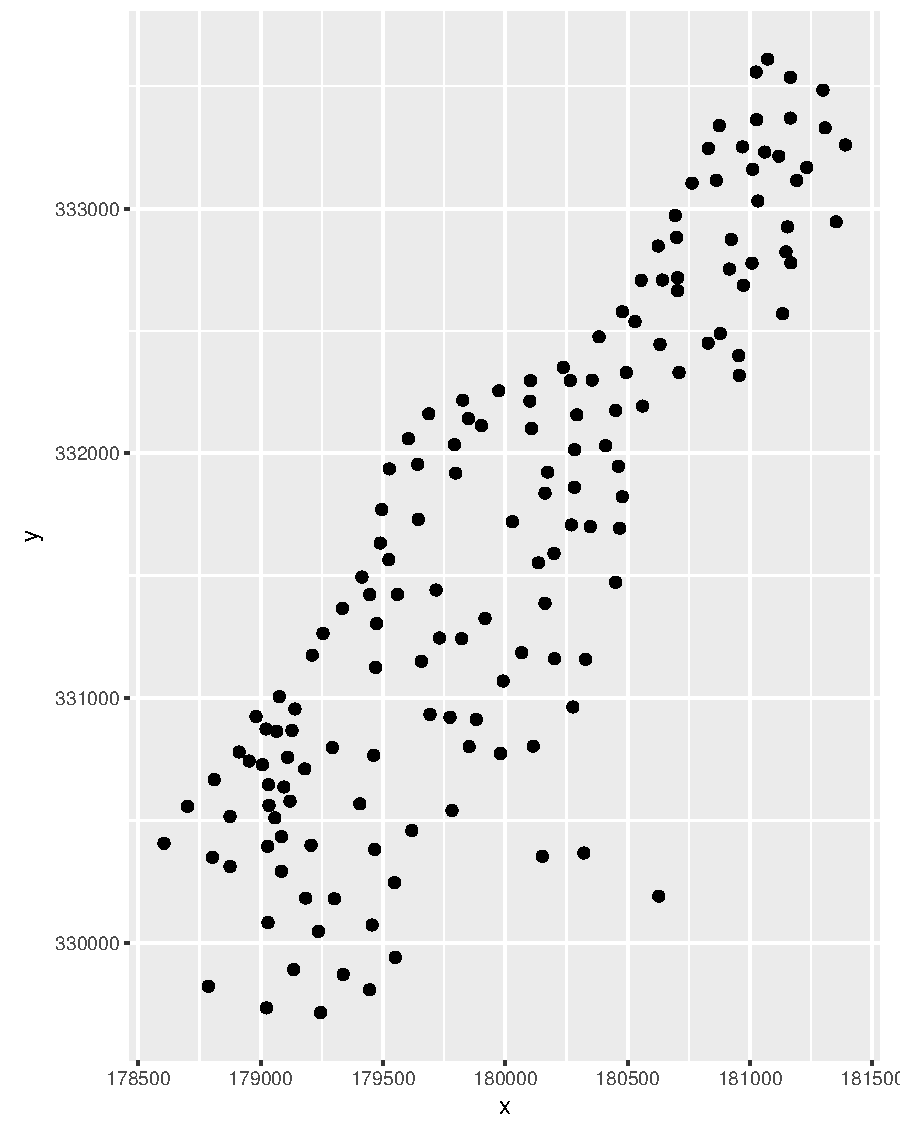
\includegraphics[width=\columnwidth]{spggplot1.pdf}
\end{figure}
\end{column}

\begin{column}{.6\textwidth}
\centering
\begin{rcode}
> data(meuse)
> coordinates(meuse) <- ~x+y
# 将空间点对象转换为data.frame对象
> m <- |\colorbox{green}{as}|(meuse,"data.frame")
# 用ggplot函数绘图
> ggplot(m, aes(x, y))+geom_point()+coord_equal()
\end{rcode}
\end{column}
\end{columns}
\end{onlyenv}

\begin{onlyenv}<3>
\begin{rcode}
# 读取一个面状shp图层,属性数据包括四个字段
> sport <- readOGR(dsn = "./data/", "london_sport")
> str(sport,max.level=2)
Formal class 'SpatialPolygonsDataFrame' [package "sp"] with 5 slots
  ..@ data       :'data.frame': 33 obs. of  4 variables:
  ..@ polygons   :List of 33
  ..@ plotOrder  : int [1:33] 1 3 4 19 10 25 28 2 7 27 ...
  ..@ bbox       : num [1:2, 1:2] 503571 155851 561941 200932
  .. ..- attr(*, "dimnames")=List of 2
  ..@ proj4string:Formal class 'CRS' [package "sp"] with 1 slot  
> str(sport@data,max.level=2)
'data.frame':   33 obs. of  4 variables:
 $ ons_label : Factor w/ 33 levels "00AA","00AB",..: 6 27 17 16 21 29 18 24 32 8 ...
 $ name      : Factor w/ 33 levels "Barking and Dagenham",..: 5 27 17 16 21 29 18 24 32 8 ...
 $ Partic_Per: num  21.7 26.6 21.5 17.9 24.4 19.3 16.9 20.7 26 17.6 ...
 $ Pop_2001  : Factor w/ 33 levels "147271","158921",..: 29 5 21 19 1 7 14 9 25 32 ...

# fortify函数将空间面对象转换为data.frame
> sport.f <- |\colorbox{green}{fortify}|(sport, region = "ons_label")
> sport.f <- merge(sport.f, sport@data, by.x = "id", by.y = "ons_label") # 挂载属性信息
> Map <- |\colorbox{green}{ggplot}|(sport.f, aes(long, lat, group = group, fill = Partic_Per)) + |\colorbox{green}{geom\_polygon}|() + |\colorbox{green}{geom\_path}|(colour="white",lwd=0.3) + coord_equal() + labs(x = "Easting (m)", y = "Northing (m)", fill = "% Sport Partic.") + ggtitle("London Sports Participation")
> Map + scale_fill_gradient(low = "green", high = "red")
\end{rcode}
\end{onlyenv}

\begin{onlyenv}<4>
\begin{figure}[ht] \vspace{-20pt}
  \centering 
  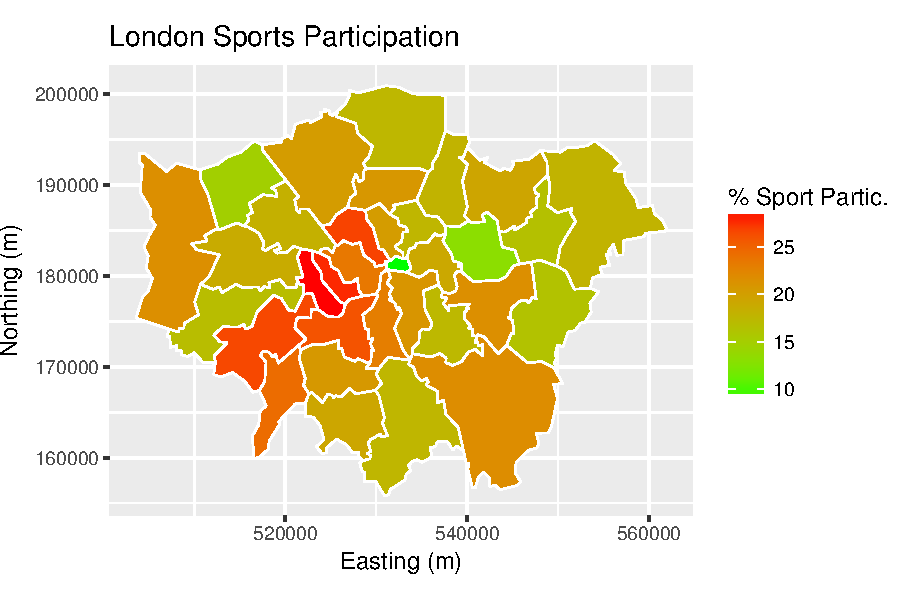
\includegraphics[width=0.8\columnwidth]{spggplot2.pdf}
\end{figure}
\end{onlyenv}

\begin{onlyenv}<5>
\begin{rcode}
> library(reshape2)
# 读取伦敦市各行政区历年人口数据
> london.data <- read.csv("data/census-historic-population-borough.csv")
# 将人口数据全部融合到data.frame的一列variable
> london.data.melt <- melt(london.data, id = c("Area.Code", "Area.Name"))
> plot.data <- merge(sport.f, london.data.melt, by.x = "id", by.y = "Area.Code")
# 用分面函数facet_wrap根据变量variable的不同类别绘图
> ggplot(data = plot.data, aes(x = long, y = lat, fill = value, group = group)) + 
         geom_polygon() + 
         geom_path(colour = "white", lwd = 0.3) + 
         coord_equal() + 
        |\colorbox{green}{facet\_wrap}|(~variable)
\end{rcode}
\end{onlyenv}

\begin{onlyenv}<6>
\begin{figure}[ht] \vspace{-20pt}
  \centering 
  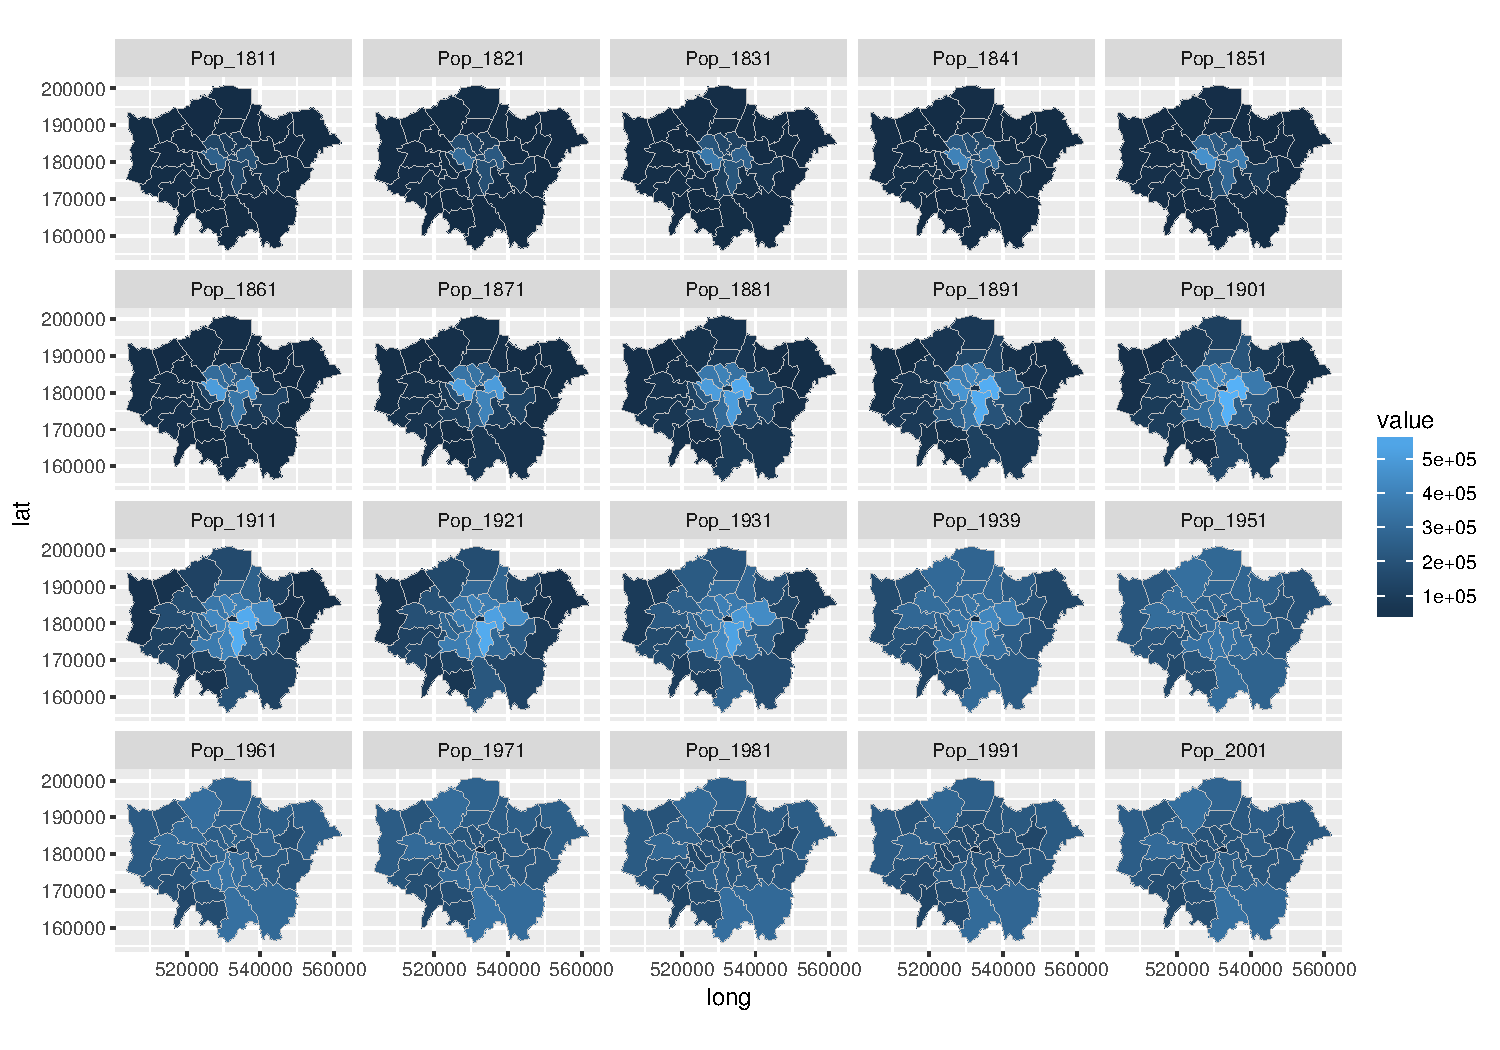
\includegraphics[width=0.8\columnwidth]{spggplot3.pdf}
\end{figure}
\end{onlyenv}
\end{overlayarea}
\end{frame}

\begin{frame}[t,fragile]{\subsecname}{\subsubsecname}
\begin{itemize} 
\item<1-> 除了间接转换的方法,ggplot2包在正在开发的新版本中提供了\emphText{gemo\_sf}函数可以直接绘制从
\emphText{sf包}读取的空间数据对象
\end{itemize}

\begin{overlayarea}{\textwidth}{\textheight}
\begin{onlyenv}<2>
\begin{rcode}
# 因为geom_sf函数还未正式发布,因此用install_github函数直接获取开发版源代码
> \|colorbox{green}{devtools::install\_github}|("tidyverse/ggplot2")
> require(ggplot2) # 重新加载开发版的ggplot2
# 用sf包读取空间矢量数据
> nc <- sf::st_read(system.file("shape/nc.shp", package = "sf"), quiet = TRUE)
> nc_3857 <- sf::st_transform(nc, "+init=epsg:3857") # 坐标系转换
> nc_3857$mid <- sf::st_centroid(nc_3857$geometry)  # 抽取面状要素的中心点
# 先绘制面层,再绘制点层
> ggplot(nc_3857) + 
+     |\colorbox{green}{geom\_sf}|(aes(fill = AREA), colour = "white", lwd = 0.5) +
+     |\colorbox{green}{geom\_sf}|(aes(geometry = mid, size = BIR74), show.legend = "point") 
\end{rcode}
\begin{figure}[ht] 
  \centering 
  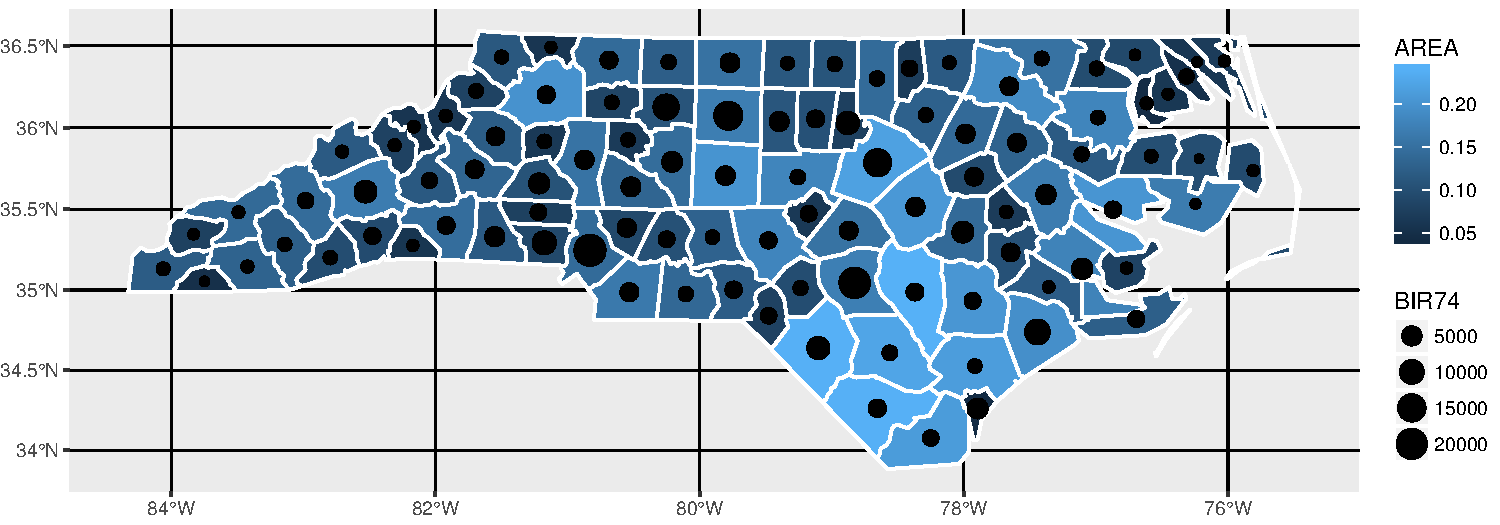
\includegraphics[width=\columnwidth]{spggplot4.pdf}
\end{figure}
\end{onlyenv}
\end{overlayarea}
\end{frame}

\subsubsection{绘制栅格空间数据}
\begin{frame}[t,fragile]{\subsecname}{\subsubsecname}
\begin{itemize} 
\item<1-> 栅格空间数据可以用ggplot2包的\emphText{geom\_raster}或\emphText{geom\_tile}函数直接绘制;\emphText{建议在栅格数据较大时采用geom\_raster函数}
\end{itemize}

\begin{overlayarea}{\textwidth}{\textheight}
\begin{onlyenv}<1>
\begin{rcode}
> library(viridis) # 这个包可以让输出的地图配色更专业 
> library(raster); library(reshape2)
# 从外部文件读取栅格数据,包括三个波段
> carmel_bay <- brick("data/carmel_bay_bathy.tif")
# 将RasterBrick对象转换成data.frame
> bay_spdf <- as(carmel_bay, "SpatialPixelsDataFrame")
> bay_df <- as.data.frame(bay_spdf)
> bay_df <- melt(bay_df, id=c("x","y")) # 将不同波段数据融合到data.frame的一列variable
# geom_tile函数不对栅格数据做任何压缩,建议对较大栅格数据用geom_raster函数,其对数据做了压缩优化
> ggplot() +
+     |\colorbox{green}{geom\_raster}|(data=bay_df, aes(x=x, y=y, fill=value), alpha=0.8) + 
+     scale_fill_viridis() + coord_equal() + facet_wrap(~variable) +
+     theme(panel.spacing = unit(0.2, "in"))
\end{rcode}
\begin{figure}[ht] \vspace{-10pt}
  \centering 
  \includegraphics[width=\columnwidth]{spraster1.pdf}
\end{figure}
\end{onlyenv}
\end{overlayarea}
\end{frame}

\begin{frame}[t,fragile]{\subsecname}{\subsubsecname}
\begin{itemize} 
\item<1-> rasterVis包提供了\emphText{gplot}函数可以直接对raster包的Raster*对象进行绘制,
从而省去了数据转换的步骤
\end{itemize}

\begin{overlayarea}{\textwidth}{\textheight}
\begin{onlyenv}<1>
\begin{rcode}
> library(rasterVis); library(raster); library(viridis)
> r <- raster(system.file("external/test.grd", package="raster"))
> s <- stack(r, r*2)
> names(s) <- c('meuse', 'meuse x 2')
> |\colorbox{green}{gplot(s)}| + geom_tile(aes(fill = value)) +
>     scale_fill_gradientn(colours = viridis(256, option = "C")) +
>     coord_equal() + facet_wrap(~ variable)
\end{rcode}
\begin{figure}[ht] \vspace{-10pt}
  \centering 
  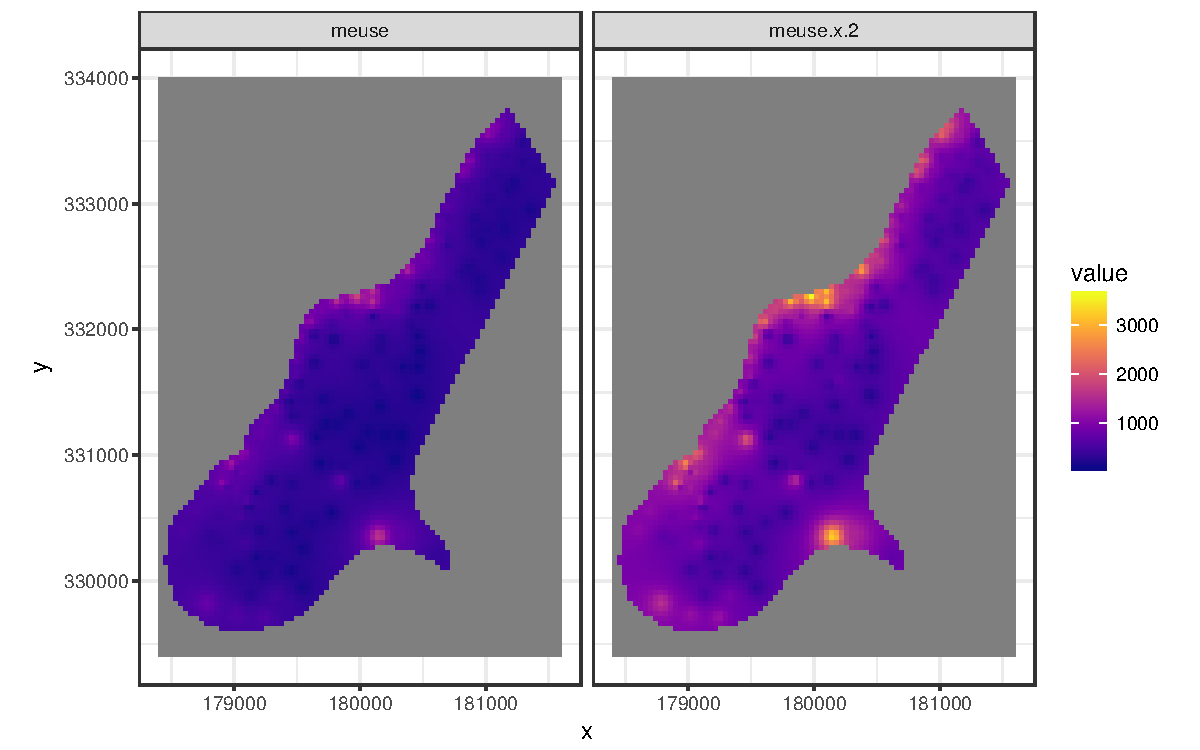
\includegraphics[width=0.8\columnwidth]{spraster2.pdf}
\end{figure}
\end{onlyenv}
\end{overlayarea}
\end{frame}

\subsubsection{绘制地图要素}
\begin{frame}[t,fragile]{\subsecname}{\subsubsecname}
\begin{itemize} 
\item<1-> \emphText{ggsn}包提供\emphText{north}和\emphText{scalebar}函数扩展了ggplot2包指北针和比例尺地图要素的绘制功能
\end{itemize}

\begin{overlayarea}{\textwidth}{\textheight}
\begin{onlyenv}<1>
\begin{figure}[ht]
  \centering 
  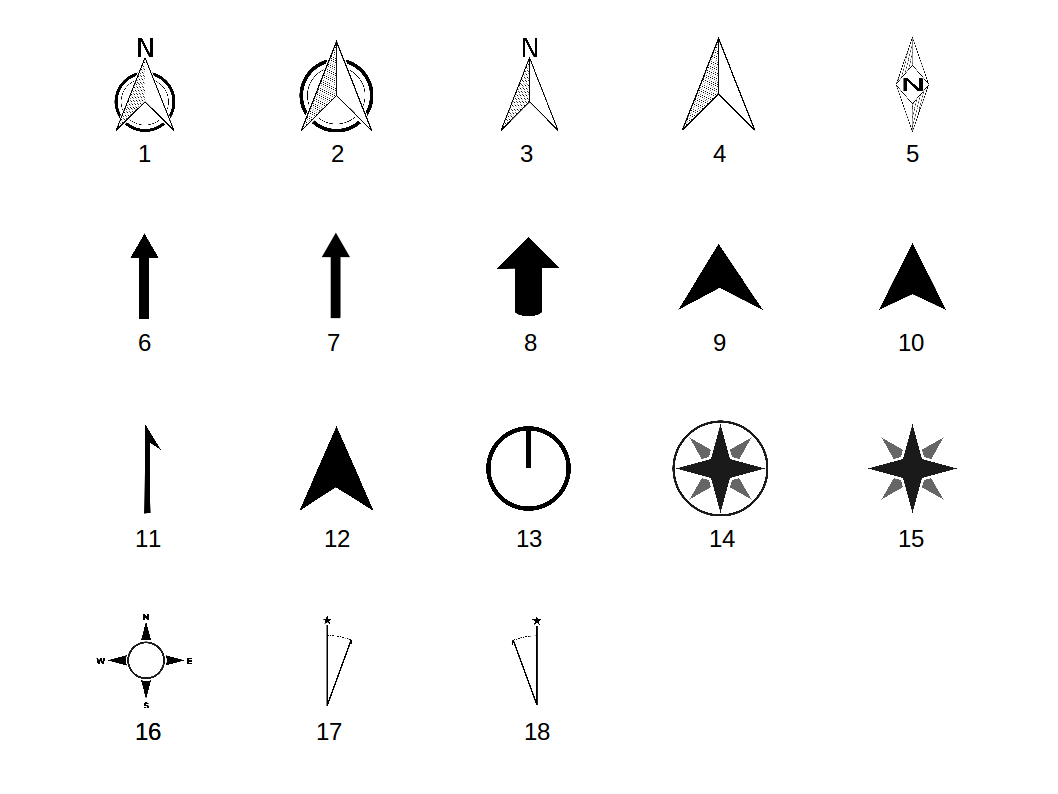
\includegraphics[width=0.75\columnwidth]{northSymbols.png}
  \caption{ggsn提供的指北针样式及编号,原样式来自QGIS}
\end{figure}
\end{onlyenv}

\begin{onlyenv}<2>
\begin{columns} 
\begin{column}{.4\textwidth}
\begin{figure}[ht] 
  \centering 
  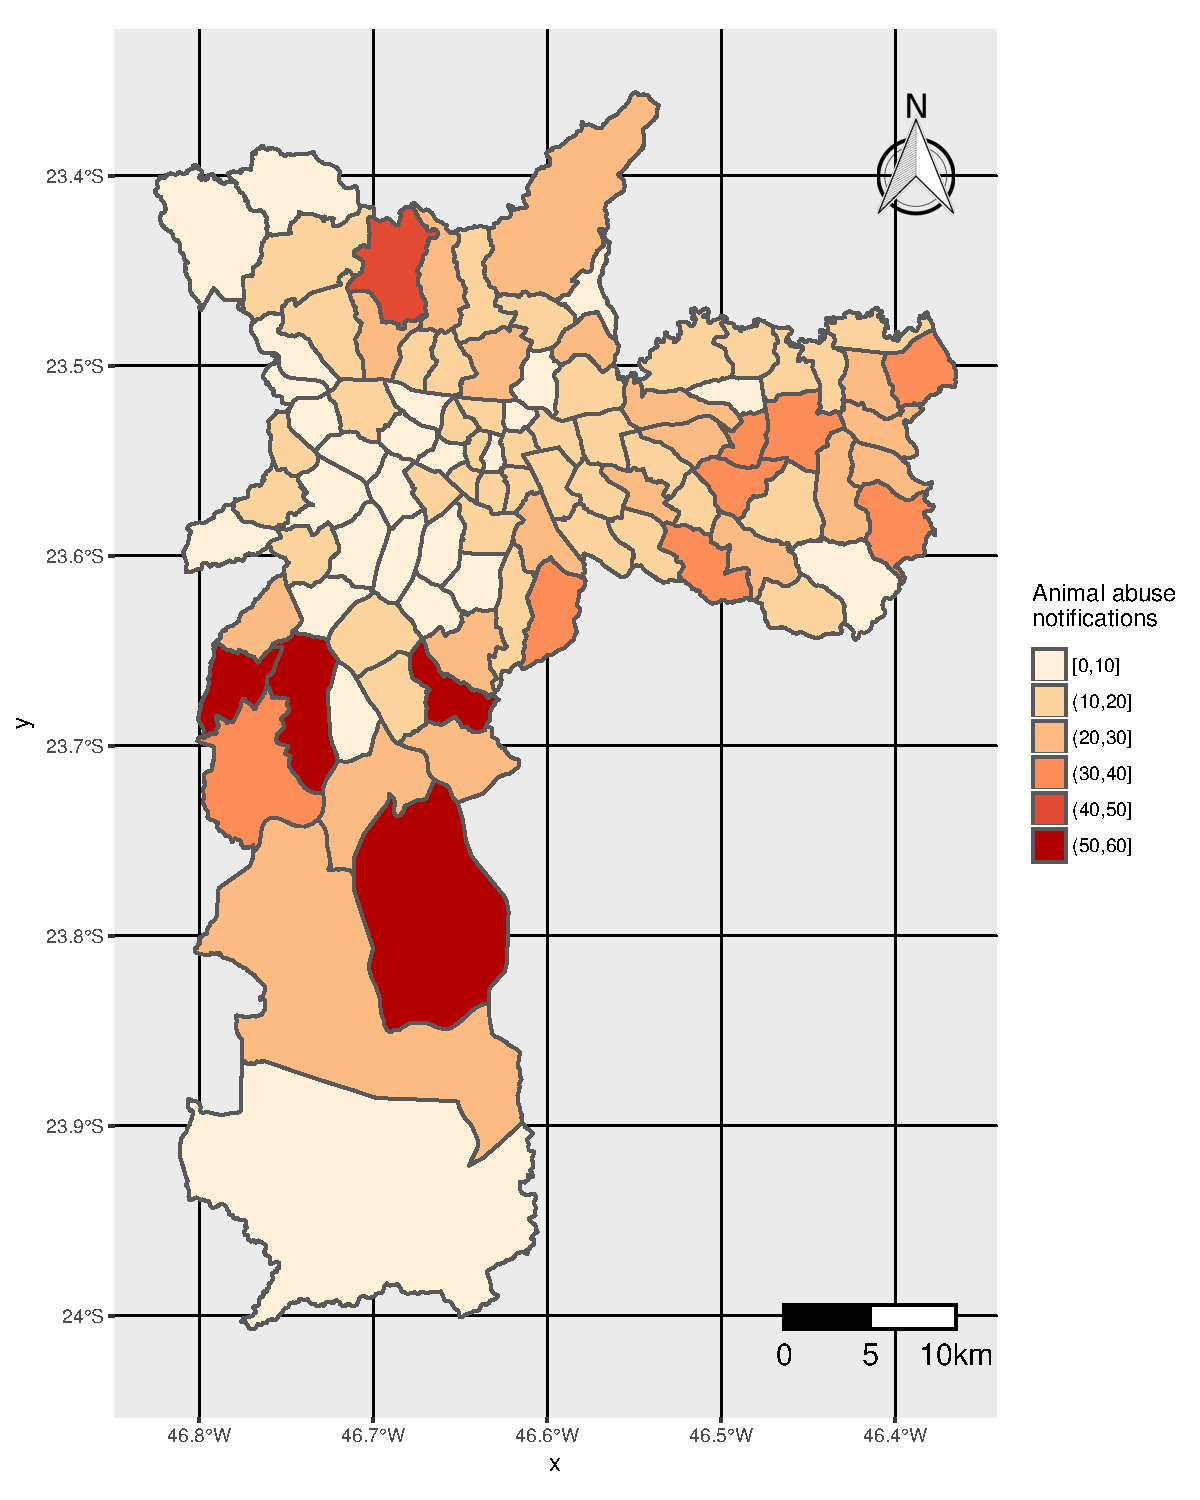
\includegraphics[width=\columnwidth]{ggsn1.pdf}
\end{figure}
\end{column}

\begin{column}{.6\textwidth}
\centering
\begin{rcode}
> library(ggsn);library(sf)
> dsn <- system.file('extdata', package = 'ggsn')
> map <- st_read(dsn, 'sp', quiet = TRUE)
> ggplot(map, aes(fill = nots)) + geom_sf() +
> +    scale_fill_brewer(name = 'Animal abuse\nnotifications', palette = 8) +
> +    |\colorbox{green}{north}|(map) + # 添加指北针
> +     # 在GCS下添加比例尺
> +    |\colorbox{green}{scalebar}|(map, dist = 5, dd2km = TRUE, model = 'WGS84') 
\end{rcode}
\end{column}
\end{columns}
\end{onlyenv}

\begin{onlyenv}<3>
\begin{columns} 
\begin{column}{.4\textwidth}
\begin{figure}[ht] 
  \centering 
  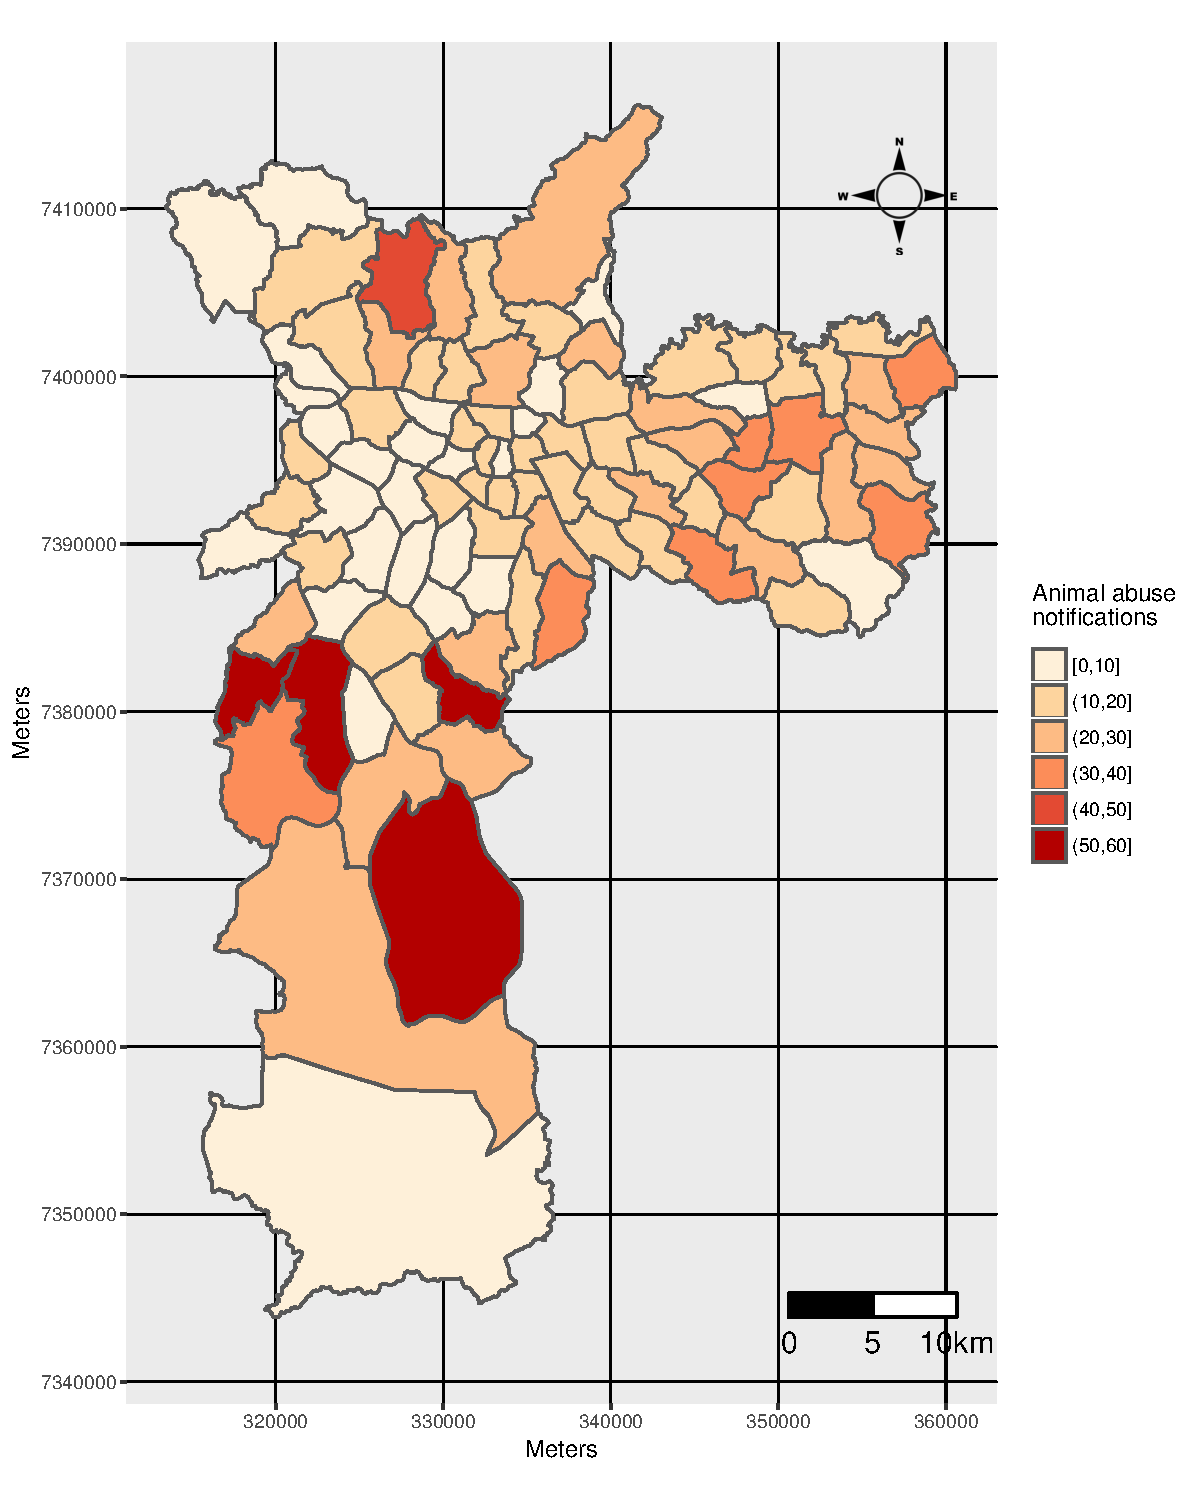
\includegraphics[width=\columnwidth]{ggsn2.pdf}
\end{figure}
\end{column}

\begin{column}{.6\textwidth}
\centering
\begin{rcode}
> # GCS转换到PCS
> map2 <- st_transform(map, 31983)
> ggplot(map2) +
+     geom_sf(aes(fill = nots)) +
+     |\colorbox{green}{north}|(map2, symbol = 16, scale = 0.15) +
+     scale_fill_brewer(name = 'Animal abuse\nnotifications', palette = 8) +
+     |\colorbox{green}{scalebar}|(map2, dist = 5, dd2km=FALSE) +
+     # 坐标轴按照PCS进行转换
+     |\colorbox{green}{coord\_sf}|(datum = st_crs(31983)) + 
+     xlab('Meters') +
+     ylab('Meters')
\end{rcode}
\end{column}
\end{columns}
\end{onlyenv}
\end{overlayarea}
\end{frame}

\subsubsection{叠加瓦片地图图层}
\begin{frame}[t,fragile]{\subsecname}{\subsubsecname}
\begin{itemize} 
\item<1-> \emphText{ggspatial}包是近年来开发比较活跃的一个基于ggplot2的空间数据扩展包,其重写了
所有sp对象的绘图函数,并且还提供叠加OpenStreetMap(OSM)瓦片地图的功能
\end{itemize}

\begin{overlayarea}{\textwidth}{\textheight}
\begin{onlyenv}<2>
\begin{columns} 
\begin{column}{.4\textwidth}
\begin{figure}[ht] 
  \centering 
  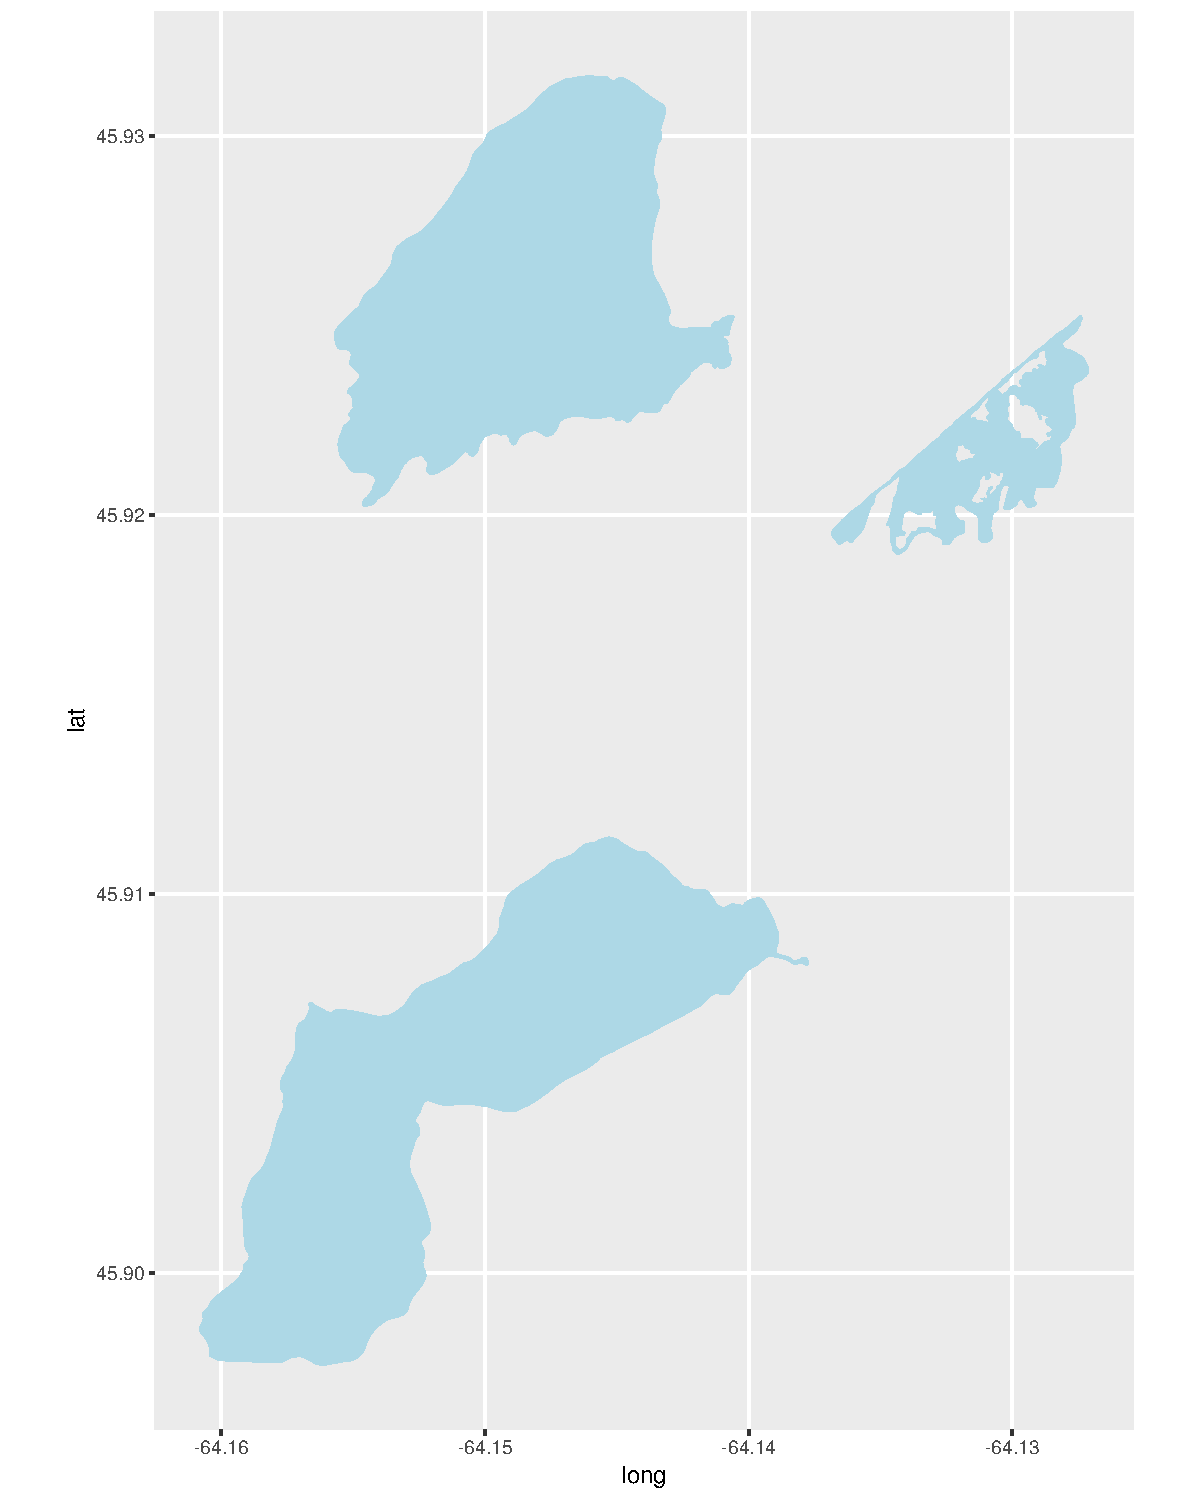
\includegraphics[width=\columnwidth]{ggspatial1.pdf}
\end{figure}
\end{column}

\begin{column}{.6\textwidth}
\centering
\begin{rcode}
> library(ggspatial)
> data(longlake_waterdf)
> class(longlake_waterdf)
[1] "SpatialPolygonsDataFrame"
attr(,"package")
[1] "sp"
# ggspatial函数直接绘制sp对象
# 其是ggplot()+geom\_spatial()+coord\_map()的组合
> |\colorbox{green}{ggspatial}|(longlake_waterdf, fill = "lightblue")
Converting coordinates to lat/lon (epsg:4326)
\end{rcode}
\end{column}
\end{columns}
\end{onlyenv}

\begin{onlyenv}<3>
\begin{columns} 
\begin{column}{.4\textwidth}
\begin{figure}[ht] 
  \centering 
  \includegraphics[width=\columnwidth]{ggspatial2.pdf}
\end{figure}
\end{column}

\begin{column}{.6\textwidth}
\centering
\begin{rcode}
# ggosm根据数据范围自动下载osm瓦片地图
# 其是ggplot()+geom\_osm()+coord\_map()的组合
> |\colorbox{green}{ggosm}|() + 
+     geom_spatial(longlake_waterdf, fill="lightblue")
Converting coordinates to lat/lon (epsg:4326)
Zoom: 15
\end{rcode}
\end{column}
\end{columns}
\end{onlyenv}
\end{overlayarea}
\end{frame}

\begin{frame}[t,fragile]{\subsecname}{\subsubsecname}
\begin{itemize} 
\item<1-> \emphText{ggmap}是另一个常用的在ggplot2中叠加瓦片地图图层的包;而且除了osm之外,还可以
加载Google Maps和Stamen Maps
\end{itemize}

\begin{overlayarea}{\textwidth}{\textheight}
\begin{onlyenv}<2>
\begin{columns} 
\begin{column}{.4\textwidth}
\begin{figure}[ht] 
  \centering 
  \includegraphics[width=\columnwidth]{ggmap.pdf}
\end{figure}
\end{column}

\begin{column}{.6\textwidth}
\centering
\begin{rcode}
> library(ggmap)
> sp <- |\colorbox{green}{get\_googlemap}|("圣保罗")
> bb <- c(st_bbox(map) * matrix(rep(c(1.001, 0.999), e = 2), ncol = 2))
> nms <- names(attr(sp, "bb"))
# 给瓦片地图设置bbox
> attr(sp, "bb")[1, ] <- bb[c(2, 1, 4, 3)]
# ggmap和geom\_sf不兼容,这里采用sp对象转换的方案
> map_sp <- readOGR(dsn, "sp")
> map_sp@data$id <- 0:(nrow(map_sp@data) - 1)
> map_sp <- merge(tidy(map_sp), map_sp, by = 'id') 
# 如果要将ggmap获取的瓦片地图和sf包兼容,
# 可以使用sf包重写的plot函数,
# 其提供bgMap参数将ggmap对象作为底图叠加
> |\colorbox{green}{ggmap}|(sp) +
>     geom_polygon(data = map_sp, aes(long, lat, group = group, fill = nots), alpha = .7) +
>     coord_equal() + blank() +
>     geom_path(data = map_sp, aes(long, lat, group = group)) +     
>     scalebar(map_sp, dist = 5, dd2km = T, model = 'WGS84') +
>     north(map) +
>     scale_fill_brewer(name = 'Animal abuse\nnotifications', palette = 8) +
>     theme(legend.position = c(0.9, 0.35))
\end{rcode}
\end{column}
\end{columns}
\end{onlyenv}
\end{overlayarea}
\end{frame}
%而栅格空间数据可以直接用ggplot2包的\emphText{geom\_raster}或\emphText{geom\_tile}函数来绘制
%\item<2-> 基于ggplot2包绘制地图要素可以借助\emphText{ggsn}包